% !TEX root = ../thesis.tex
\chapter{Web App Pages}
\label{app:web_designs}

\begin{figure}[h]
	\centering
	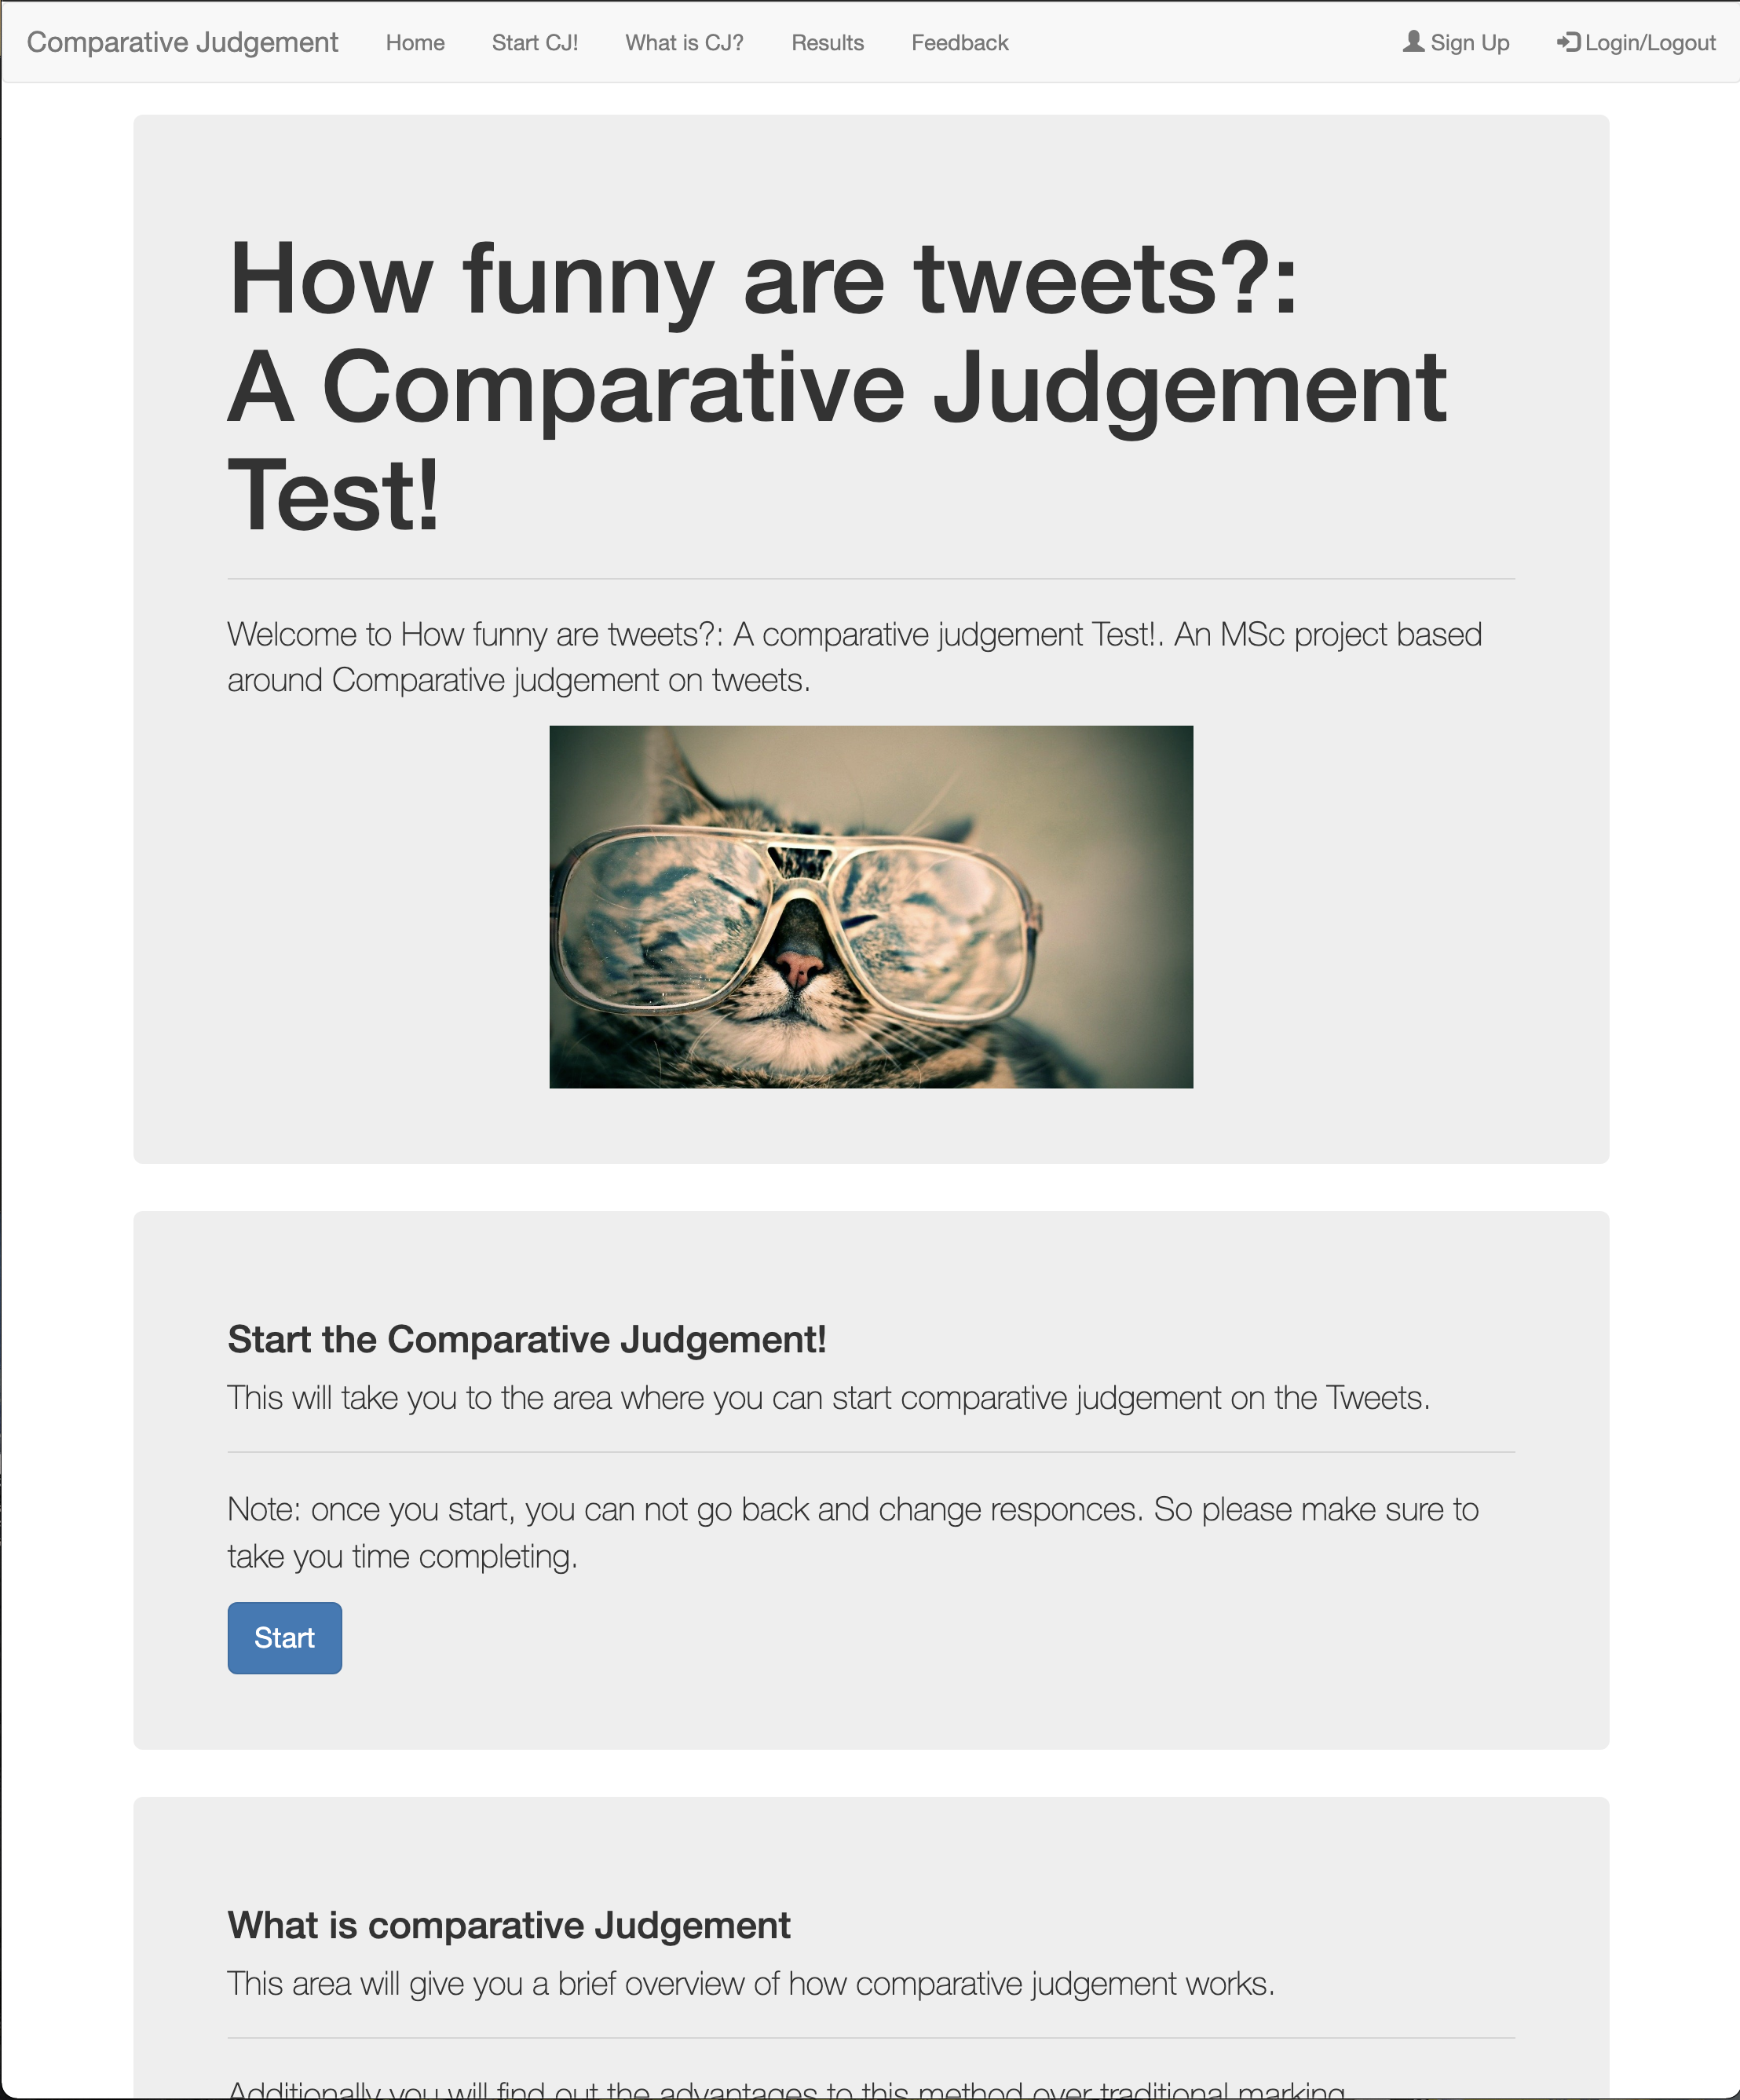
\includegraphics[width=\textwidth]{Home_page.png}
	\caption{}
	
		
	\end{figure} 
\begin{figure}[h]
	\centering
	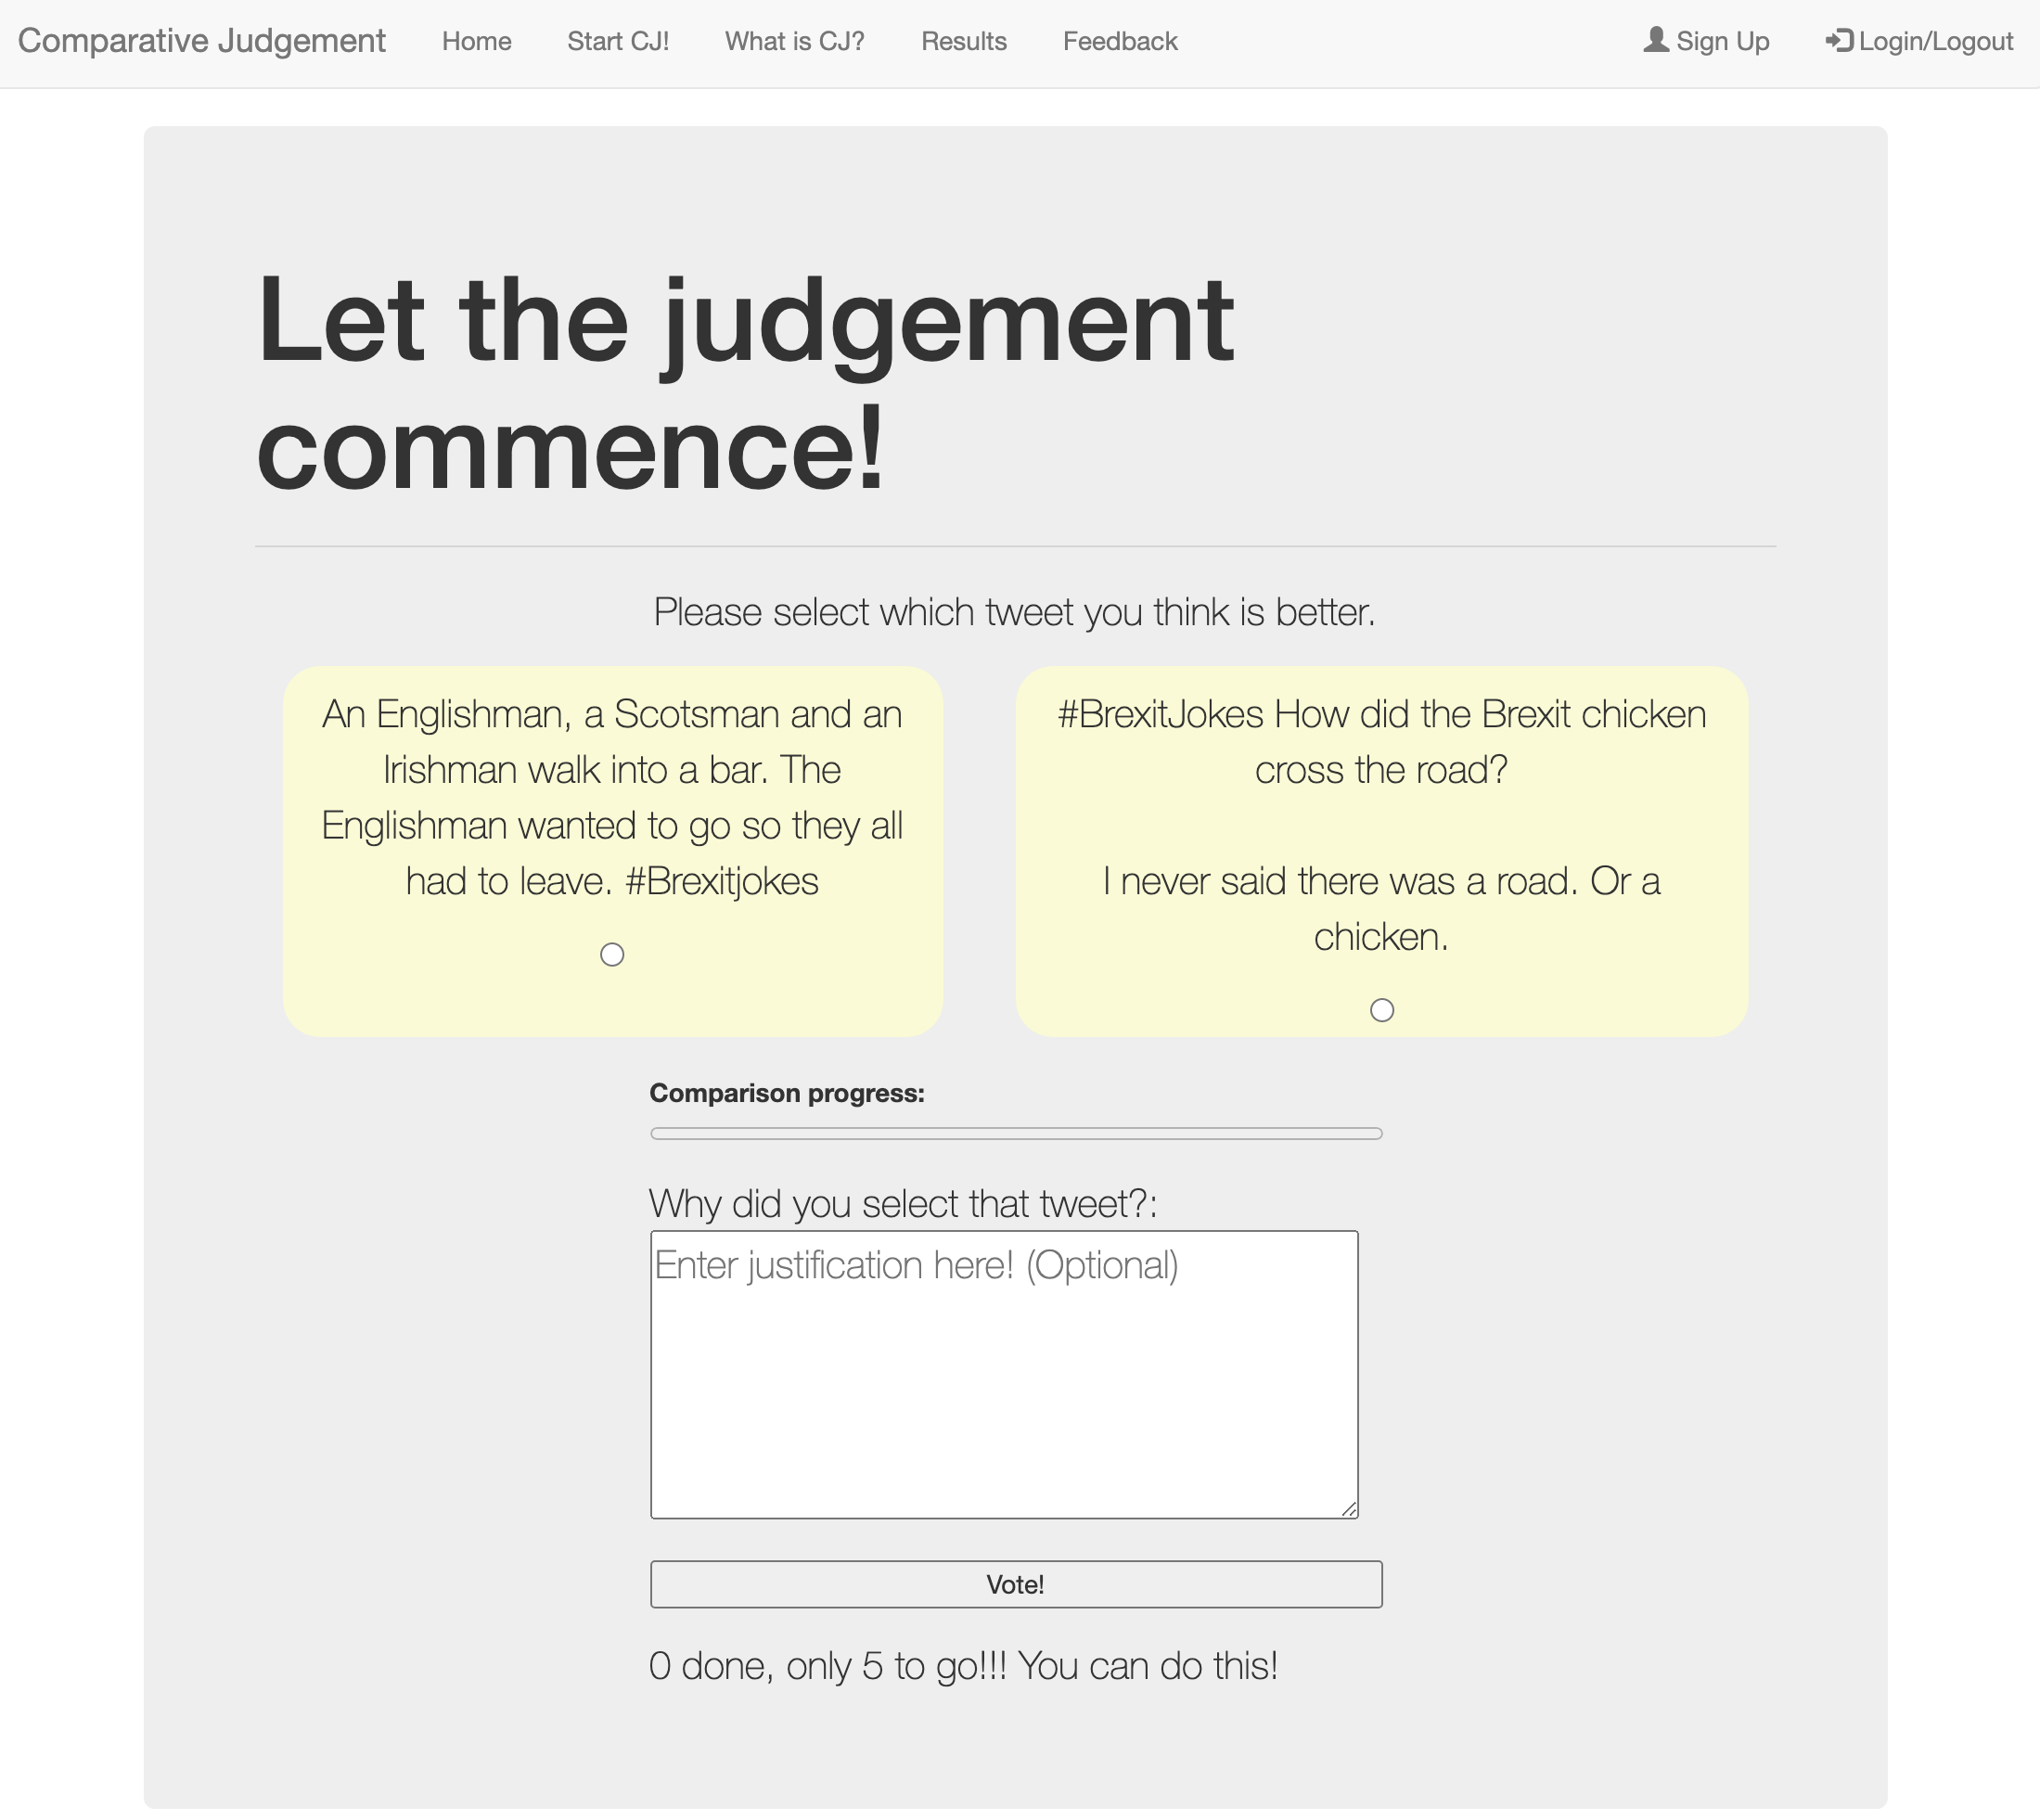
\includegraphics[width=\textwidth]{Compare.png}
	\caption{}
	
		
	\end{figure} 

\begin{figure}[h]
	\centering
	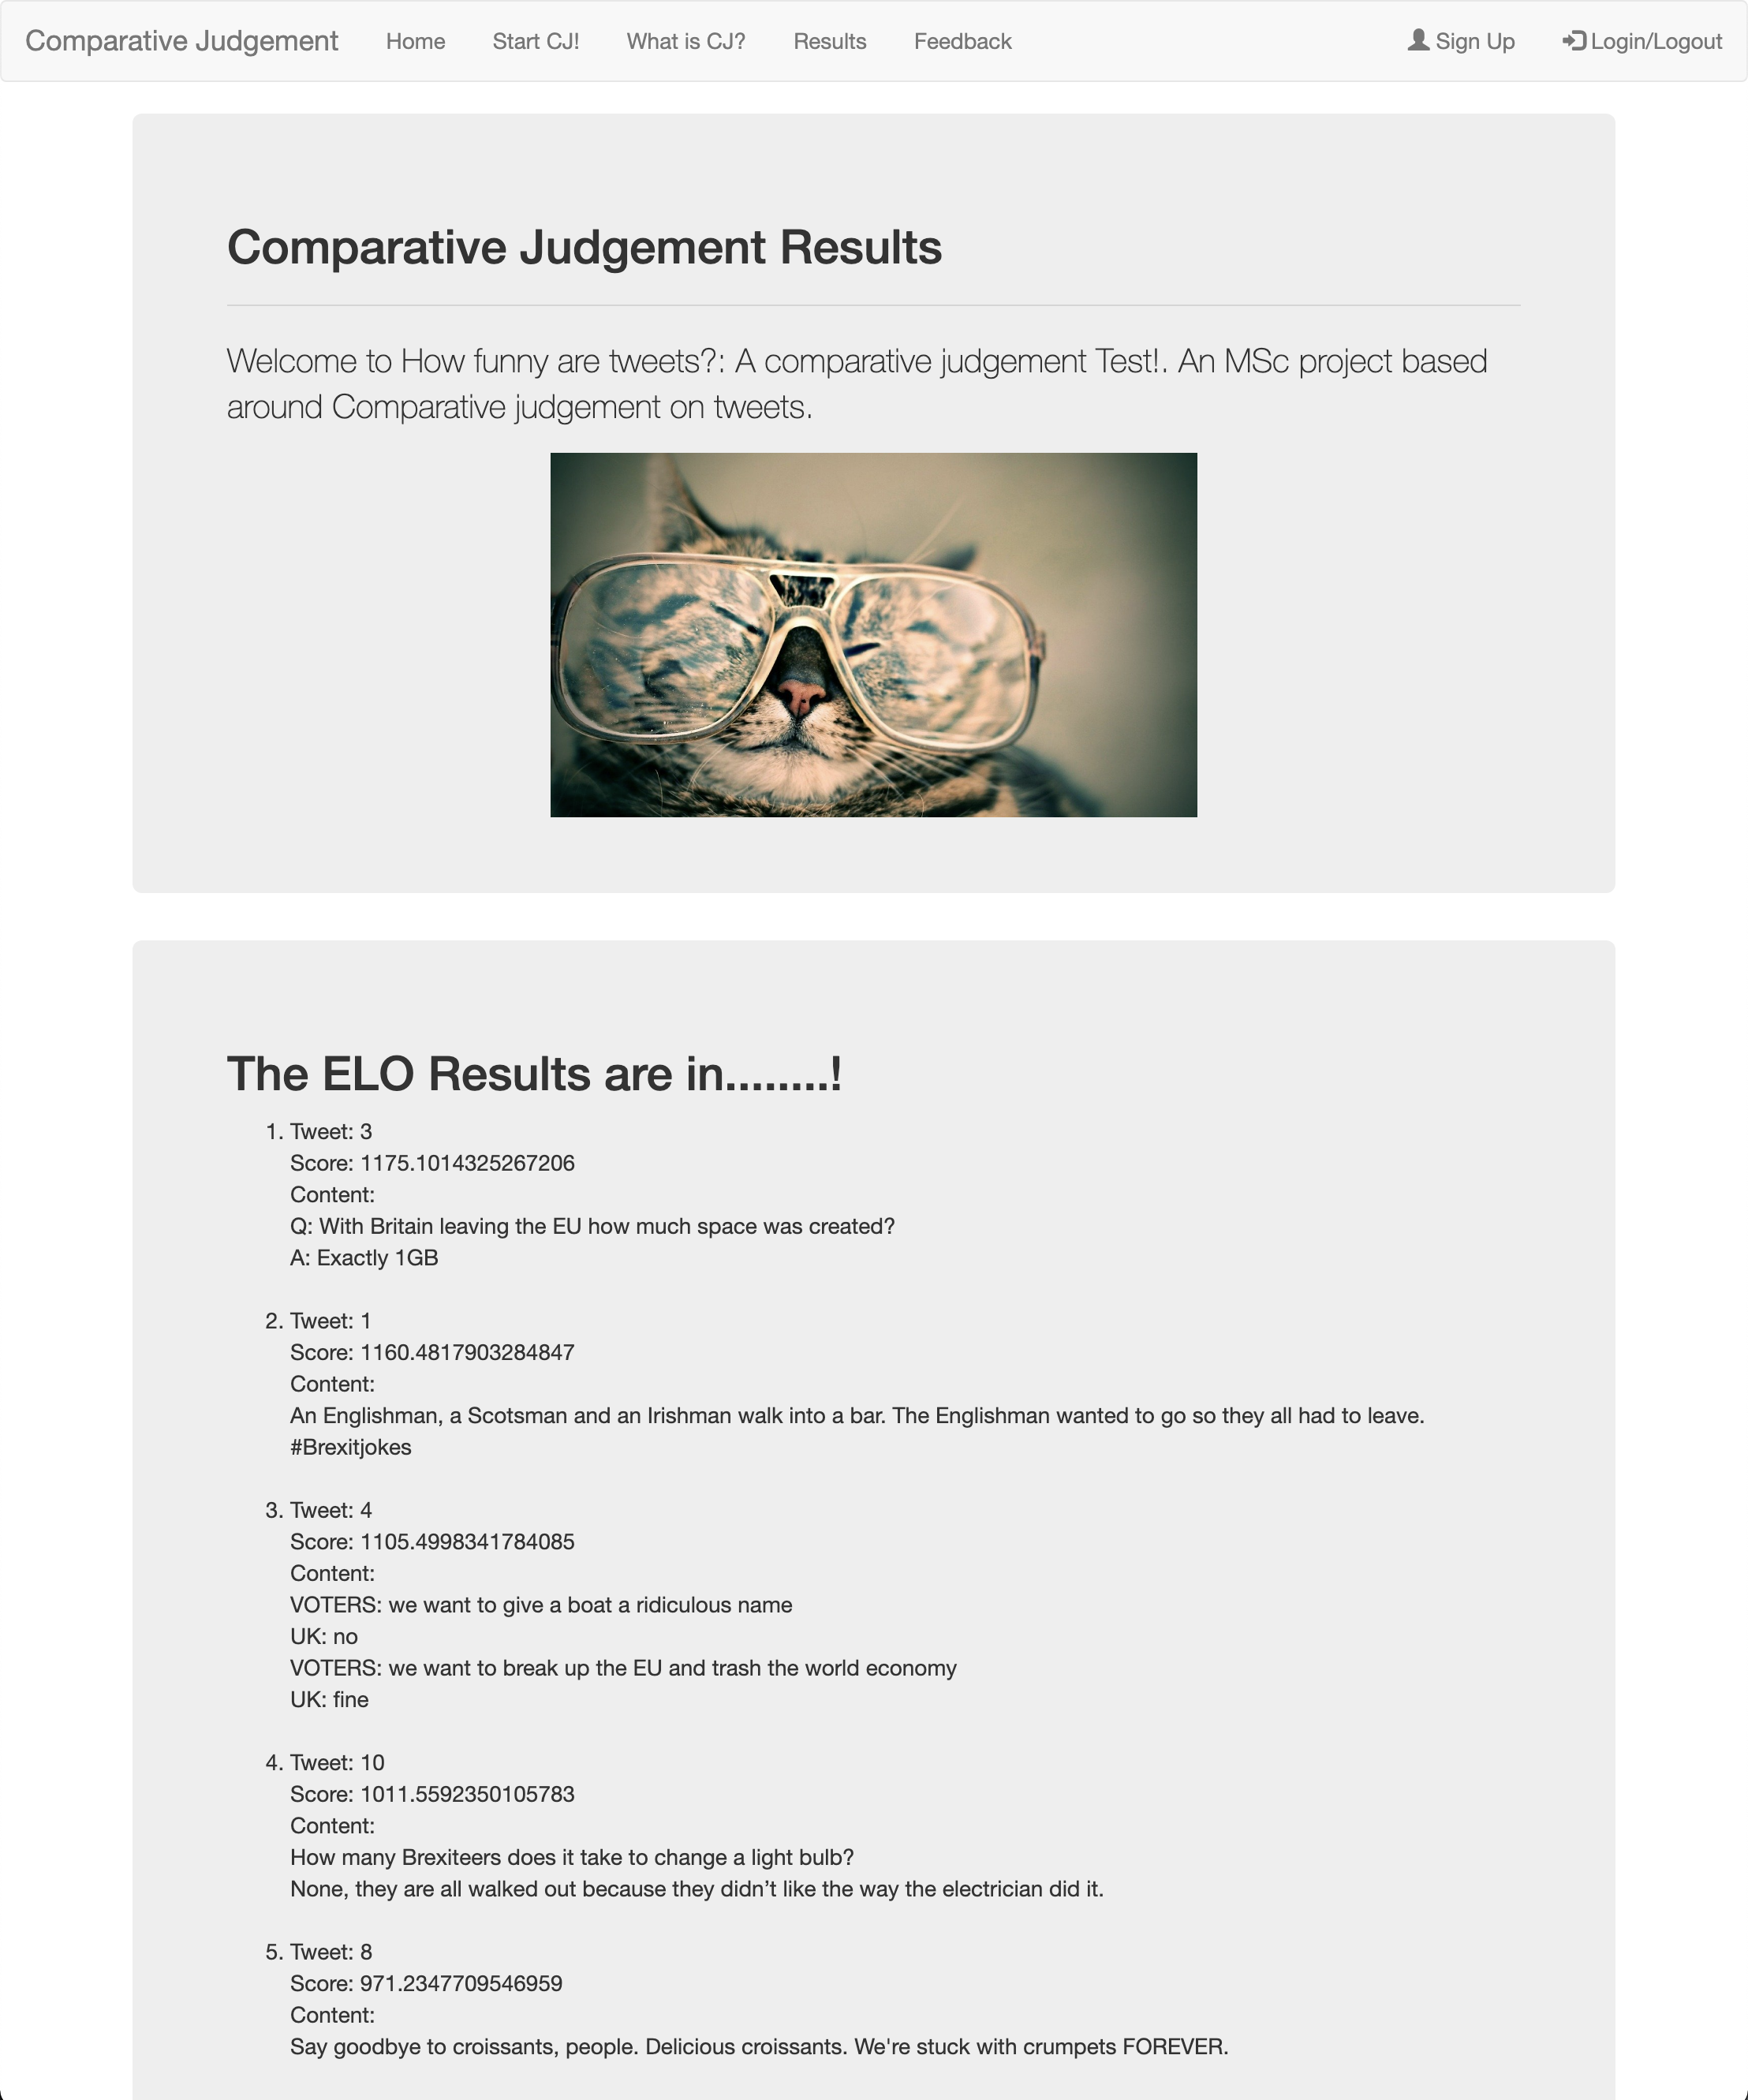
\includegraphics[width=\textwidth]{Results.png}
	\caption{}
	
		
	\end{figure} 

%\begin{figure}[h]
%	\centering
%	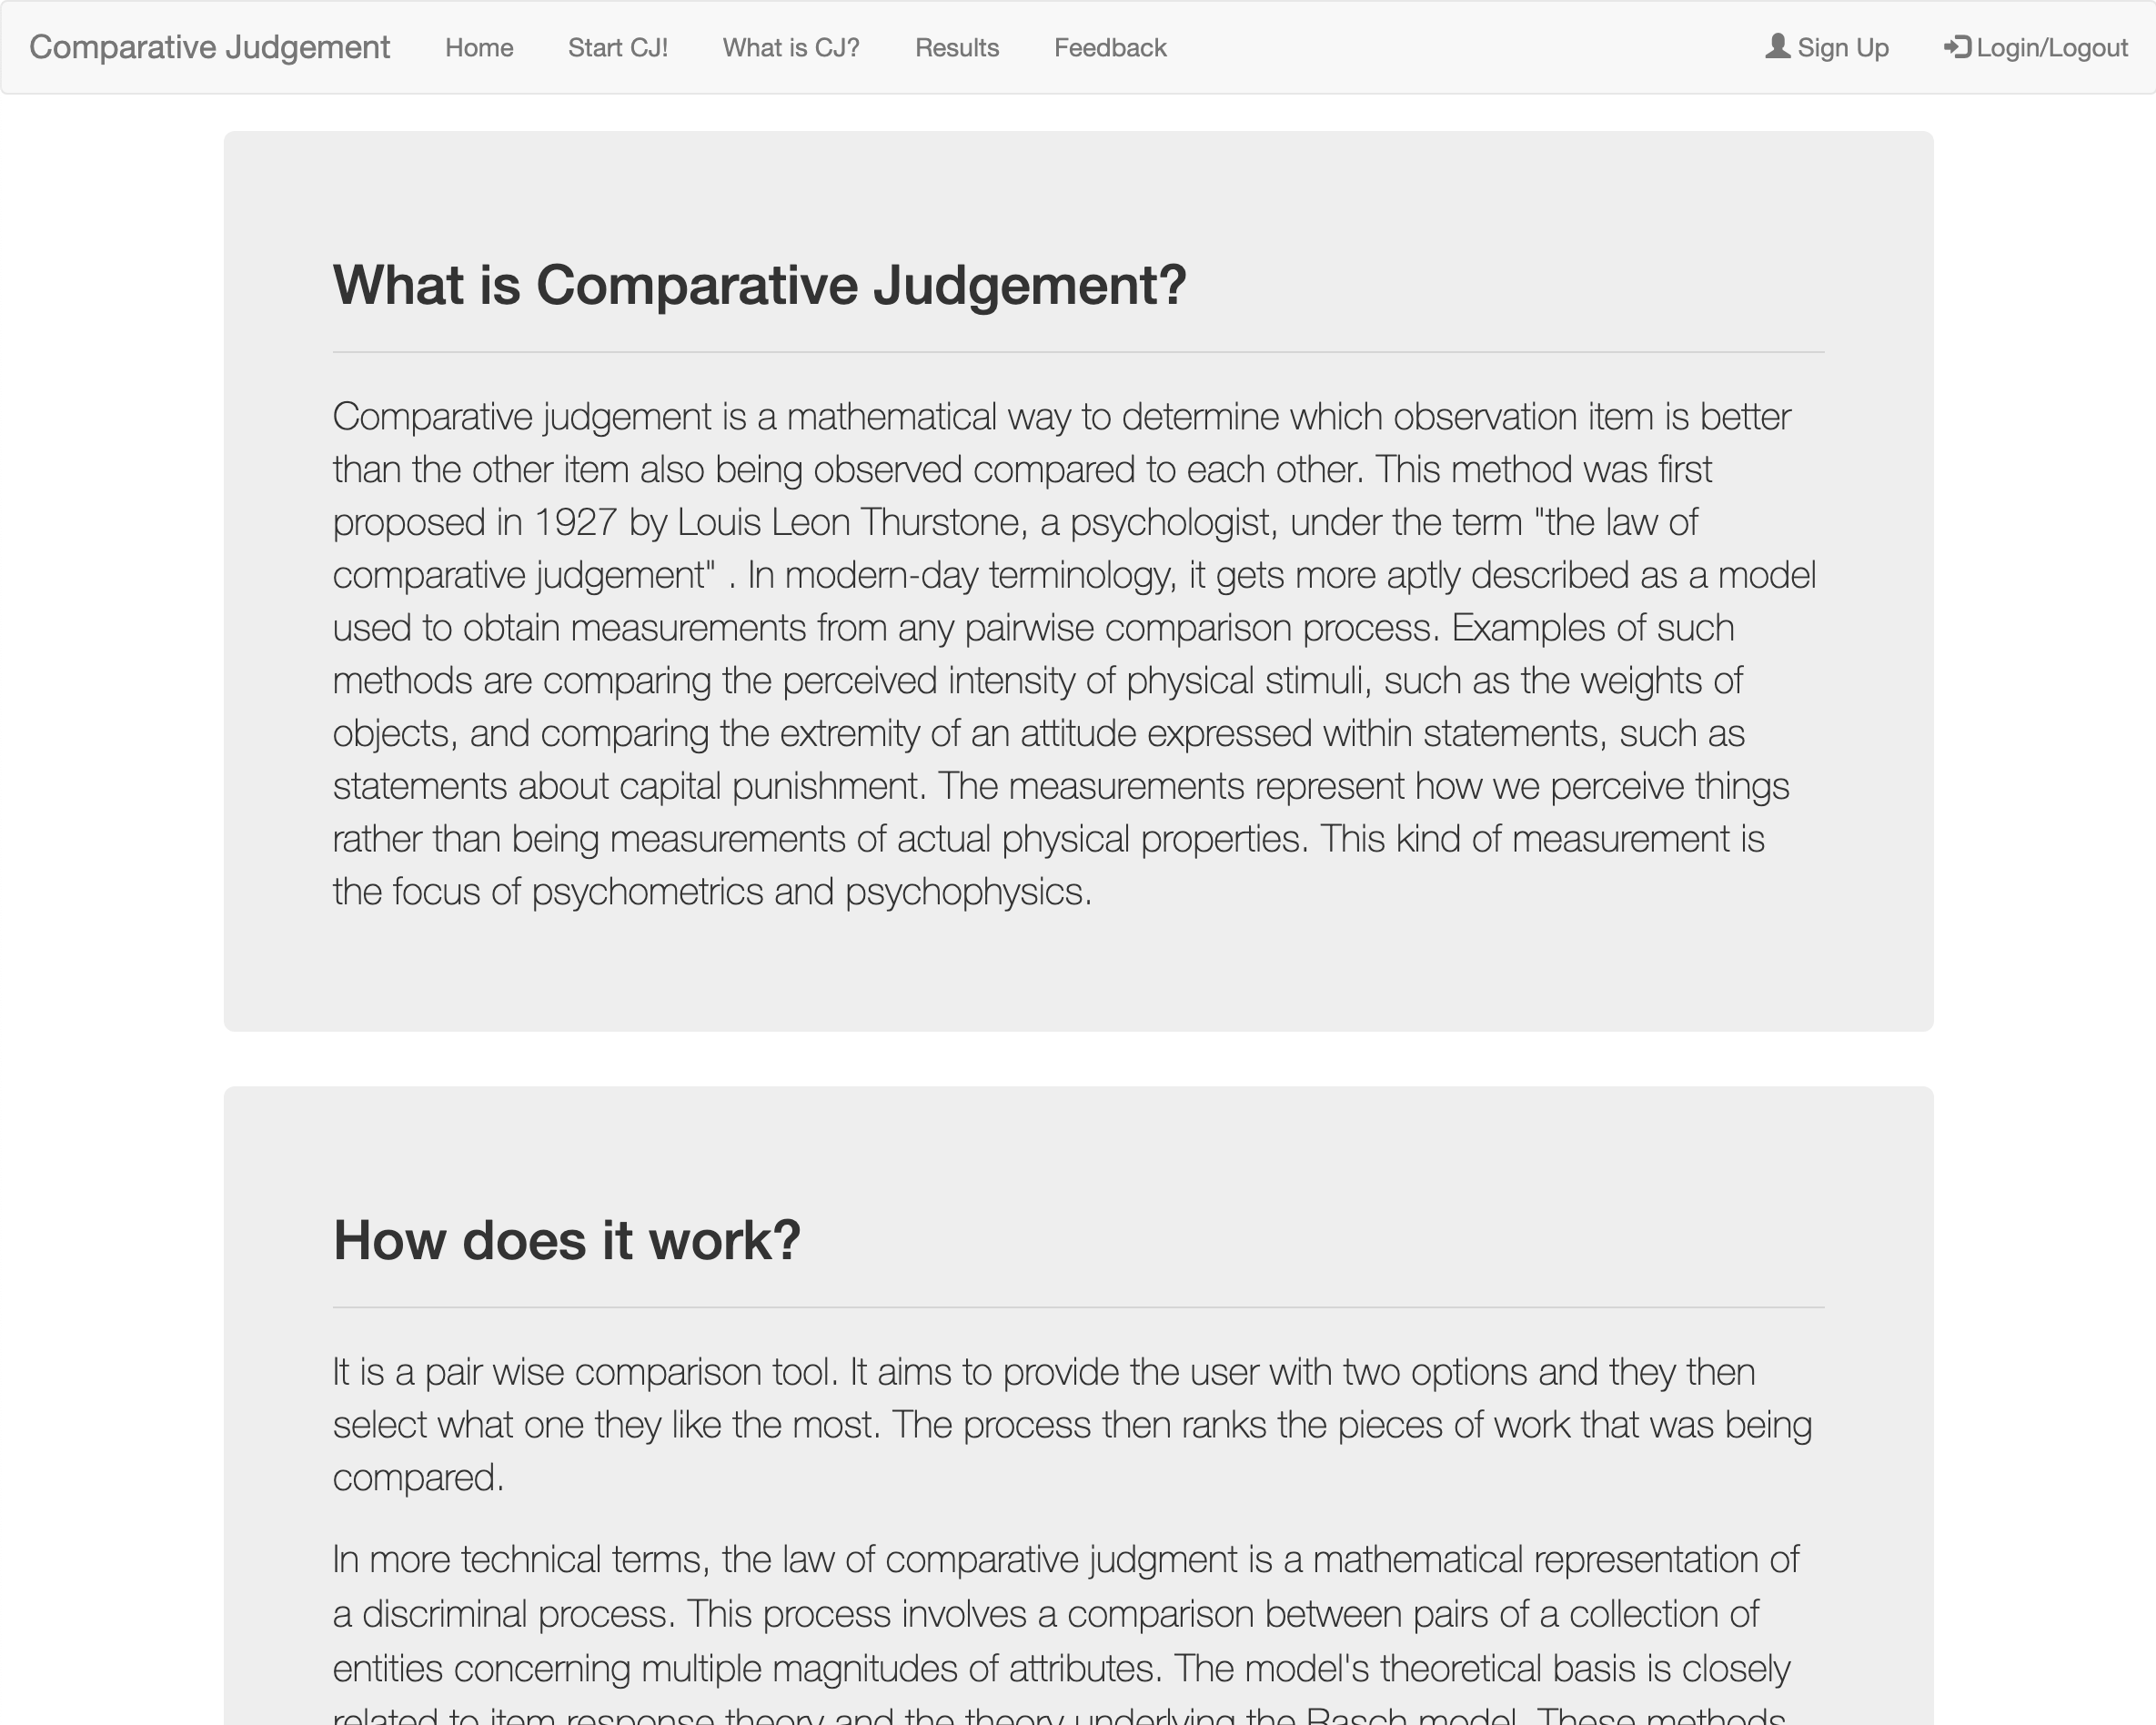
\includegraphics[width=10cm]{What_is_CJ.png.png}
%	\caption{}

		
%	\end{figure} 
\begin{figure}[h]
	\centering
	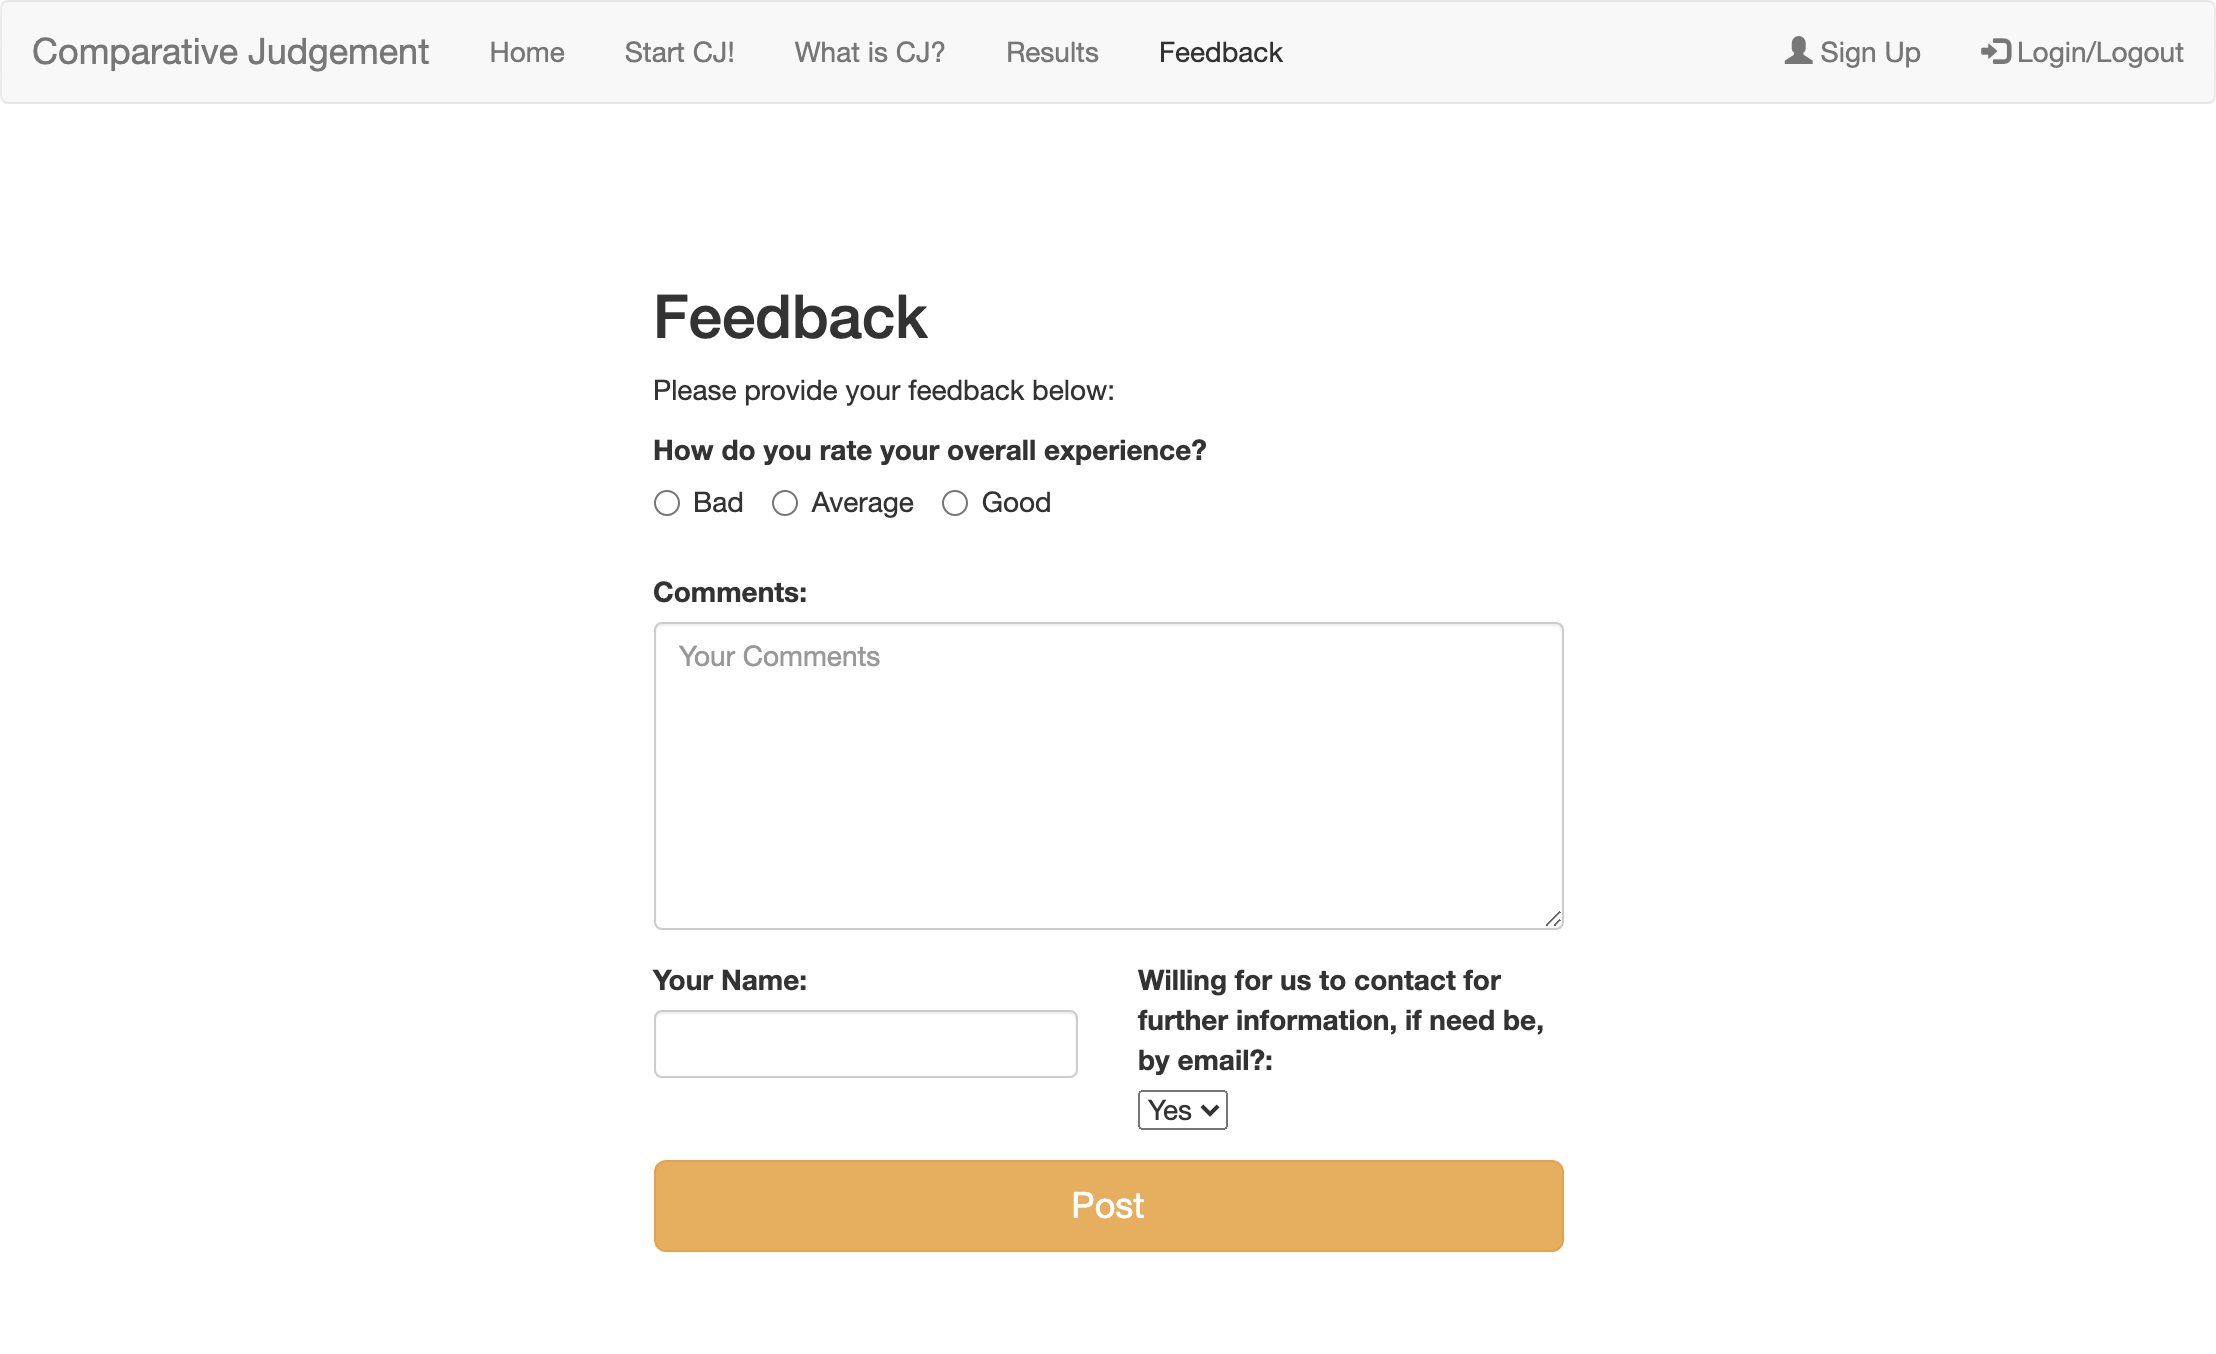
\includegraphics[width=\textwidth]{feedback.png}
	\caption{}
		
	\end{figure} 

%\begin{figure}[h]
%	\centering
%	\includegraphics[width=10cm]{login.png}
%	\caption{}
	
%\end{figure} 


%\begin{figure}[h]
%	\centering
%	\includegraphics[width=10cm]{signup.png}
%	\caption{}
	
%\end{figure} 

\chapter{Designs}
We will next look at the initial designs compared against the file outcome of the web app. We will also explain the decisions made and what changes we made, and why. 

In total, there are five different pages within the web app. The web app has a home page, facilitates the comparative judgment procedure, results, and feedback.

\subsection{Home Page}

\subsection{Comparison Page}

\subsection{What is Comparative Judgement Page}

\subsection{Results Page}

\subsection{Feedback Page}


\chapter{Risks}


\begin{center}
	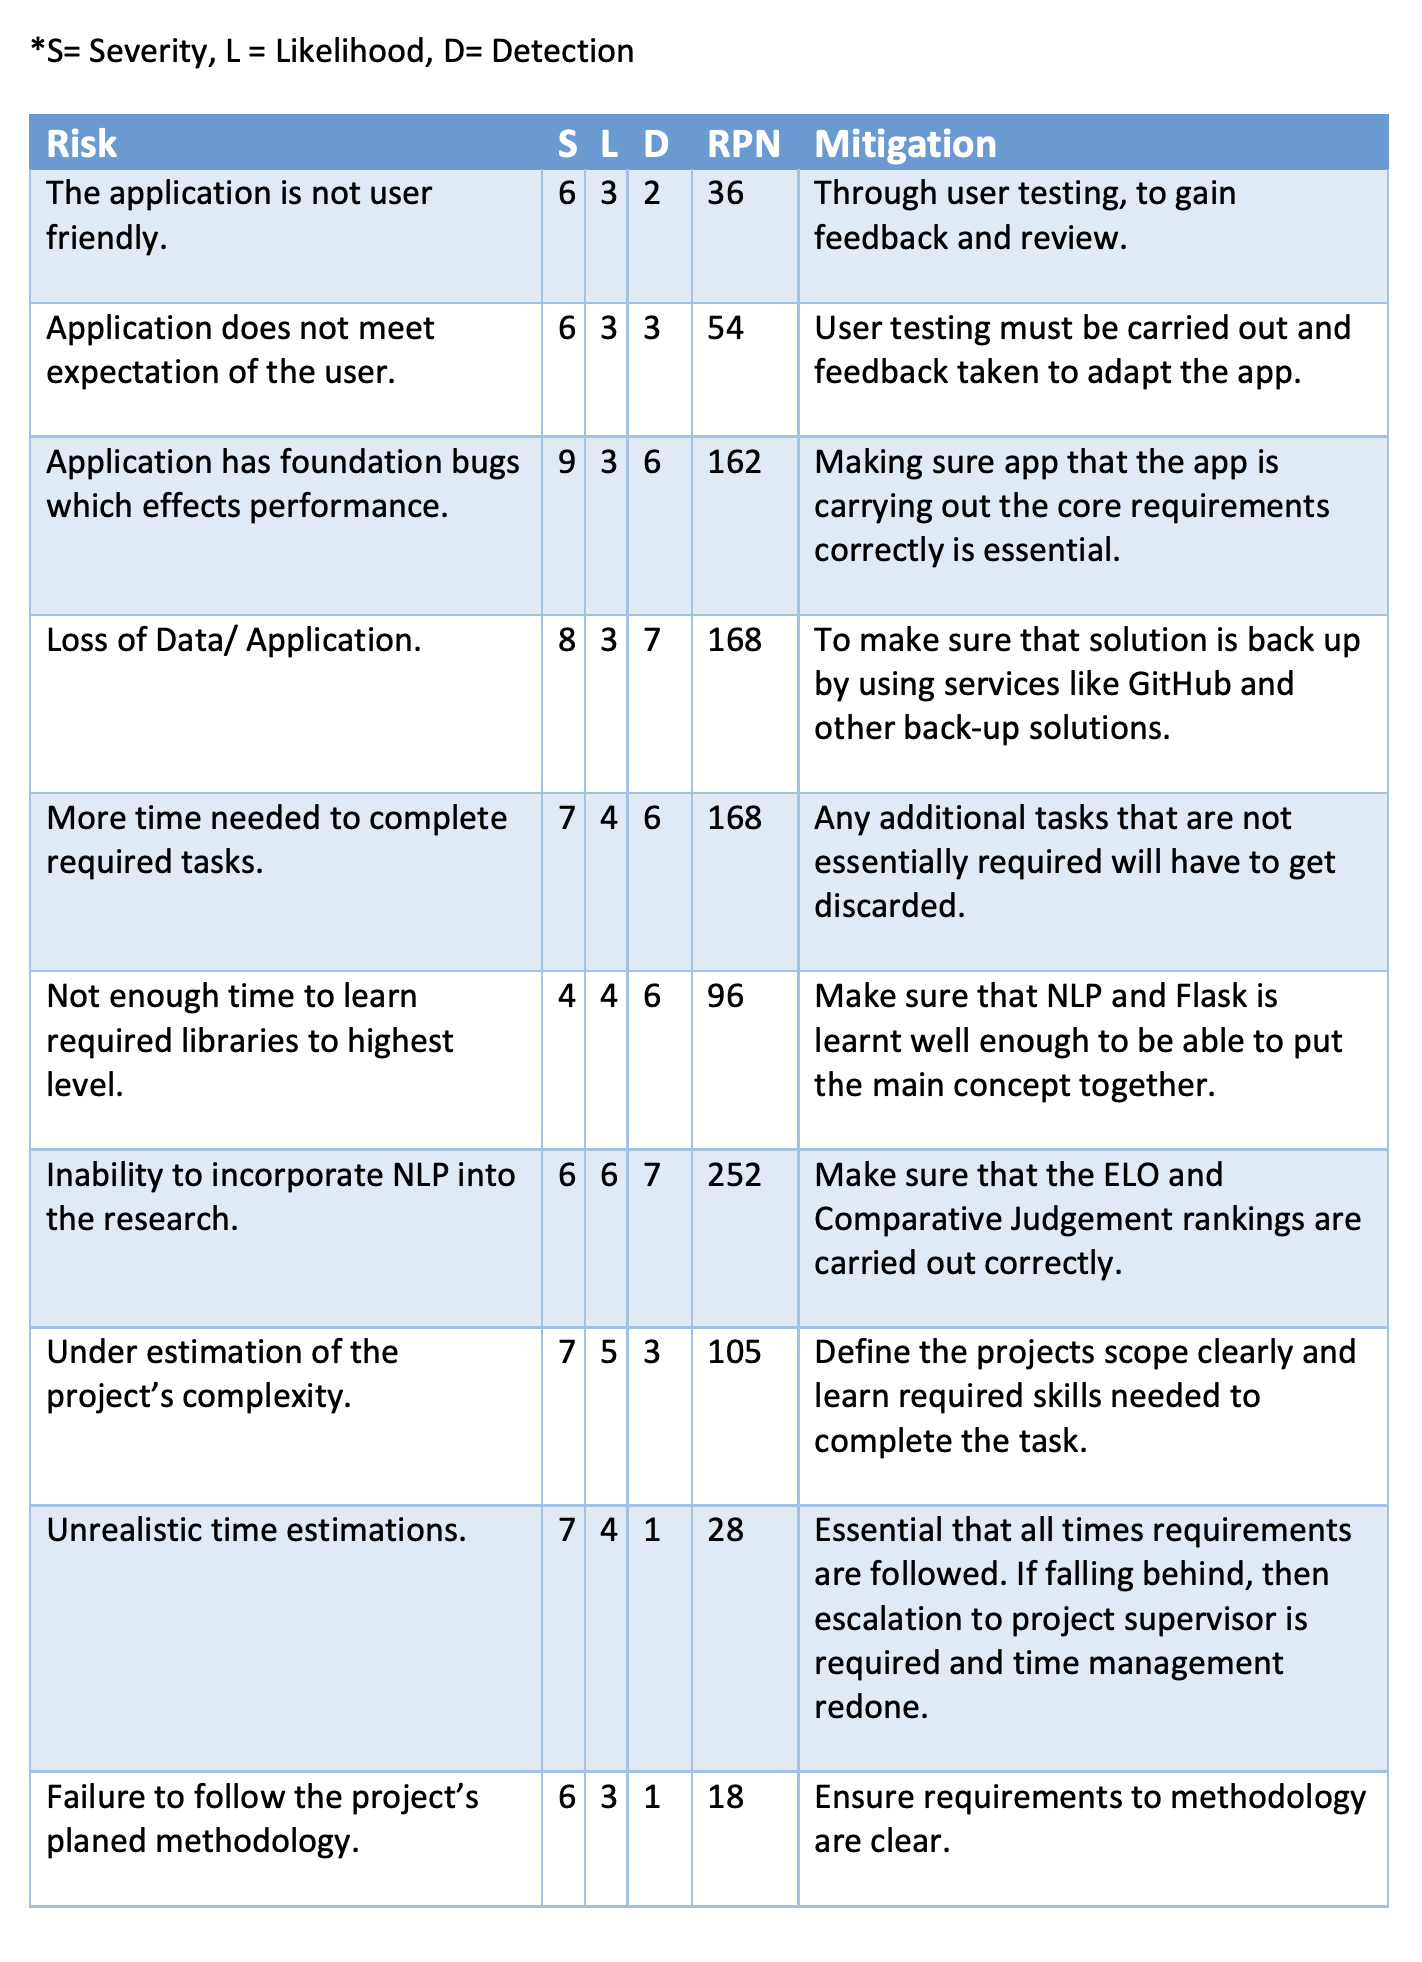
\includegraphics[width=11.5cm]{risk_table.png}
	%\caption{A visual representation of the processes pipline.}...
\end{center}




\begin{landscape}
	\chapter{Schedule}
		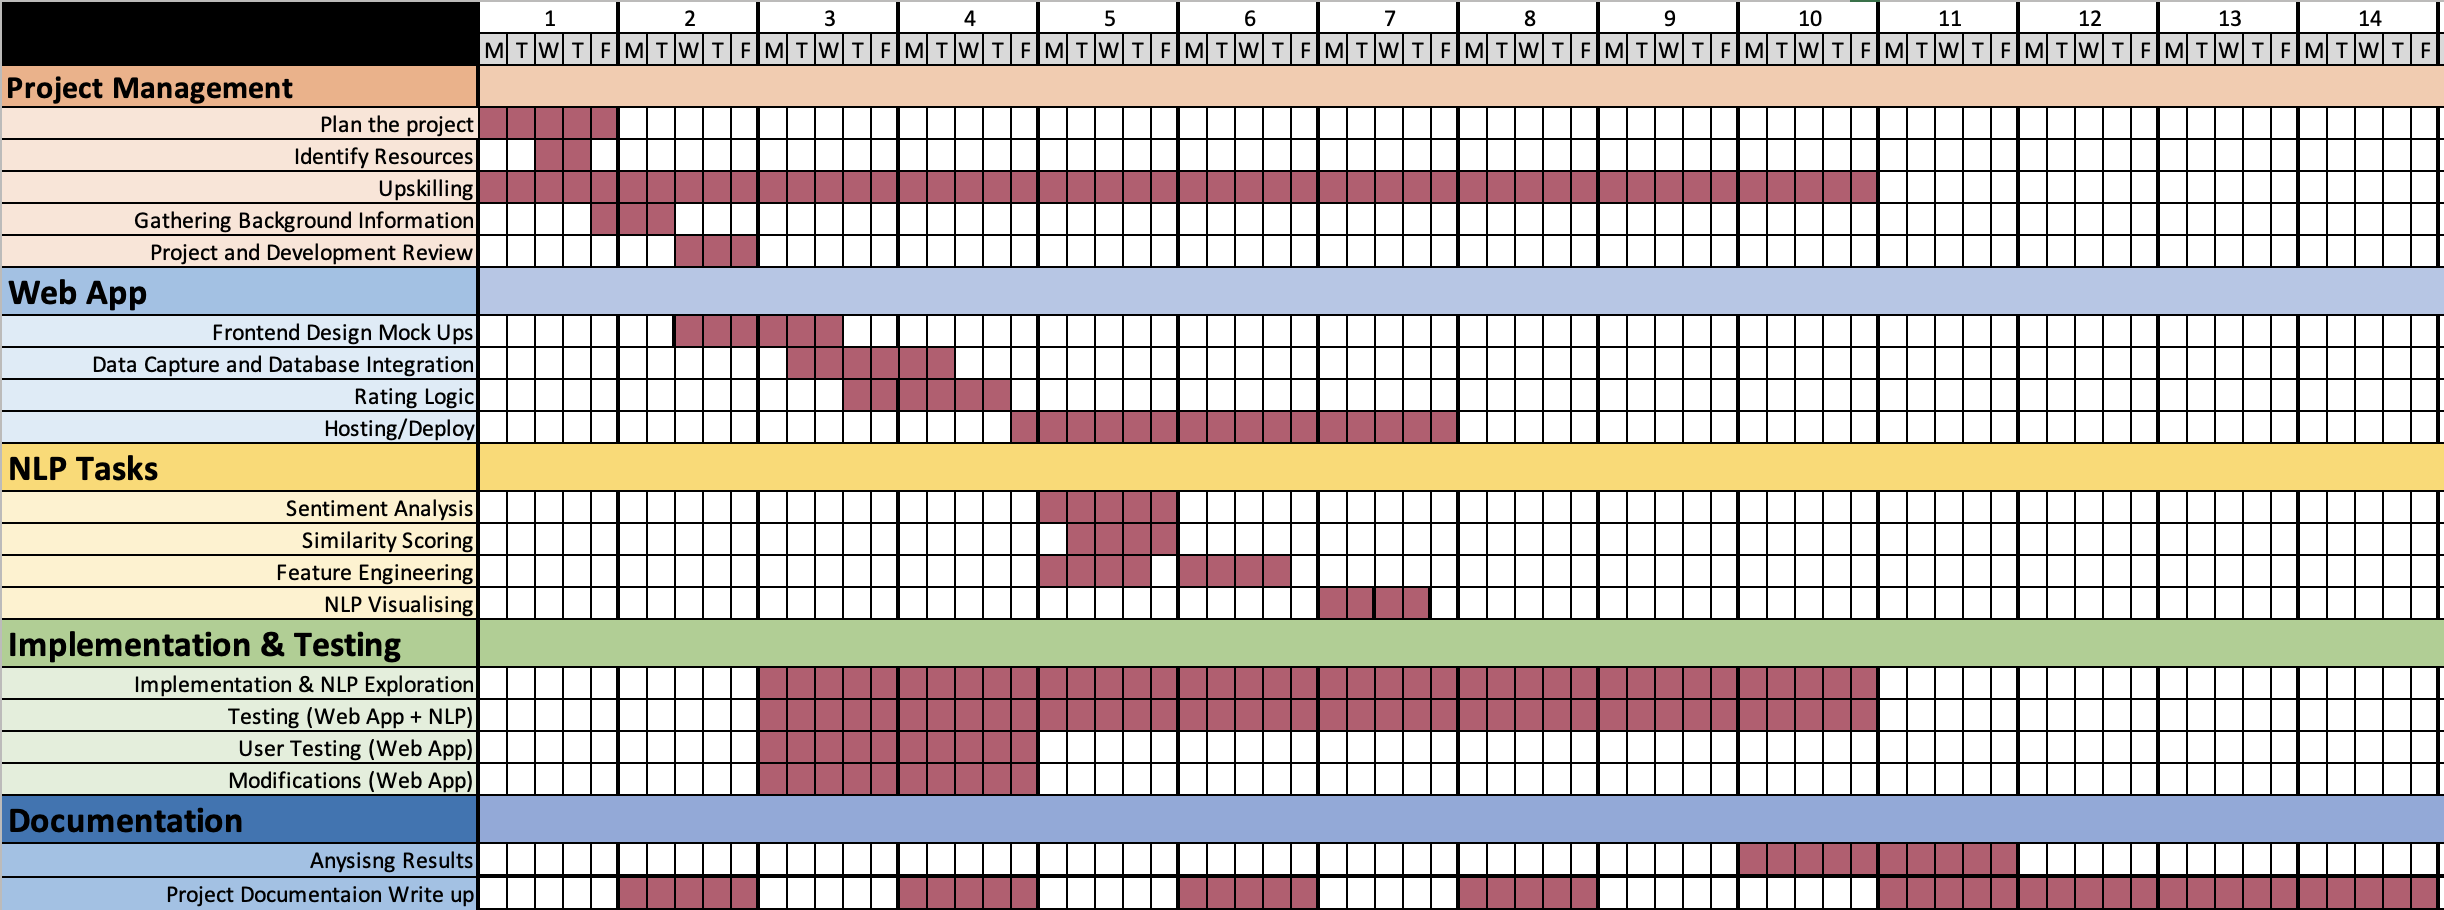
\includegraphics[width=21cm]{ganttchart.png}
\end{landscape}

\chapter{Software Development Life Cycle Methodology}
Project management is crucial for any task that is about to be carried out, even more so for software development. As a famous Benjamin Franklin quote says, "Failing to plan is planning to fail" \cite{plan_to_fail}. With this in mind, we must decide on the suitable project planning method that compliments our initial software design. From the waterfall method to Rapid application development (RAD) or the more modern methods of agile development, there are many methods that we could choose. We will explain the different methods we could use and what would be best for our solution and intended development method.

The profession of the software developer has existed since the first computers, but the practices and methods for developing software have evolved over timer \cite{SDLC}. The approaches have developed over the years to adapt to the ever-changing landscape of software development. The methods, known as software development life cycles (SDLC), vary in approach but fundamentally share the same goal. The main aims of the SDLC are to break the development up into stages. However, what changes with different SDLC is how these stages get carried out. The different stages are planning, requirements, designing and prototyping, software development, testing, deployment, operations, and maintenance \cite{SDLC}.

The first stage, planning, involves resource allocation, capacity planning, project scheduling, cost estimation, and provisioning \cite{SDLC}. The primary outcome of this stage is to have an overall plan of what we have and what we will need to complete our goal within the constraints like costs and times allowed. The second stage, requirements, is where Subject Matter Experts (SMEs.) guide on what would be needed to carry out the stakeholders' requirements \cite{SDLC}. The third stage, design and prototyping, is where the software architects and developers begin to design the software. The outcome of this stage would be documentation on the intended design patterns and design wireframes of the intended final software. The fourth stage, development, is where the software starts to get made based on the decisions made in design and prototyping, following the chosen methodology. The outcome will be testable, tangible software. The fifth stage, testing, is considered the most crucial stage \cite{SDLC}. It is essential to do all the code quality checking, unit testing, integration testing, performance testing and security testing. The sixth but by no means the final stage is deployment. This stage is when the code is ready to be shipped to the client or uploaded to the required app stores. However, the final stage is operations and maintenance. This stage is about ensuring that the software is getting used as it should and that any bugs that did not initially get picked up in testing are correct and removed from the software. 

%\subsubsection{Waterfall Method}
The waterfall method is a model where each section needs to be completed before moving onto the next stage, like a waterfall flowing down. For example, before we can start analysing the requirements, we need to complete the planning stage. Following the seven critical stages of SDLC, one after the other.

Like all models, they have their advantages and disadvantages. Advantages that this model has is that it is easy to use and follow, and by the way it is all set up, every stage will get finished before the next stage starts. The waterfall method also allows for the project to be easily managed, resulting in easier documentation \cite{cscm01slidesl5}. However, some of the disadvantages are that it is not very useful if the requirements are not very clear at the beginning. Another disadvantage is that once we have moved to the next stage, it is tough to go back to a previous stage to make any changes which therefore creates higher risks to development and has less flexibility \cite{cscm01slidesl5}. The model is best when changes in the project are stable, and the project is small, with the project requirements are clearly defined.

%\subsubsection{RAD: Rapid Application Development}
The overall aim of RAD is to create software projects with higher quality and faster by gathering requirements through workshops or focus groups. Then prototyping the product and then using reiterative user testing of designs early. RAD is the best model for when we need something created quickly and have a pool of users available to test prototypes. However, this approach can be costlym \cite{cscm01slides}. 

%\subsubsection{Spiral Method}
The Spiral Model is an SDLC methodology that aids in choosing the optimal process model. It combines aspects of the incremental build model, waterfall model and prototyping model but is different by a set of six invariant characteristics \cite{spiralmodel}. The Spiral Model main focus is on risk awareness and management. The risk-driven approach of the spiral model ensures the team is highly flexible within its approach and highly aware of the challenges they can expect down the road. The spiral model shines when stakes are highest, and significant setbacks are not an option \cite{spiralmodel}.


%\subsubsection{Agile Development}
The Agile methodology is a process by which a team can manage a project, which gets achieved by breaking up the project into several stages. It required constant collaboration with stakeholders, which leads to continuous iterations of improvement. In essence, Agile development is not a set methodology more of a manifesto aiming to uncover better ways to develop software. "Individuals and interactions over processes and tools. Working software over comprehensive documentation. Customer collaboration over contract negotiation. Responding to change over following a plan \cite{agilemanifesto}."

%\subsubsection{Decided Method}
The project's requirements have features that lend themselves well to the waterfall methodology. However, we would like to have an element of agile methodology within the development due to the application intending to get created in a modular way. Using the waterfall method will allow us to have a clear plan and requirements of what is needed, but by using the agile method, we can rotate between the software development and testing stages.

\chapter{Testing}

The web application was the part of the implementation that required rigorous testing. The testing was because the web app was the bit that users would be interacting with the study. Therefore, we needed to ensure the app was to a high standard not to detract away from the users' experience and solely focus on the application purpose, which is to select which tweet they think is funnier. 

We conducted multiple in-house testing using an internal server's localhost to ensure that the app was suitable. Additionally, we allowed a small number of users to test out the application. Once we were happy with the feedback, the application's data got reset and published to potential users.

\chapter{Implementation of a Web App}
\label{app:implementation_algorithm}

% Code listings should live in a code file, not embedded directly into your LaTeX code!
\lstinputlisting[language=python, caption={The implemented code for handling the main control of the web app.}]{./listings/app.py}
\lstinputlisting[language=python, caption={The implemented code for handling the main web app logic.}]{./listings/logic.py}
\lstinputlisting[language=python, caption={The implemented code for handling Firebase Connections.}]{./listings/models.py}

\chapter{NLP Jupyter Notebook}
\label{app:jupyter_nb}
%\documentclass[11pt]{article}

    \usepackage[breakable]{tcolorbox}
    \usepackage{parskip} % Stop auto-indenting (to mimic markdown behaviour)
    
    \usepackage{iftex}
    \ifPDFTeX
    	\usepackage[T1]{fontenc}
    	\usepackage{mathpazo}
    \else
    	\usepackage{fontspec}
    \fi

    % Basic figure setup, for now with no caption control since it's done
    % automatically by Pandoc (which extracts ![](path) syntax from Markdown).
    \usepackage{graphicx}
    % Maintain compatibility with old templates. Remove in nbconvert 6.0
    \let\Oldincludegraphics\includegraphics
    % Ensure that by default, figures have no caption (until we provide a
    % proper Figure object with a Caption API and a way to capture that
    % in the conversion process - todo).
    \usepackage{caption}
    \DeclareCaptionFormat{nocaption}{}
    \captionsetup{format=nocaption,aboveskip=0pt,belowskip=0pt}

    \usepackage{float}
    \floatplacement{figure}{H} % forces figures to be placed at the correct location
    \usepackage{xcolor} % Allow colors to be defined
    \usepackage{enumerate} % Needed for markdown enumerations to work
    \usepackage{geometry} % Used to adjust the document margins
    \usepackage{amsmath} % Equations
    \usepackage{amssymb} % Equations
    \usepackage{textcomp} % defines textquotesingle
    % Hack from http://tex.stackexchange.com/a/47451/13684:
    \AtBeginDocument{%
        \def\PYZsq{\textquotesingle}% Upright quotes in Pygmentized code
    }
    \usepackage{upquote} % Upright quotes for verbatim code
    \usepackage{eurosym} % defines \euro
    \usepackage[mathletters]{ucs} % Extended unicode (utf-8) support
    \usepackage{fancyvrb} % verbatim replacement that allows latex
    \usepackage{grffile} % extends the file name processing of package graphics 
                         % to support a larger range
    \makeatletter % fix for old versions of grffile with XeLaTeX
    \@ifpackagelater{grffile}{2019/11/01}
    {
      % Do nothing on new versions
    }
    {
      \def\Gread@@xetex#1{%
        \IfFileExists{"\Gin@base".bb}%
        {\Gread@eps{\Gin@base.bb}}%
        {\Gread@@xetex@aux#1}%
      }
    }
    \makeatother
    \usepackage[Export]{adjustbox} % Used to constrain images to a maximum size
    \adjustboxset{max size={0.9\linewidth}{0.9\paperheight}}

    % The hyperref package gives us a pdf with properly built
    % internal navigation ('pdf bookmarks' for the table of contents,
    % internal cross-reference links, web links for URLs, etc.)
    \usepackage{hyperref}
    % The default LaTeX title has an obnoxious amount of whitespace. By default,
    % titling removes some of it. It also provides customization options.
    \usepackage{titling}
    \usepackage{longtable} % longtable support required by pandoc >1.10
    \usepackage{booktabs}  % table support for pandoc > 1.12.2
    \usepackage[inline]{enumitem} % IRkernel/repr support (it uses the enumerate* environment)
    \usepackage[normalem]{ulem} % ulem is needed to support strikethroughs (\sout)
                                % normalem makes italics be italics, not underlines
    \usepackage{mathrsfs}
    

    
    % Colors for the hyperref package
    \definecolor{urlcolor}{rgb}{0,.145,.698}
    \definecolor{linkcolor}{rgb}{.71,0.21,0.01}
    \definecolor{citecolor}{rgb}{.12,.54,.11}

    % ANSI colors
    \definecolor{ansi-black}{HTML}{3E424D}
    \definecolor{ansi-black-intense}{HTML}{282C36}
    \definecolor{ansi-red}{HTML}{E75C58}
    \definecolor{ansi-red-intense}{HTML}{B22B31}
    \definecolor{ansi-green}{HTML}{00A250}
    \definecolor{ansi-green-intense}{HTML}{007427}
    \definecolor{ansi-yellow}{HTML}{DDB62B}
    \definecolor{ansi-yellow-intense}{HTML}{B27D12}
    \definecolor{ansi-blue}{HTML}{208FFB}
    \definecolor{ansi-blue-intense}{HTML}{0065CA}
    \definecolor{ansi-magenta}{HTML}{D160C4}
    \definecolor{ansi-magenta-intense}{HTML}{A03196}
    \definecolor{ansi-cyan}{HTML}{60C6C8}
    \definecolor{ansi-cyan-intense}{HTML}{258F8F}
    \definecolor{ansi-white}{HTML}{C5C1B4}
    \definecolor{ansi-white-intense}{HTML}{A1A6B2}
    \definecolor{ansi-default-inverse-fg}{HTML}{FFFFFF}
    \definecolor{ansi-default-inverse-bg}{HTML}{000000}

    % common color for the border for error outputs.
    \definecolor{outerrorbackground}{HTML}{FFDFDF}

    % commands and environments needed by pandoc snippets
    % extracted from the output of `pandoc -s`
    \providecommand{\tightlist}{%
      \setlength{\itemsep}{0pt}\setlength{\parskip}{0pt}}
    \DefineVerbatimEnvironment{Highlighting}{Verbatim}{commandchars=\\\{\}}
    % Add ',fontsize=\small' for more characters per line
    \newenvironment{Shaded}{}{}
    \newcommand{\KeywordTok}[1]{\textcolor[rgb]{0.00,0.44,0.13}{\textbf{{#1}}}}
    \newcommand{\DataTypeTok}[1]{\textcolor[rgb]{0.56,0.13,0.00}{{#1}}}
    \newcommand{\DecValTok}[1]{\textcolor[rgb]{0.25,0.63,0.44}{{#1}}}
    \newcommand{\BaseNTok}[1]{\textcolor[rgb]{0.25,0.63,0.44}{{#1}}}
    \newcommand{\FloatTok}[1]{\textcolor[rgb]{0.25,0.63,0.44}{{#1}}}
    \newcommand{\CharTok}[1]{\textcolor[rgb]{0.25,0.44,0.63}{{#1}}}
    \newcommand{\StringTok}[1]{\textcolor[rgb]{0.25,0.44,0.63}{{#1}}}
    \newcommand{\CommentTok}[1]{\textcolor[rgb]{0.38,0.63,0.69}{\textit{{#1}}}}
    \newcommand{\OtherTok}[1]{\textcolor[rgb]{0.00,0.44,0.13}{{#1}}}
    \newcommand{\AlertTok}[1]{\textcolor[rgb]{1.00,0.00,0.00}{\textbf{{#1}}}}
    \newcommand{\FunctionTok}[1]{\textcolor[rgb]{0.02,0.16,0.49}{{#1}}}
    \newcommand{\RegionMarkerTok}[1]{{#1}}
    \newcommand{\ErrorTok}[1]{\textcolor[rgb]{1.00,0.00,0.00}{\textbf{{#1}}}}
    \newcommand{\NormalTok}[1]{{#1}}
    
    % Additional commands for more recent versions of Pandoc
    \newcommand{\ConstantTok}[1]{\textcolor[rgb]{0.53,0.00,0.00}{{#1}}}
    \newcommand{\SpecialCharTok}[1]{\textcolor[rgb]{0.25,0.44,0.63}{{#1}}}
    \newcommand{\VerbatimStringTok}[1]{\textcolor[rgb]{0.25,0.44,0.63}{{#1}}}
    \newcommand{\SpecialStringTok}[1]{\textcolor[rgb]{0.73,0.40,0.53}{{#1}}}
    \newcommand{\ImportTok}[1]{{#1}}
    \newcommand{\DocumentationTok}[1]{\textcolor[rgb]{0.73,0.13,0.13}{\textit{{#1}}}}
    \newcommand{\AnnotationTok}[1]{\textcolor[rgb]{0.38,0.63,0.69}{\textbf{\textit{{#1}}}}}
    \newcommand{\CommentVarTok}[1]{\textcolor[rgb]{0.38,0.63,0.69}{\textbf{\textit{{#1}}}}}
    \newcommand{\VariableTok}[1]{\textcolor[rgb]{0.10,0.09,0.49}{{#1}}}
    \newcommand{\ControlFlowTok}[1]{\textcolor[rgb]{0.00,0.44,0.13}{\textbf{{#1}}}}
    \newcommand{\OperatorTok}[1]{\textcolor[rgb]{0.40,0.40,0.40}{{#1}}}
    \newcommand{\BuiltInTok}[1]{{#1}}
    \newcommand{\ExtensionTok}[1]{{#1}}
    \newcommand{\PreprocessorTok}[1]{\textcolor[rgb]{0.74,0.48,0.00}{{#1}}}
    \newcommand{\AttributeTok}[1]{\textcolor[rgb]{0.49,0.56,0.16}{{#1}}}
    \newcommand{\InformationTok}[1]{\textcolor[rgb]{0.38,0.63,0.69}{\textbf{\textit{{#1}}}}}
    \newcommand{\WarningTok}[1]{\textcolor[rgb]{0.38,0.63,0.69}{\textbf{\textit{{#1}}}}}
    
    
    % Define a nice break command that doesn't care if a line doesn't already
    % exist.
    \def\br{\hspace*{\fill} \\* }
    % Math Jax compatibility definitions
    \def\gt{>}
    \def\lt{<}
    \let\Oldtex\TeX
    \let\Oldlatex\LaTeX
    \renewcommand{\TeX}{\textrm{\Oldtex}}
    \renewcommand{\LaTeX}{\textrm{\Oldlatex}}
    % Document parameters
    % Document title
    \title{tweet\_feedback}
    
    
    
    
    
% Pygments definitions
\makeatletter
\def\PY@reset{\let\PY@it=\relax \let\PY@bf=\relax%
    \let\PY@ul=\relax \let\PY@tc=\relax%
    \let\PY@bc=\relax \let\PY@ff=\relax}
\def\PY@tok#1{\csname PY@tok@#1\endcsname}
\def\PY@toks#1+{\ifx\relax#1\empty\else%
    \PY@tok{#1}\expandafter\PY@toks\fi}
\def\PY@do#1{\PY@bc{\PY@tc{\PY@ul{%
    \PY@it{\PY@bf{\PY@ff{#1}}}}}}}
\def\PY#1#2{\PY@reset\PY@toks#1+\relax+\PY@do{#2}}

\expandafter\def\csname PY@tok@w\endcsname{\def\PY@tc##1{\textcolor[rgb]{0.73,0.73,0.73}{##1}}}
\expandafter\def\csname PY@tok@c\endcsname{\let\PY@it=\textit\def\PY@tc##1{\textcolor[rgb]{0.25,0.50,0.50}{##1}}}
\expandafter\def\csname PY@tok@cp\endcsname{\def\PY@tc##1{\textcolor[rgb]{0.74,0.48,0.00}{##1}}}
\expandafter\def\csname PY@tok@k\endcsname{\let\PY@bf=\textbf\def\PY@tc##1{\textcolor[rgb]{0.00,0.50,0.00}{##1}}}
\expandafter\def\csname PY@tok@kp\endcsname{\def\PY@tc##1{\textcolor[rgb]{0.00,0.50,0.00}{##1}}}
\expandafter\def\csname PY@tok@kt\endcsname{\def\PY@tc##1{\textcolor[rgb]{0.69,0.00,0.25}{##1}}}
\expandafter\def\csname PY@tok@o\endcsname{\def\PY@tc##1{\textcolor[rgb]{0.40,0.40,0.40}{##1}}}
\expandafter\def\csname PY@tok@ow\endcsname{\let\PY@bf=\textbf\def\PY@tc##1{\textcolor[rgb]{0.67,0.13,1.00}{##1}}}
\expandafter\def\csname PY@tok@nb\endcsname{\def\PY@tc##1{\textcolor[rgb]{0.00,0.50,0.00}{##1}}}
\expandafter\def\csname PY@tok@nf\endcsname{\def\PY@tc##1{\textcolor[rgb]{0.00,0.00,1.00}{##1}}}
\expandafter\def\csname PY@tok@nc\endcsname{\let\PY@bf=\textbf\def\PY@tc##1{\textcolor[rgb]{0.00,0.00,1.00}{##1}}}
\expandafter\def\csname PY@tok@nn\endcsname{\let\PY@bf=\textbf\def\PY@tc##1{\textcolor[rgb]{0.00,0.00,1.00}{##1}}}
\expandafter\def\csname PY@tok@ne\endcsname{\let\PY@bf=\textbf\def\PY@tc##1{\textcolor[rgb]{0.82,0.25,0.23}{##1}}}
\expandafter\def\csname PY@tok@nv\endcsname{\def\PY@tc##1{\textcolor[rgb]{0.10,0.09,0.49}{##1}}}
\expandafter\def\csname PY@tok@no\endcsname{\def\PY@tc##1{\textcolor[rgb]{0.53,0.00,0.00}{##1}}}
\expandafter\def\csname PY@tok@nl\endcsname{\def\PY@tc##1{\textcolor[rgb]{0.63,0.63,0.00}{##1}}}
\expandafter\def\csname PY@tok@ni\endcsname{\let\PY@bf=\textbf\def\PY@tc##1{\textcolor[rgb]{0.60,0.60,0.60}{##1}}}
\expandafter\def\csname PY@tok@na\endcsname{\def\PY@tc##1{\textcolor[rgb]{0.49,0.56,0.16}{##1}}}
\expandafter\def\csname PY@tok@nt\endcsname{\let\PY@bf=\textbf\def\PY@tc##1{\textcolor[rgb]{0.00,0.50,0.00}{##1}}}
\expandafter\def\csname PY@tok@nd\endcsname{\def\PY@tc##1{\textcolor[rgb]{0.67,0.13,1.00}{##1}}}
\expandafter\def\csname PY@tok@s\endcsname{\def\PY@tc##1{\textcolor[rgb]{0.73,0.13,0.13}{##1}}}
\expandafter\def\csname PY@tok@sd\endcsname{\let\PY@it=\textit\def\PY@tc##1{\textcolor[rgb]{0.73,0.13,0.13}{##1}}}
\expandafter\def\csname PY@tok@si\endcsname{\let\PY@bf=\textbf\def\PY@tc##1{\textcolor[rgb]{0.73,0.40,0.53}{##1}}}
\expandafter\def\csname PY@tok@se\endcsname{\let\PY@bf=\textbf\def\PY@tc##1{\textcolor[rgb]{0.73,0.40,0.13}{##1}}}
\expandafter\def\csname PY@tok@sr\endcsname{\def\PY@tc##1{\textcolor[rgb]{0.73,0.40,0.53}{##1}}}
\expandafter\def\csname PY@tok@ss\endcsname{\def\PY@tc##1{\textcolor[rgb]{0.10,0.09,0.49}{##1}}}
\expandafter\def\csname PY@tok@sx\endcsname{\def\PY@tc##1{\textcolor[rgb]{0.00,0.50,0.00}{##1}}}
\expandafter\def\csname PY@tok@m\endcsname{\def\PY@tc##1{\textcolor[rgb]{0.40,0.40,0.40}{##1}}}
\expandafter\def\csname PY@tok@gh\endcsname{\let\PY@bf=\textbf\def\PY@tc##1{\textcolor[rgb]{0.00,0.00,0.50}{##1}}}
\expandafter\def\csname PY@tok@gu\endcsname{\let\PY@bf=\textbf\def\PY@tc##1{\textcolor[rgb]{0.50,0.00,0.50}{##1}}}
\expandafter\def\csname PY@tok@gd\endcsname{\def\PY@tc##1{\textcolor[rgb]{0.63,0.00,0.00}{##1}}}
\expandafter\def\csname PY@tok@gi\endcsname{\def\PY@tc##1{\textcolor[rgb]{0.00,0.63,0.00}{##1}}}
\expandafter\def\csname PY@tok@gr\endcsname{\def\PY@tc##1{\textcolor[rgb]{1.00,0.00,0.00}{##1}}}
\expandafter\def\csname PY@tok@ge\endcsname{\let\PY@it=\textit}
\expandafter\def\csname PY@tok@gs\endcsname{\let\PY@bf=\textbf}
\expandafter\def\csname PY@tok@gp\endcsname{\let\PY@bf=\textbf\def\PY@tc##1{\textcolor[rgb]{0.00,0.00,0.50}{##1}}}
\expandafter\def\csname PY@tok@go\endcsname{\def\PY@tc##1{\textcolor[rgb]{0.53,0.53,0.53}{##1}}}
\expandafter\def\csname PY@tok@gt\endcsname{\def\PY@tc##1{\textcolor[rgb]{0.00,0.27,0.87}{##1}}}
\expandafter\def\csname PY@tok@err\endcsname{\def\PY@bc##1{\setlength{\fboxsep}{0pt}\fcolorbox[rgb]{1.00,0.00,0.00}{1,1,1}{\strut ##1}}}
\expandafter\def\csname PY@tok@kc\endcsname{\let\PY@bf=\textbf\def\PY@tc##1{\textcolor[rgb]{0.00,0.50,0.00}{##1}}}
\expandafter\def\csname PY@tok@kd\endcsname{\let\PY@bf=\textbf\def\PY@tc##1{\textcolor[rgb]{0.00,0.50,0.00}{##1}}}
\expandafter\def\csname PY@tok@kn\endcsname{\let\PY@bf=\textbf\def\PY@tc##1{\textcolor[rgb]{0.00,0.50,0.00}{##1}}}
\expandafter\def\csname PY@tok@kr\endcsname{\let\PY@bf=\textbf\def\PY@tc##1{\textcolor[rgb]{0.00,0.50,0.00}{##1}}}
\expandafter\def\csname PY@tok@bp\endcsname{\def\PY@tc##1{\textcolor[rgb]{0.00,0.50,0.00}{##1}}}
\expandafter\def\csname PY@tok@fm\endcsname{\def\PY@tc##1{\textcolor[rgb]{0.00,0.00,1.00}{##1}}}
\expandafter\def\csname PY@tok@vc\endcsname{\def\PY@tc##1{\textcolor[rgb]{0.10,0.09,0.49}{##1}}}
\expandafter\def\csname PY@tok@vg\endcsname{\def\PY@tc##1{\textcolor[rgb]{0.10,0.09,0.49}{##1}}}
\expandafter\def\csname PY@tok@vi\endcsname{\def\PY@tc##1{\textcolor[rgb]{0.10,0.09,0.49}{##1}}}
\expandafter\def\csname PY@tok@vm\endcsname{\def\PY@tc##1{\textcolor[rgb]{0.10,0.09,0.49}{##1}}}
\expandafter\def\csname PY@tok@sa\endcsname{\def\PY@tc##1{\textcolor[rgb]{0.73,0.13,0.13}{##1}}}
\expandafter\def\csname PY@tok@sb\endcsname{\def\PY@tc##1{\textcolor[rgb]{0.73,0.13,0.13}{##1}}}
\expandafter\def\csname PY@tok@sc\endcsname{\def\PY@tc##1{\textcolor[rgb]{0.73,0.13,0.13}{##1}}}
\expandafter\def\csname PY@tok@dl\endcsname{\def\PY@tc##1{\textcolor[rgb]{0.73,0.13,0.13}{##1}}}
\expandafter\def\csname PY@tok@s2\endcsname{\def\PY@tc##1{\textcolor[rgb]{0.73,0.13,0.13}{##1}}}
\expandafter\def\csname PY@tok@sh\endcsname{\def\PY@tc##1{\textcolor[rgb]{0.73,0.13,0.13}{##1}}}
\expandafter\def\csname PY@tok@s1\endcsname{\def\PY@tc##1{\textcolor[rgb]{0.73,0.13,0.13}{##1}}}
\expandafter\def\csname PY@tok@mb\endcsname{\def\PY@tc##1{\textcolor[rgb]{0.40,0.40,0.40}{##1}}}
\expandafter\def\csname PY@tok@mf\endcsname{\def\PY@tc##1{\textcolor[rgb]{0.40,0.40,0.40}{##1}}}
\expandafter\def\csname PY@tok@mh\endcsname{\def\PY@tc##1{\textcolor[rgb]{0.40,0.40,0.40}{##1}}}
\expandafter\def\csname PY@tok@mi\endcsname{\def\PY@tc##1{\textcolor[rgb]{0.40,0.40,0.40}{##1}}}
\expandafter\def\csname PY@tok@il\endcsname{\def\PY@tc##1{\textcolor[rgb]{0.40,0.40,0.40}{##1}}}
\expandafter\def\csname PY@tok@mo\endcsname{\def\PY@tc##1{\textcolor[rgb]{0.40,0.40,0.40}{##1}}}
\expandafter\def\csname PY@tok@ch\endcsname{\let\PY@it=\textit\def\PY@tc##1{\textcolor[rgb]{0.25,0.50,0.50}{##1}}}
\expandafter\def\csname PY@tok@cm\endcsname{\let\PY@it=\textit\def\PY@tc##1{\textcolor[rgb]{0.25,0.50,0.50}{##1}}}
\expandafter\def\csname PY@tok@cpf\endcsname{\let\PY@it=\textit\def\PY@tc##1{\textcolor[rgb]{0.25,0.50,0.50}{##1}}}
\expandafter\def\csname PY@tok@c1\endcsname{\let\PY@it=\textit\def\PY@tc##1{\textcolor[rgb]{0.25,0.50,0.50}{##1}}}
\expandafter\def\csname PY@tok@cs\endcsname{\let\PY@it=\textit\def\PY@tc##1{\textcolor[rgb]{0.25,0.50,0.50}{##1}}}

\def\PYZbs{\char`\\}
\def\PYZus{\char`\_}
\def\PYZob{\char`\{}
\def\PYZcb{\char`\}}
\def\PYZca{\char`\^}
\def\PYZam{\char`\&}
\def\PYZlt{\char`\<}
\def\PYZgt{\char`\>}
\def\PYZsh{\char`\#}
\def\PYZpc{\char`\%}
\def\PYZdl{\char`\$}
\def\PYZhy{\char`\-}
\def\PYZsq{\char`\'}
\def\PYZdq{\char`\"}
\def\PYZti{\char`\~}
% for compatibility with earlier versions
\def\PYZat{@}
\def\PYZlb{[}
\def\PYZrb{]}
\makeatother


    % For linebreaks inside Verbatim environment from package fancyvrb. 
    \makeatletter
        \newbox\Wrappedcontinuationbox 
        \newbox\Wrappedvisiblespacebox 
        \newcommand*\Wrappedvisiblespace {\textcolor{red}{\textvisiblespace}} 
        \newcommand*\Wrappedcontinuationsymbol {\textcolor{red}{\llap{\tiny$\m@th\hookrightarrow$}}} 
        \newcommand*\Wrappedcontinuationindent {3ex } 
        \newcommand*\Wrappedafterbreak {\kern\Wrappedcontinuationindent\copy\Wrappedcontinuationbox} 
        % Take advantage of the already applied Pygments mark-up to insert 
        % potential linebreaks for TeX processing. 
        %        {, <, #, %, $, ' and ": go to next line. 
        %        _, }, ^, &, >, - and ~: stay at end of broken line. 
        % Use of \textquotesingle for straight quote. 
        \newcommand*\Wrappedbreaksatspecials {% 
            \def\PYGZus{\discretionary{\char`\_}{\Wrappedafterbreak}{\char`\_}}% 
            \def\PYGZob{\discretionary{}{\Wrappedafterbreak\char`\{}{\char`\{}}% 
            \def\PYGZcb{\discretionary{\char`\}}{\Wrappedafterbreak}{\char`\}}}% 
            \def\PYGZca{\discretionary{\char`\^}{\Wrappedafterbreak}{\char`\^}}% 
            \def\PYGZam{\discretionary{\char`\&}{\Wrappedafterbreak}{\char`\&}}% 
            \def\PYGZlt{\discretionary{}{\Wrappedafterbreak\char`\<}{\char`\<}}% 
            \def\PYGZgt{\discretionary{\char`\>}{\Wrappedafterbreak}{\char`\>}}% 
            \def\PYGZsh{\discretionary{}{\Wrappedafterbreak\char`\#}{\char`\#}}% 
            \def\PYGZpc{\discretionary{}{\Wrappedafterbreak\char`\%}{\char`\%}}% 
            \def\PYGZdl{\discretionary{}{\Wrappedafterbreak\char`\$}{\char`\$}}% 
            \def\PYGZhy{\discretionary{\char`\-}{\Wrappedafterbreak}{\char`\-}}% 
            \def\PYGZsq{\discretionary{}{\Wrappedafterbreak\textquotesingle}{\textquotesingle}}% 
            \def\PYGZdq{\discretionary{}{\Wrappedafterbreak\char`\"}{\char`\"}}% 
            \def\PYGZti{\discretionary{\char`\~}{\Wrappedafterbreak}{\char`\~}}% 
        } 
        % Some characters . , ; ? ! / are not pygmentized. 
        % This macro makes them "active" and they will insert potential linebreaks 
        \newcommand*\Wrappedbreaksatpunct {% 
            \lccode`\~`\.\lowercase{\def~}{\discretionary{\hbox{\char`\.}}{\Wrappedafterbreak}{\hbox{\char`\.}}}% 
            \lccode`\~`\,\lowercase{\def~}{\discretionary{\hbox{\char`\,}}{\Wrappedafterbreak}{\hbox{\char`\,}}}% 
            \lccode`\~`\;\lowercase{\def~}{\discretionary{\hbox{\char`\;}}{\Wrappedafterbreak}{\hbox{\char`\;}}}% 
            \lccode`\~`\:\lowercase{\def~}{\discretionary{\hbox{\char`\:}}{\Wrappedafterbreak}{\hbox{\char`\:}}}% 
            \lccode`\~`\?\lowercase{\def~}{\discretionary{\hbox{\char`\?}}{\Wrappedafterbreak}{\hbox{\char`\?}}}% 
            \lccode`\~`\!\lowercase{\def~}{\discretionary{\hbox{\char`\!}}{\Wrappedafterbreak}{\hbox{\char`\!}}}% 
            \lccode`\~`\/\lowercase{\def~}{\discretionary{\hbox{\char`\/}}{\Wrappedafterbreak}{\hbox{\char`\/}}}% 
            \catcode`\.\active
            \catcode`\,\active 
            \catcode`\;\active
            \catcode`\:\active
            \catcode`\?\active
            \catcode`\!\active
            \catcode`\/\active 
            \lccode`\~`\~ 	
        }
    \makeatother

    \let\OriginalVerbatim=\Verbatim
    \makeatletter
    \renewcommand{\Verbatim}[1][1]{%
        %\parskip\z@skip
        \sbox\Wrappedcontinuationbox {\Wrappedcontinuationsymbol}%
        \sbox\Wrappedvisiblespacebox {\FV@SetupFont\Wrappedvisiblespace}%
        \def\FancyVerbFormatLine ##1{\hsize\linewidth
            \vtop{\raggedright\hyphenpenalty\z@\exhyphenpenalty\z@
                \doublehyphendemerits\z@\finalhyphendemerits\z@
                \strut ##1\strut}%
        }%
        % If the linebreak is at a space, the latter will be displayed as visible
        % space at end of first line, and a continuation symbol starts next line.
        % Stretch/shrink are however usually zero for typewriter font.
        \def\FV@Space {%
            \nobreak\hskip\z@ plus\fontdimen3\font minus\fontdimen4\font
            \discretionary{\copy\Wrappedvisiblespacebox}{\Wrappedafterbreak}
            {\kern\fontdimen2\font}%
        }%
        
        % Allow breaks at special characters using \PYG... macros.
        \Wrappedbreaksatspecials
        % Breaks at punctuation characters . , ; ? ! and / need catcode=\active 	
        \OriginalVerbatim[#1,codes*=\Wrappedbreaksatpunct]%
    }
    \makeatother

    % Exact colors from NB
    \definecolor{incolor}{HTML}{303F9F}
    \definecolor{outcolor}{HTML}{D84315}
    \definecolor{cellborder}{HTML}{CFCFCF}
    \definecolor{cellbackground}{HTML}{F7F7F7}
    
    % prompt
    \makeatletter
    \newcommand{\boxspacing}{\kern\kvtcb@left@rule\kern\kvtcb@boxsep}
    \makeatother
    \newcommand{\prompt}[4]{
        {\ttfamily\llap{{\color{#2}[#3]:\hspace{3pt}#4}}\vspace{-\baselineskip}}
    }
    

    
    % Prevent overflowing lines due to hard-to-break entities
    \sloppy 
    % Setup hyperref package
    \hypersetup{
      breaklinks=true,  % so long urls are correctly broken across lines
      colorlinks=true,
      urlcolor=urlcolor,
      linkcolor=linkcolor,
      citecolor=citecolor,
      }
    % Slightly bigger margins than the latex defaults
    
    \geometry{verbose,tmargin=1in,bmargin=1in,lmargin=1in,rmargin=1in}
    
    

\begin{document}
    
    \maketitle
    
    

    
    \begin{tcolorbox}[breakable, size=fbox, boxrule=1pt, pad at break*=1mm,colback=cellbackground, colframe=cellborder]
\prompt{In}{incolor}{1}{\boxspacing}
\begin{Verbatim}[commandchars=\\\{\}]
\PY{k+kn}{import} \PY{n+nn}{spacy}
\PY{k+kn}{import} \PY{n+nn}{pandas} \PY{k}{as} \PY{n+nn}{pd}
\PY{k+kn}{from} \PY{n+nn}{itertools} \PY{k+kn}{import} \PY{n}{combinations} \PY{k}{as} \PY{n}{combs}
\PY{k+kn}{from} \PY{n+nn}{spacy}\PY{n+nn}{.}\PY{n+nn}{matcher} \PY{k+kn}{import} \PY{n}{Matcher}
\PY{k+kn}{from} \PY{n+nn}{spacy} \PY{k+kn}{import} \PY{n}{displacy}

\PY{k+kn}{import} \PY{n+nn}{nltk}

\PY{k+kn}{import} \PY{n+nn}{numpy} \PY{k}{as} \PY{n+nn}{np}

\PY{k+kn}{from} \PY{n+nn}{tensorflow}\PY{n+nn}{.}\PY{n+nn}{keras}\PY{n+nn}{.}\PY{n+nn}{models} \PY{k+kn}{import} \PY{n}{Sequential}
\PY{k+kn}{from} \PY{n+nn}{tensorflow}\PY{n+nn}{.}\PY{n+nn}{keras}\PY{n+nn}{.}\PY{n+nn}{layers} \PY{k+kn}{import} \PY{n}{Dense}\PY{p}{,} \PY{n}{Embedding}\PY{p}{,} \PY{n}{Dropout}\PY{p}{,} \PY{n}{SpatialDropout1D}
\PY{k+kn}{from} \PY{n+nn}{tensorflow}\PY{n+nn}{.}\PY{n+nn}{keras}\PY{n+nn}{.}\PY{n+nn}{layers} \PY{k+kn}{import} \PY{n}{LSTM}
\PY{k+kn}{from} \PY{n+nn}{tensorflow}\PY{n+nn}{.}\PY{n+nn}{keras}\PY{n+nn}{.}\PY{n+nn}{models} \PY{k+kn}{import} \PY{n}{load\PYZus{}model}

\PY{k+kn}{from} \PY{n+nn}{collections} \PY{k+kn}{import} \PY{n}{Counter}
\PY{k+kn}{import} \PY{n+nn}{text\PYZus{}normalizer} \PY{k}{as} \PY{n+nn}{tn}
\PY{k+kn}{import} \PY{n+nn}{model\PYZus{}evaluation\PYZus{}utils} \PY{k}{as} \PY{n+nn}{meu}

\PY{k+kn}{from} \PY{n+nn}{keras}\PY{n+nn}{.}\PY{n+nn}{preprocessing} \PY{k+kn}{import} \PY{n}{sequence}
\PY{k+kn}{from} \PY{n+nn}{sklearn}\PY{n+nn}{.}\PY{n+nn}{preprocessing} \PY{k+kn}{import} \PY{n}{LabelEncoder}
\end{Verbatim}
\end{tcolorbox}

    \hypertarget{data-pipeline}{%
\subsection{Data Pipeline}\label{data-pipeline}}

    \begin{tcolorbox}[breakable, size=fbox, boxrule=1pt, pad at break*=1mm,colback=cellbackground, colframe=cellborder]
\prompt{In}{incolor}{2}{\boxspacing}
\begin{Verbatim}[commandchars=\\\{\}]
\PY{n}{nlp} \PY{o}{=} \PY{n}{spacy}\PY{o}{.}\PY{n}{load}\PY{p}{(}\PY{l+s+s1}{\PYZsq{}}\PY{l+s+s1}{en\PYZus{}core\PYZus{}web\PYZus{}sm}\PY{l+s+s1}{\PYZsq{}}\PY{p}{)}

\PY{n}{doc1}  \PY{o}{=} \PY{n}{nlp}\PY{p}{(}\PY{l+s+sa}{u}\PY{l+s+s1}{\PYZsq{}}\PY{l+s+s1}{An Englishman, a Scotsman and an Irishman walk into a bar. The Englishman wanted to go so they all had to leave. \PYZsh{}Brexitjokes}\PY{l+s+s1}{\PYZsq{}}\PY{p}{)}
\PY{n}{doc2}  \PY{o}{=} \PY{n}{nlp}\PY{p}{(}\PY{l+s+sa}{u}\PY{l+s+s1}{\PYZsq{}}\PY{l+s+s1}{Why do we need any colour passport? We should just be able to shout, “British! Less of your nonsense!” and stroll straight through.}\PY{l+s+s1}{\PYZsq{}}\PY{p}{)}
\PY{n}{doc3}  \PY{o}{=} \PY{n}{nlp}\PY{p}{(}\PY{l+s+sa}{u}\PY{l+s+s1}{\PYZsq{}}\PY{l+s+s1}{Q: With Britain leaving the EU how much space was created? A: Exactly 1GB}\PY{l+s+s1}{\PYZsq{}}\PY{p}{)}
\PY{n}{doc4}  \PY{o}{=} \PY{n}{nlp}\PY{p}{(}\PY{l+s+sa}{u}\PY{l+s+s1}{\PYZsq{}}\PY{l+s+s1}{VOTERS: we want to give a boat a ridiculous name UK: no VOTERS: we want to break up the EU and trash the world economy UK: fine}\PY{l+s+s1}{\PYZsq{}}\PY{p}{)}
\PY{n}{doc5}  \PY{o}{=} \PY{n}{nlp}\PY{p}{(}\PY{l+s+sa}{u}\PY{l+s+s1}{\PYZsq{}}\PY{l+s+s1}{\PYZsh{}BrexitJokes How did the Brexit chicken cross the road? }\PY{l+s+se}{\PYZbs{}\PYZdq{}}\PY{l+s+s1}{I never said there was a road. Or a chicken}\PY{l+s+se}{\PYZbs{}\PYZdq{}}\PY{l+s+s1}{.}\PY{l+s+s1}{\PYZsq{}}\PY{p}{)}
\PY{n}{doc6}  \PY{o}{=} \PY{n}{nlp}\PY{p}{(}\PY{l+s+sa}{u}\PY{l+s+s1}{\PYZsq{}}\PY{l+s+s1}{After \PYZsh{}brexit, when rapper 50 cent performs in GBR he}\PY{l+s+se}{\PYZbs{}\PYZsq{}}\PY{l+s+s1}{ll appear as 10.00 pounds. \PYZsh{}brexitjokes}\PY{l+s+s1}{\PYZsq{}}\PY{p}{)}
\PY{n}{doc7}  \PY{o}{=} \PY{n}{nlp}\PY{p}{(}\PY{l+s+sa}{u}\PY{l+s+s1}{\PYZsq{}}\PY{l+s+s1}{I long for the simpler days when \PYZsh{}Brexit was just a term for leaving brunch early.}\PY{l+s+s1}{\PYZsq{}}\PY{p}{)}
\PY{n}{doc8}  \PY{o}{=} \PY{n}{nlp}\PY{p}{(}\PY{l+s+sa}{u}\PY{l+s+s1}{\PYZsq{}}\PY{l+s+s1}{Say goodbye to croissants, people. Delicious croissants. We}\PY{l+s+se}{\PYZbs{}\PYZsq{}}\PY{l+s+s1}{re stuck with crumpets FOREVER.}\PY{l+s+s1}{\PYZsq{}}\PY{p}{)}
\PY{n}{doc9}  \PY{o}{=} \PY{n}{nlp}\PY{p}{(}\PY{l+s+sa}{u}\PY{l+s+s1}{\PYZsq{}}\PY{l+s+s1}{Hello, I am from Britain, you know, the one that got tricked by a bus}\PY{l+s+s1}{\PYZsq{}}\PY{p}{)}
\PY{n}{doc10} \PY{o}{=} \PY{n}{nlp}\PY{p}{(}\PY{l+s+sa}{u}\PY{l+s+s1}{\PYZsq{}}\PY{l+s+s1}{How many Brexiteers does it take to change a light bulb? None, they are all walked out because they didn’t like the way the electrician did it.}\PY{l+s+s1}{\PYZsq{}}\PY{p}{)}

\PY{n}{docs} \PY{o}{=} \PY{p}{[}
    \PY{n}{doc1}\PY{p}{,}
    \PY{n}{doc2}\PY{p}{,}
    \PY{n}{doc3}\PY{p}{,}
    \PY{n}{doc4}\PY{p}{,}
    \PY{n}{doc5}\PY{p}{,}
    \PY{n}{doc6}\PY{p}{,}
    \PY{n}{doc7}\PY{p}{,}
    \PY{n}{doc8}\PY{p}{,}
    \PY{n}{doc9}\PY{p}{,}
    \PY{n}{doc10}\PY{p}{]}
\end{Verbatim}
\end{tcolorbox}

    \begin{tcolorbox}[breakable, size=fbox, boxrule=1pt, pad at break*=1mm,colback=cellbackground, colframe=cellborder]
\prompt{In}{incolor}{26}{\boxspacing}
\begin{Verbatim}[commandchars=\\\{\}]
\PY{c+c1}{\PYZsh{}Creating DF for LSTM}
\PY{n}{tweets} \PY{o}{=} \PY{n}{np}\PY{o}{.}\PY{n}{array}\PY{p}{(}\PY{p}{[}
    \PY{p}{[}\PY{l+s+s2}{\PYZdq{}}\PY{l+s+s2}{An Englishman, a Scotsman and an Irishman walk into a bar. The Englishman wanted to go so they all had to leave. \PYZsh{}Brexitjokes}\PY{l+s+s2}{\PYZdq{}}\PY{p}{]}\PY{p}{,}
    \PY{p}{[}\PY{l+s+s2}{\PYZdq{}}\PY{l+s+s2}{Why do we need any colour passport? We should just be able to shout, “British! Less of your nonsense!” and stroll straight through.}\PY{l+s+s2}{\PYZdq{}}\PY{p}{]}\PY{p}{,}
    \PY{p}{[}\PY{l+s+s2}{\PYZdq{}}\PY{l+s+s2}{Q: With Britain leaving the EU how much space was created? A: Exactly 1GB}\PY{l+s+s2}{\PYZdq{}}\PY{p}{]}\PY{p}{,}
    \PY{p}{[}\PY{l+s+s2}{\PYZdq{}}\PY{l+s+s2}{VOTERS: we want to give a boat a ridiculous name UK: no VOTERS: we want to break up the EU and trash the world economy UK: fine}\PY{l+s+s2}{\PYZdq{}}\PY{p}{]}\PY{p}{,}
    \PY{p}{[}\PY{l+s+s2}{\PYZdq{}}\PY{l+s+s2}{\PYZsh{}BrexitJokes How did the Brexit chicken cross the road? }\PY{l+s+se}{\PYZbs{}\PYZdq{}}\PY{l+s+s2}{I never said there was a road. Or a chicken}\PY{l+s+se}{\PYZbs{}\PYZdq{}}\PY{l+s+s2}{.}\PY{l+s+s2}{\PYZdq{}}\PY{p}{]}\PY{p}{,}
    \PY{p}{[}\PY{l+s+s2}{\PYZdq{}}\PY{l+s+s2}{After \PYZsh{}brexit, when rapper 50 cent performs in GBR he}\PY{l+s+s2}{\PYZsq{}}\PY{l+s+s2}{ll appear as 10.00 pounds. \PYZsh{}brexitjokes}\PY{l+s+s2}{\PYZdq{}}\PY{p}{]}\PY{p}{,}
    \PY{p}{[}\PY{l+s+s2}{\PYZdq{}}\PY{l+s+s2}{I long for the simpler days when \PYZsh{}Brexit was just a term for leaving brunch early.}\PY{l+s+s2}{\PYZdq{}}\PY{p}{]}\PY{p}{,}
    \PY{p}{[}\PY{l+s+s2}{\PYZdq{}}\PY{l+s+s2}{Say goodbye to croissants, people. Delicious croissants. We}\PY{l+s+s2}{\PYZsq{}}\PY{l+s+s2}{re stuck with crumpets FOREVER.}\PY{l+s+s2}{\PYZdq{}}\PY{p}{]}\PY{p}{,}
    \PY{p}{[}\PY{l+s+s2}{\PYZdq{}}\PY{l+s+s2}{Hello, I am from Britain, you know, the one that got tricked by a bus}\PY{l+s+s2}{\PYZdq{}}\PY{p}{]}\PY{p}{,}
    \PY{p}{[}\PY{l+s+s2}{\PYZdq{}}\PY{l+s+s2}{How many Brexiteers does it take to change a light bulb? None, they are all walked out because they didn’t like the way the electrician did it.}\PY{l+s+s2}{\PYZdq{}}\PY{p}{]}\PY{p}{]}\PY{p}{)}

\PY{n}{tweet\PYZus{}df} \PY{o}{=} \PY{n}{pd}\PY{o}{.}\PY{n}{DataFrame}\PY{p}{(}\PY{n}{tweets}\PY{p}{,} \PY{n}{columns}\PY{o}{=}\PY{p}{[}\PY{l+s+s1}{\PYZsq{}}\PY{l+s+s1}{tweet\PYZus{}content}\PY{l+s+s1}{\PYZsq{}}\PY{p}{]}\PY{p}{)}
\PY{n}{tweet\PYZus{}df}\PY{o}{.}\PY{n}{head}\PY{p}{(}\PY{p}{)}

\PY{c+c1}{\PYZsh{} Removing Stop words}
\PY{n}{stop\PYZus{}words} \PY{o}{=} \PY{n}{nltk}\PY{o}{.}\PY{n}{corpus}\PY{o}{.}\PY{n}{stopwords}\PY{o}{.}\PY{n}{words}\PY{p}{(}\PY{l+s+s1}{\PYZsq{}}\PY{l+s+s1}{english}\PY{l+s+s1}{\PYZsq{}}\PY{p}{)}
\PY{n}{stop\PYZus{}words}\PY{o}{.}\PY{n}{remove}\PY{p}{(}\PY{l+s+s1}{\PYZsq{}}\PY{l+s+s1}{no}\PY{l+s+s1}{\PYZsq{}}\PY{p}{)}
\PY{n}{stop\PYZus{}words}\PY{o}{.}\PY{n}{remove}\PY{p}{(}\PY{l+s+s1}{\PYZsq{}}\PY{l+s+s1}{but}\PY{l+s+s1}{\PYZsq{}}\PY{p}{)}
\PY{n}{stop\PYZus{}words}\PY{o}{.}\PY{n}{remove}\PY{p}{(}\PY{l+s+s1}{\PYZsq{}}\PY{l+s+s1}{not}\PY{l+s+s1}{\PYZsq{}}\PY{p}{)}
\end{Verbatim}
\end{tcolorbox}

    \begin{center}\rule{0.5\linewidth}{0.5pt}\end{center}

    \hypertarget{part-of-speach-tagging}{%
\subsection{Part of Speach Tagging}\label{part-of-speach-tagging}}

    \begin{tcolorbox}[breakable, size=fbox, boxrule=1pt, pad at break*=1mm,colback=cellbackground, colframe=cellborder]
\prompt{In}{incolor}{37}{\boxspacing}
\begin{Verbatim}[commandchars=\\\{\}]
\PY{n}{tweet\PYZus{}no} \PY{o}{=} \PY{l+m+mi}{1}
\PY{k}{for} \PY{n}{doc} \PY{o+ow}{in} \PY{n}{docs}\PY{p}{:}
    \PY{n+nb}{print}\PY{p}{(}\PY{l+s+sa}{f}\PY{l+s+s1}{\PYZsq{}}\PY{l+s+s1}{Tweet: }\PY{l+s+si}{\PYZob{}}\PY{n}{tweet\PYZus{}no}\PY{l+s+si}{\PYZcb{}}\PY{l+s+s1}{\PYZsq{}}\PY{p}{)}
    \PY{k}{for} \PY{n}{token} \PY{o+ow}{in} \PY{n}{doc}\PY{p}{:}
        \PY{n+nb}{print}\PY{p}{(}\PY{l+s+sa}{f}\PY{l+s+s1}{\PYZsq{}}\PY{l+s+si}{\PYZob{}}\PY{n}{token}\PY{o}{.}\PY{n}{text}\PY{l+s+si}{:}\PY{l+s+si}{\PYZob{}}\PY{l+m+mi}{10}\PY{l+s+si}{\PYZcb{}}\PY{l+s+si}{\PYZcb{}}\PY{l+s+s1}{ \PYZhy{} }\PY{l+s+si}{\PYZob{}}\PY{n}{token}\PY{o}{.}\PY{n}{pos\PYZus{}}\PY{l+s+si}{:}\PY{l+s+si}{\PYZob{}}\PY{l+m+mi}{10}\PY{l+s+si}{\PYZcb{}}\PY{l+s+si}{\PYZcb{}}\PY{l+s+s1}{ \PYZhy{} }\PY{l+s+si}{\PYZob{}}\PY{n}{token}\PY{o}{.}\PY{n}{tag\PYZus{}}\PY{l+s+si}{:}\PY{l+s+si}{\PYZob{}}\PY{l+m+mi}{10}\PY{l+s+si}{\PYZcb{}}\PY{l+s+si}{\PYZcb{}}\PY{l+s+s1}{ \PYZhy{} }\PY{l+s+si}{\PYZob{}}\PY{n}{spacy}\PY{o}{.}\PY{n}{explain}\PY{p}{(}\PY{n}{token}\PY{o}{.}\PY{n}{tag\PYZus{}}\PY{p}{)}\PY{l+s+si}{\PYZcb{}}\PY{l+s+s1}{\PYZsq{}}\PY{p}{)}
    \PY{n}{tweet\PYZus{}no} \PY{o}{+}\PY{o}{=} \PY{l+m+mi}{1}
    
\end{Verbatim}
\end{tcolorbox}

    \begin{Verbatim}[commandchars=\\\{\}]
Tweet: 1
An         - DET        - DT         - determiner
Englishman - PROPN      - NNP        - noun, proper singular
,          - PUNCT      - ,          - punctuation mark, comma
a          - DET        - DT         - determiner
Scotsman   - PROPN      - NNP        - noun, proper singular
and        - CCONJ      - CC         - conjunction, coordinating
an         - DET        - DT         - determiner
Irishman   - PROPN      - NNP        - noun, proper singular
walk       - NOUN       - NN         - noun, singular or mass
into       - ADP        - IN         - conjunction, subordinating or preposition
a          - DET        - DT         - determiner
bar        - NOUN       - NN         - noun, singular or mass
.          - PUNCT      - .          - punctuation mark, sentence closer
The        - DET        - DT         - determiner
Englishman - PROPN      - NNP        - noun, proper singular
wanted     - VERB       - VBD        - verb, past tense
to         - PART       - TO         - infinitival "to"
go         - VERB       - VB         - verb, base form
so         - ADV        - RB         - adverb
they       - PRON       - PRP        - pronoun, personal
all        - DET        - DT         - determiner
had        - VERB       - VBD        - verb, past tense
to         - PART       - TO         - infinitival "to"
leave      - VERB       - VB         - verb, base form
.          - PUNCT      - .          - punctuation mark, sentence closer
\#          - SYM        - \$          - symbol, currency
Brexitjokes - NOUN       - NNS        - noun, plural
Tweet: 2
Why        - ADV        - WRB        - wh-adverb
do         - AUX        - VBP        - verb, non-3rd person singular present
we         - PRON       - PRP        - pronoun, personal
need       - VERB       - VB         - verb, base form
any        - DET        - DT         - determiner
colour     - NOUN       - NN         - noun, singular or mass
passport   - NOUN       - NN         - noun, singular or mass
?          - PUNCT      - .          - punctuation mark, sentence closer
We         - PRON       - PRP        - pronoun, personal
should     - AUX        - MD         - verb, modal auxiliary
just       - ADV        - RB         - adverb
be         - VERB       - VB         - verb, base form
able       - ADJ        - JJ         - adjective (English), other noun-modifier
(Chinese)
to         - PART       - TO         - infinitival "to"
shout      - VERB       - VB         - verb, base form
,          - PUNCT      - ,          - punctuation mark, comma
“          - PUNCT      - ``         - opening quotation mark
British    - ADJ        - JJ         - adjective (English), other noun-modifier
(Chinese)
!          - PUNCT      - .          - punctuation mark, sentence closer
Less       - ADJ        - JJR        - adjective, comparative
of         - ADP        - IN         - conjunction, subordinating or preposition
your       - PRON       - PRP\$       - pronoun, possessive
nonsense   - NOUN       - NN         - noun, singular or mass
!          - PUNCT      - .          - punctuation mark, sentence closer
”          - PUNCT      - ''         - closing quotation mark
and        - CCONJ      - CC         - conjunction, coordinating
stroll     - VERB       - VB         - verb, base form
straight   - ADV        - RB         - adverb
through    - ADV        - RB         - adverb
.          - PUNCT      - .          - punctuation mark, sentence closer
Tweet: 3
Q          - NOUN       - NN         - noun, singular or mass
:          - PUNCT      - :          - punctuation mark, colon or ellipsis
With       - ADP        - IN         - conjunction, subordinating or preposition
Britain    - PROPN      - NNP        - noun, proper singular
leaving    - VERB       - VBG        - verb, gerund or present participle
the        - DET        - DT         - determiner
EU         - PROPN      - NNP        - noun, proper singular
how        - ADV        - WRB        - wh-adverb
much       - ADJ        - JJ         - adjective (English), other noun-modifier
(Chinese)
space      - NOUN       - NN         - noun, singular or mass
was        - AUX        - VBD        - verb, past tense
created    - VERB       - VBN        - verb, past participle
?          - PUNCT      - .          - punctuation mark, sentence closer
A          - DET        - DT         - determiner
:          - PUNCT      - :          - punctuation mark, colon or ellipsis
Exactly    - ADV        - RB         - adverb
1          - NUM        - CD         - cardinal number
GB         - PROPN      - NNP        - noun, proper singular
Tweet: 4
VOTERS     - NOUN       - NNS        - noun, plural
:          - PUNCT      - :          - punctuation mark, colon or ellipsis
we         - PRON       - PRP        - pronoun, personal
want       - VERB       - VBP        - verb, non-3rd person singular present
to         - PART       - TO         - infinitival "to"
give       - VERB       - VB         - verb, base form
a          - DET        - DT         - determiner
boat       - NOUN       - NN         - noun, singular or mass
a          - DET        - DT         - determiner
ridiculous - ADJ        - JJ         - adjective (English), other noun-modifier
(Chinese)
name       - NOUN       - NN         - noun, singular or mass
UK         - PROPN      - NNP        - noun, proper singular
:          - PUNCT      - :          - punctuation mark, colon or ellipsis
no         - DET        - DT         - determiner
VOTERS     - NOUN       - NNS        - noun, plural
:          - PUNCT      - :          - punctuation mark, colon or ellipsis
we         - PRON       - PRP        - pronoun, personal
want       - VERB       - VBP        - verb, non-3rd person singular present
to         - PART       - TO         - infinitival "to"
break      - VERB       - VB         - verb, base form
up         - ADP        - RP         - adverb, particle
the        - DET        - DT         - determiner
EU         - PROPN      - NNP        - noun, proper singular
and        - CCONJ      - CC         - conjunction, coordinating
trash      - VERB       - VB         - verb, base form
the        - DET        - DT         - determiner
world      - NOUN       - NN         - noun, singular or mass
economy    - NOUN       - NN         - noun, singular or mass
UK         - PROPN      - NNP        - noun, proper singular
:          - PUNCT      - :          - punctuation mark, colon or ellipsis
fine       - ADJ        - JJ         - adjective (English), other noun-modifier
(Chinese)
Tweet: 5
\#          - NOUN       - NN         - noun, singular or mass
BrexitJokes - PROPN      - NNP        - noun, proper singular
How        - ADV        - WRB        - wh-adverb
did        - AUX        - VBD        - verb, past tense
the        - DET        - DT         - determiner
Brexit     - PROPN      - NNP        - noun, proper singular
chicken    - NOUN       - NN         - noun, singular or mass
cross      - VERB       - VB         - verb, base form
the        - DET        - DT         - determiner
road       - NOUN       - NN         - noun, singular or mass
?          - PUNCT      - .          - punctuation mark, sentence closer
"          - PUNCT      - ``         - opening quotation mark
I          - PRON       - PRP        - pronoun, personal
never      - ADV        - RB         - adverb
said       - VERB       - VBD        - verb, past tense
there      - PRON       - EX         - existential there
was        - AUX        - VBD        - verb, past tense
a          - DET        - DT         - determiner
road       - NOUN       - NN         - noun, singular or mass
.          - PUNCT      - .          - punctuation mark, sentence closer
Or         - CCONJ      - CC         - conjunction, coordinating
a          - DET        - DT         - determiner
chicken    - NOUN       - NN         - noun, singular or mass
"          - PUNCT      - ''         - closing quotation mark
.          - PUNCT      - .          - punctuation mark, sentence closer
Tweet: 6
After      - ADP        - IN         - conjunction, subordinating or preposition
\#          - NOUN       - NN         - noun, singular or mass
brexit     - NOUN       - NN         - noun, singular or mass
,          - PUNCT      - ,          - punctuation mark, comma
when       - ADV        - WRB        - wh-adverb
rapper     - NOUN       - NN         - noun, singular or mass
50         - NUM        - CD         - cardinal number
cent       - NOUN       - NN         - noun, singular or mass
performs   - NOUN       - NNS        - noun, plural
in         - ADP        - IN         - conjunction, subordinating or preposition
GBR        - PROPN      - NNP        - noun, proper singular
he         - PRON       - PRP        - pronoun, personal
'll        - AUX        - MD         - verb, modal auxiliary
appear     - VERB       - VB         - verb, base form
as         - ADP        - IN         - conjunction, subordinating or preposition
10.00      - NUM        - CD         - cardinal number
pounds     - NOUN       - NNS        - noun, plural
.          - PUNCT      - .          - punctuation mark, sentence closer
\#          - NOUN       - NNS        - noun, plural
brexitjokes - NOUN       - NNS        - noun, plural
Tweet: 7
I          - PRON       - PRP        - pronoun, personal
long       - ADV        - RB         - adverb
for        - ADP        - IN         - conjunction, subordinating or preposition
the        - DET        - DT         - determiner
simpler    - ADJ        - JJR        - adjective, comparative
days       - NOUN       - NNS        - noun, plural
when       - ADV        - WRB        - wh-adverb
\#          - NOUN       - NNS        - noun, plural
Brexit     - PROPN      - NNP        - noun, proper singular
was        - VERB       - VBD        - verb, past tense
just       - ADV        - RB         - adverb
a          - DET        - DT         - determiner
term       - NOUN       - NN         - noun, singular or mass
for        - ADP        - IN         - conjunction, subordinating or preposition
leaving    - VERB       - VBG        - verb, gerund or present participle
brunch     - NOUN       - NN         - noun, singular or mass
early      - ADV        - RB         - adverb
.          - PUNCT      - .          - punctuation mark, sentence closer
Tweet: 8
Say        - VERB       - VB         - verb, base form
goodbye    - NOUN       - NN         - noun, singular or mass
to         - ADP        - IN         - conjunction, subordinating or preposition
croissants - NOUN       - NNS        - noun, plural
,          - PUNCT      - ,          - punctuation mark, comma
people     - NOUN       - NNS        - noun, plural
.          - PUNCT      - .          - punctuation mark, sentence closer
Delicious  - ADJ        - JJ         - adjective (English), other noun-modifier
(Chinese)
croissants - NOUN       - NNS        - noun, plural
.          - PUNCT      - .          - punctuation mark, sentence closer
We         - PRON       - PRP        - pronoun, personal
're        - VERB       - VBP        - verb, non-3rd person singular present
stuck      - ADJ        - JJ         - adjective (English), other noun-modifier
(Chinese)
with       - ADP        - IN         - conjunction, subordinating or preposition
crumpets   - NOUN       - NNS        - noun, plural
FOREVER    - ADV        - RB         - adverb
.          - PUNCT      - .          - punctuation mark, sentence closer
Tweet: 9
Hello      - INTJ       - UH         - interjection
,          - PUNCT      - ,          - punctuation mark, comma
I          - PRON       - PRP        - pronoun, personal
am         - AUX        - VBP        - verb, non-3rd person singular present
from       - ADP        - IN         - conjunction, subordinating or preposition
Britain    - PROPN      - NNP        - noun, proper singular
,          - PUNCT      - ,          - punctuation mark, comma
you        - PRON       - PRP        - pronoun, personal
know       - VERB       - VBP        - verb, non-3rd person singular present
,          - PUNCT      - ,          - punctuation mark, comma
the        - DET        - DT         - determiner
one        - NOUN       - NN         - noun, singular or mass
that       - DET        - WDT        - wh-determiner
got        - AUX        - VBD        - verb, past tense
tricked    - VERB       - VBN        - verb, past participle
by         - ADP        - IN         - conjunction, subordinating or preposition
a          - DET        - DT         - determiner
bus        - NOUN       - NN         - noun, singular or mass
Tweet: 10
How        - ADV        - WRB        - wh-adverb
many       - ADJ        - JJ         - adjective (English), other noun-modifier
(Chinese)
Brexiteers - NOUN       - NNS        - noun, plural
does       - AUX        - VBZ        - verb, 3rd person singular present
it         - PRON       - PRP        - pronoun, personal
take       - VERB       - VB         - verb, base form
to         - PART       - TO         - infinitival "to"
change     - VERB       - VB         - verb, base form
a          - DET        - DT         - determiner
light      - ADJ        - JJ         - adjective (English), other noun-modifier
(Chinese)
bulb       - NOUN       - NN         - noun, singular or mass
?          - PUNCT      - .          - punctuation mark, sentence closer
None       - NOUN       - NN         - noun, singular or mass
,          - PUNCT      - ,          - punctuation mark, comma
they       - PRON       - PRP        - pronoun, personal
are        - AUX        - VBP        - verb, non-3rd person singular present
all        - DET        - DT         - determiner
walked     - VERB       - VBN        - verb, past participle
out        - ADP        - RP         - adverb, particle
because    - SCONJ      - IN         - conjunction, subordinating or preposition
they       - PRON       - PRP        - pronoun, personal
did        - AUX        - VBD        - verb, past tense
n’t        - PART       - RB         - adverb
like       - ADP        - IN         - conjunction, subordinating or preposition
the        - DET        - DT         - determiner
way        - NOUN       - NN         - noun, singular or mass
the        - DET        - DT         - determiner
electrician - NOUN       - NN         - noun, singular or mass
did        - VERB       - VBD        - verb, past tense
it         - PRON       - PRP        - pronoun, personal
.          - PUNCT      - .          - punctuation mark, sentence closer
    \end{Verbatim}

    \begin{tcolorbox}[breakable, size=fbox, boxrule=1pt, pad at break*=1mm,colback=cellbackground, colframe=cellborder]
\prompt{In}{incolor}{42}{\boxspacing}
\begin{Verbatim}[commandchars=\\\{\}]
\PY{c+c1}{\PYZsh{} POS Counts}
\PY{n}{tweet\PYZus{}no} \PY{o}{=} \PY{l+m+mi}{1}
\PY{k}{for} \PY{n}{doc} \PY{o+ow}{in} \PY{n}{docs}\PY{p}{:}
    \PY{n+nb}{print}\PY{p}{(}\PY{l+s+sa}{f}\PY{l+s+s1}{\PYZsq{}}\PY{l+s+s1}{Tweet: }\PY{l+s+si}{\PYZob{}}\PY{n}{tweet\PYZus{}no}\PY{l+s+si}{\PYZcb{}}\PY{l+s+s1}{\PYZsq{}}\PY{p}{)}
    \PY{n}{POS\PYZus{}counts} \PY{o}{=} \PY{n}{doc}\PY{o}{.}\PY{n}{count\PYZus{}by}\PY{p}{(}\PY{n}{spacy}\PY{o}{.}\PY{n}{attrs}\PY{o}{.}\PY{n}{POS}\PY{p}{)}
    \PY{k}{for} \PY{n}{k}\PY{p}{,}\PY{n}{v} \PY{o+ow}{in} \PY{n+nb}{sorted}\PY{p}{(}\PY{n}{POS\PYZus{}counts}\PY{o}{.}\PY{n}{items}\PY{p}{(}\PY{p}{)}\PY{p}{)}\PY{p}{:}
        \PY{n+nb}{print}\PY{p}{(}\PY{l+s+sa}{f}\PY{l+s+s1}{\PYZsq{}}\PY{l+s+si}{\PYZob{}}\PY{n}{k}\PY{l+s+si}{\PYZcb{}}\PY{l+s+s1}{: }\PY{l+s+si}{\PYZob{}}\PY{n}{doc}\PY{o}{.}\PY{n}{vocab}\PY{p}{[}\PY{n}{k}\PY{p}{]}\PY{o}{.}\PY{n}{text}\PY{l+s+si}{:}\PY{l+s+si}{\PYZob{}}\PY{l+m+mi}{5}\PY{l+s+si}{\PYZcb{}}\PY{l+s+si}{\PYZcb{}}\PY{l+s+s1}{ }\PY{l+s+si}{\PYZob{}}\PY{n}{v}\PY{l+s+si}{\PYZcb{}}\PY{l+s+s1}{\PYZsq{}}\PY{p}{)}
    
    \PY{n+nb}{print}\PY{p}{(}\PY{l+s+s1}{\PYZsq{}}\PY{l+s+se}{\PYZbs{}n}\PY{l+s+s1}{\PYZsq{}}\PY{p}{)}
    \PY{n}{tweet\PYZus{}no} \PY{o}{+}\PY{o}{=} \PY{l+m+mi}{1}
\end{Verbatim}
\end{tcolorbox}

    \begin{Verbatim}[commandchars=\\\{\}]
Tweet: 1
85: ADP   1
86: ADV   1
89: CCONJ 1
90: DET   6
92: NOUN  3
94: PART  2
95: PRON  1
96: PROPN 4
97: PUNCT 3
99: SYM   1
100: VERB  4


Tweet: 2
84: ADJ   3
85: ADP   1
86: ADV   4
87: AUX   2
89: CCONJ 1
90: DET   1
92: NOUN  3
94: PART  1
95: PRON  3
97: PUNCT 7
100: VERB  4


Tweet: 3
84: ADJ   1
85: ADP   1
86: ADV   2
87: AUX   1
90: DET   2
92: NOUN  2
93: NUM   1
96: PROPN 3
97: PUNCT 3
100: VERB  2


Tweet: 4
84: ADJ   2
85: ADP   1
89: CCONJ 1
90: DET   5
92: NOUN  6
94: PART  2
95: PRON  2
96: PROPN 3
97: PUNCT 4
100: VERB  5


Tweet: 5
86: ADV   2
87: AUX   2
89: CCONJ 1
90: DET   4
92: NOUN  5
95: PRON  2
96: PROPN 2
97: PUNCT 5
100: VERB  2


Tweet: 6
85: ADP   3
86: ADV   1
87: AUX   1
92: NOUN  8
93: NUM   2
95: PRON  1
96: PROPN 1
97: PUNCT 2
100: VERB  1


Tweet: 7
84: ADJ   1
85: ADP   2
86: ADV   4
90: DET   2
92: NOUN  4
95: PRON  1
96: PROPN 1
97: PUNCT 1
100: VERB  2


Tweet: 8
84: ADJ   2
85: ADP   2
86: ADV   1
92: NOUN  5
95: PRON  1
97: PUNCT 4
100: VERB  2


Tweet: 9
85: ADP   2
87: AUX   2
90: DET   3
91: INTJ  1
92: NOUN  2
95: PRON  2
96: PROPN 1
97: PUNCT 3
100: VERB  2


Tweet: 10
84: ADJ   2
85: ADP   2
86: ADV   1
87: AUX   3
90: DET   4
92: NOUN  5
94: PART  2
95: PRON  4
97: PUNCT 3
98: SCONJ 1
100: VERB  4


    \end{Verbatim}

    \begin{tcolorbox}[breakable, size=fbox, boxrule=1pt, pad at break*=1mm,colback=cellbackground, colframe=cellborder]
\prompt{In}{incolor}{55}{\boxspacing}
\begin{Verbatim}[commandchars=\\\{\}]
\PY{c+c1}{\PYZsh{} Visualising POS}
\PY{n}{options} \PY{o}{=} \PY{p}{\PYZob{}}
    \PY{l+s+s1}{\PYZsq{}}\PY{l+s+s1}{distance}\PY{l+s+s1}{\PYZsq{}}\PY{p}{:}\PY{l+m+mi}{95}\PY{p}{,}
    \PY{l+s+s1}{\PYZsq{}}\PY{l+s+s1}{compact}\PY{l+s+s1}{\PYZsq{}}\PY{p}{:}\PY{l+s+s1}{\PYZsq{}}\PY{l+s+s1}{True}\PY{l+s+s1}{\PYZsq{}}
\PY{p}{\PYZcb{}}

\PY{k}{for} \PY{n}{doc} \PY{o+ow}{in} \PY{n}{docs}\PY{p}{:}
    \PY{n}{spans} \PY{o}{=} \PY{n+nb}{list}\PY{p}{(}\PY{n}{doc}\PY{o}{.}\PY{n}{sents}\PY{p}{)}
    \PY{n}{displacy}\PY{o}{.}\PY{n}{render}\PY{p}{(}\PY{n}{spans}\PY{p}{,}\PY{n}{style}\PY{o}{=}\PY{l+s+s1}{\PYZsq{}}\PY{l+s+s1}{dep}\PY{l+s+s1}{\PYZsq{}}\PY{p}{,}\PY{n}{jupyter}\PY{o}{=}\PY{k+kc}{True}\PY{p}{,} \PY{n}{options} \PY{o}{=} \PY{n}{options}\PY{p}{)}
\end{Verbatim}
\end{tcolorbox}

    
    \begin{Verbatim}[commandchars=\\\{\}]
<IPython.core.display.HTML object>
    \end{Verbatim}

    
    
    \begin{Verbatim}[commandchars=\\\{\}]
<IPython.core.display.HTML object>
    \end{Verbatim}

    
    
    \begin{Verbatim}[commandchars=\\\{\}]
<IPython.core.display.HTML object>
    \end{Verbatim}

    
    
    \begin{Verbatim}[commandchars=\\\{\}]
<IPython.core.display.HTML object>
    \end{Verbatim}

    
    
    \begin{Verbatim}[commandchars=\\\{\}]
<IPython.core.display.HTML object>
    \end{Verbatim}

    
    
    \begin{Verbatim}[commandchars=\\\{\}]
<IPython.core.display.HTML object>
    \end{Verbatim}

    
    
    \begin{Verbatim}[commandchars=\\\{\}]
<IPython.core.display.HTML object>
    \end{Verbatim}

    
    
    \begin{Verbatim}[commandchars=\\\{\}]
<IPython.core.display.HTML object>
    \end{Verbatim}

    
    
    \begin{Verbatim}[commandchars=\\\{\}]
<IPython.core.display.HTML object>
    \end{Verbatim}

    
    
    \begin{Verbatim}[commandchars=\\\{\}]
<IPython.core.display.HTML object>
    \end{Verbatim}

    
    \begin{center}\rule{0.5\linewidth}{0.5pt}\end{center}

    \hypertarget{named-entity-recognition}{%
\subsection{Named Entity Recognition}\label{named-entity-recognition}}

    \begin{tcolorbox}[breakable, size=fbox, boxrule=1pt, pad at break*=1mm,colback=cellbackground, colframe=cellborder]
\prompt{In}{incolor}{56}{\boxspacing}
\begin{Verbatim}[commandchars=\\\{\}]
\PY{k}{def} \PY{n+nf}{show\PYZus{}ents}\PY{p}{(}\PY{n}{doc}\PY{p}{)}\PY{p}{:}
    \PY{n}{no\PYZus{}ents} \PY{o}{=} \PY{l+m+mi}{0}
    \PY{k}{if} \PY{n}{doc}\PY{o}{.}\PY{n}{ents}\PY{p}{:}
        \PY{k}{for} \PY{n}{ent} \PY{o+ow}{in} \PY{n}{doc}\PY{o}{.}\PY{n}{ents}\PY{p}{:}
            \PY{n+nb}{print}\PY{p}{(}\PY{l+s+sa}{f}\PY{l+s+s1}{\PYZsq{}}\PY{l+s+si}{\PYZob{}}\PY{n}{ent}\PY{o}{.}\PY{n}{text}\PY{l+s+si}{\PYZcb{}}\PY{l+s+s1}{ \PYZhy{} }\PY{l+s+si}{\PYZob{}}\PY{n}{ent}\PY{o}{.}\PY{n}{label\PYZus{}}\PY{l+s+si}{\PYZcb{}}\PY{l+s+s1}{ \PYZhy{} }\PY{l+s+si}{\PYZob{}}\PY{n}{spacy}\PY{o}{.}\PY{n}{explain}\PY{p}{(}\PY{n}{ent}\PY{o}{.}\PY{n}{label\PYZus{}}\PY{p}{)}\PY{l+s+si}{\PYZcb{}}\PY{l+s+s1}{\PYZsq{}}\PY{p}{)}
            \PY{n}{no\PYZus{}ents} \PY{o}{+}\PY{o}{=} \PY{l+m+mi}{1}
        \PY{n+nb}{print}\PY{p}{(}\PY{l+s+sa}{f}\PY{l+s+s1}{\PYZsq{}}\PY{l+s+s1}{Total number of entities: }\PY{l+s+si}{\PYZob{}}\PY{n}{no\PYZus{}ents}\PY{l+s+si}{\PYZcb{}}\PY{l+s+s1}{\PYZsq{}}\PY{p}{)}
    \PY{k}{else}\PY{p}{:}
        \PY{n+nb}{print}\PY{p}{(}\PY{l+s+s1}{\PYZsq{}}\PY{l+s+s1}{No entites found}\PY{l+s+s1}{\PYZsq{}}\PY{p}{)}
\end{Verbatim}
\end{tcolorbox}

    \begin{tcolorbox}[breakable, size=fbox, boxrule=1pt, pad at break*=1mm,colback=cellbackground, colframe=cellborder]
\prompt{In}{incolor}{57}{\boxspacing}
\begin{Verbatim}[commandchars=\\\{\}]
\PY{n}{tweet\PYZus{}no} \PY{o}{=} \PY{l+m+mi}{1}
\PY{k}{for} \PY{n}{doc} \PY{o+ow}{in} \PY{n}{docs}\PY{p}{:}
    \PY{n+nb}{print}\PY{p}{(}\PY{l+s+sa}{f}\PY{l+s+s1}{\PYZsq{}}\PY{l+s+s1}{Tweet: }\PY{l+s+si}{\PYZob{}}\PY{n}{tweet\PYZus{}no}\PY{l+s+si}{\PYZcb{}}\PY{l+s+s1}{\PYZsq{}}\PY{p}{)}
    \PY{n}{show\PYZus{}ents}\PY{p}{(}\PY{n}{doc}\PY{p}{)}
    \PY{n+nb}{print}\PY{p}{(}\PY{l+s+s1}{\PYZsq{}}\PY{l+s+se}{\PYZbs{}n}\PY{l+s+s1}{\PYZsq{}}\PY{p}{)}
    \PY{n}{tweet\PYZus{}no} \PY{o}{+}\PY{o}{=} \PY{l+m+mi}{1}
\end{Verbatim}
\end{tcolorbox}

    \begin{Verbatim}[commandchars=\\\{\}]
Tweet: 1
Scotsman - PERSON - People, including fictional
Irishman - NORP - Nationalities or religious or political groups
Englishman - PERSON - People, including fictional
Total number of entities: 3


Tweet: 2
British - NORP - Nationalities or religious or political groups
Total number of entities: 1


Tweet: 3
Britain - GPE - Countries, cities, states
EU - ORG - Companies, agencies, institutions, etc.
Total number of entities: 2


Tweet: 4
UK - GPE - Countries, cities, states
EU - ORG - Companies, agencies, institutions, etc.
Total number of entities: 2


Tweet: 5
Brexit - PERSON - People, including fictional
Total number of entities: 1


Tweet: 6
50 cent - MONEY - Monetary values, including unit
10.00 pounds - MONEY - Monetary values, including unit
Total number of entities: 2


Tweet: 7
the simpler days - DATE - Absolute or relative dates or periods
Brexit - PERSON - People, including fictional
Total number of entities: 2


Tweet: 8
FOREVER - WORK\_OF\_ART - Titles of books, songs, etc.
Total number of entities: 1


Tweet: 9
Britain - GPE - Countries, cities, states
Total number of entities: 1


Tweet: 10
Brexiteers - WORK\_OF\_ART - Titles of books, songs, etc.
Total number of entities: 1


    \end{Verbatim}

    \begin{tcolorbox}[breakable, size=fbox, boxrule=1pt, pad at break*=1mm,colback=cellbackground, colframe=cellborder]
\prompt{In}{incolor}{33}{\boxspacing}
\begin{Verbatim}[commandchars=\\\{\}]
\PY{n}{tweet\PYZus{}no} \PY{o}{=} \PY{l+m+mi}{1}
\PY{k}{for} \PY{n}{doc} \PY{o+ow}{in} \PY{n}{docs}\PY{p}{:}
    \PY{n+nb}{print}\PY{p}{(}\PY{l+s+sa}{f}\PY{l+s+s1}{\PYZsq{}}\PY{l+s+s1}{Tweet: }\PY{l+s+si}{\PYZob{}}\PY{n}{tweet\PYZus{}no}\PY{l+s+si}{\PYZcb{}}\PY{l+s+s1}{\PYZsq{}}\PY{p}{)}
    \PY{n}{displacy}\PY{o}{.}\PY{n}{render}\PY{p}{(}\PY{n}{doc}\PY{p}{,} \PY{n}{style}\PY{o}{=}\PY{l+s+s2}{\PYZdq{}}\PY{l+s+s2}{ent}\PY{l+s+s2}{\PYZdq{}}\PY{p}{)}
    \PY{n}{tweet\PYZus{}no} \PY{o}{+}\PY{o}{=} \PY{l+m+mi}{1}
\end{Verbatim}
\end{tcolorbox}

    \begin{Verbatim}[commandchars=\\\{\}]
Tweet: 1
    \end{Verbatim}

    
    \begin{Verbatim}[commandchars=\\\{\}]
<IPython.core.display.HTML object>
    \end{Verbatim}

    
    \begin{Verbatim}[commandchars=\\\{\}]
Tweet: 2
    \end{Verbatim}

    
    \begin{Verbatim}[commandchars=\\\{\}]
<IPython.core.display.HTML object>
    \end{Verbatim}

    
    \begin{Verbatim}[commandchars=\\\{\}]
Tweet: 3
    \end{Verbatim}

    
    \begin{Verbatim}[commandchars=\\\{\}]
<IPython.core.display.HTML object>
    \end{Verbatim}

    
    \begin{Verbatim}[commandchars=\\\{\}]
Tweet: 4
    \end{Verbatim}

    
    \begin{Verbatim}[commandchars=\\\{\}]
<IPython.core.display.HTML object>
    \end{Verbatim}

    
    \begin{Verbatim}[commandchars=\\\{\}]
Tweet: 5
    \end{Verbatim}

    
    \begin{Verbatim}[commandchars=\\\{\}]
<IPython.core.display.HTML object>
    \end{Verbatim}

    
    \begin{Verbatim}[commandchars=\\\{\}]
Tweet: 6
    \end{Verbatim}

    
    \begin{Verbatim}[commandchars=\\\{\}]
<IPython.core.display.HTML object>
    \end{Verbatim}

    
    \begin{Verbatim}[commandchars=\\\{\}]
Tweet: 7
    \end{Verbatim}

    
    \begin{Verbatim}[commandchars=\\\{\}]
<IPython.core.display.HTML object>
    \end{Verbatim}

    
    \begin{Verbatim}[commandchars=\\\{\}]
Tweet: 8
    \end{Verbatim}

    
    \begin{Verbatim}[commandchars=\\\{\}]
<IPython.core.display.HTML object>
    \end{Verbatim}

    
    \begin{Verbatim}[commandchars=\\\{\}]
Tweet: 9
    \end{Verbatim}

    
    \begin{Verbatim}[commandchars=\\\{\}]
<IPython.core.display.HTML object>
    \end{Verbatim}

    
    \begin{Verbatim}[commandchars=\\\{\}]
Tweet: 10
    \end{Verbatim}

    
    \begin{Verbatim}[commandchars=\\\{\}]
<IPython.core.display.HTML object>
    \end{Verbatim}

    
    \begin{center}\rule{0.5\linewidth}{0.5pt}\end{center}

    \hypertarget{feature-extraction}{%
\subsection{Feature Extraction}\label{feature-extraction}}

    \begin{tcolorbox}[breakable, size=fbox, boxrule=1pt, pad at break*=1mm,colback=cellbackground, colframe=cellborder]
\prompt{In}{incolor}{91}{\boxspacing}
\begin{Verbatim}[commandchars=\\\{\}]
\PY{n}{tweet\PYZus{}df}\PY{o}{.}\PY{n}{isnull}\PY{p}{(}\PY{p}{)}\PY{o}{.}\PY{n}{sum}\PY{p}{(}\PY{p}{)} \PY{c+c1}{\PYZsh{}delete at a later date}
\end{Verbatim}
\end{tcolorbox}

            \begin{tcolorbox}[breakable, size=fbox, boxrule=.5pt, pad at break*=1mm, opacityfill=0]
\prompt{Out}{outcolor}{91}{\boxspacing}
\begin{Verbatim}[commandchars=\\\{\}]
tweet\_content    0
dtype: int64
\end{Verbatim}
\end{tcolorbox}
        
    \begin{tcolorbox}[breakable, size=fbox, boxrule=1pt, pad at break*=1mm,colback=cellbackground, colframe=cellborder]
\prompt{In}{incolor}{10}{\boxspacing}
\begin{Verbatim}[commandchars=\\\{\}]
\PY{k+kn}{from} \PY{n+nn}{sklearn}\PY{n+nn}{.}\PY{n+nn}{feature\PYZus{}extraction}\PY{n+nn}{.}\PY{n+nn}{text} \PY{k+kn}{import} \PY{n}{CountVectorizer}\PY{p}{,} \PY{n}{TfidfTransformer}\PY{p}{,} \PY{n}{TfidfVectorizer}
\end{Verbatim}
\end{tcolorbox}

    \begin{tcolorbox}[breakable, size=fbox, boxrule=1pt, pad at break*=1mm,colback=cellbackground, colframe=cellborder]
\prompt{In}{incolor}{12}{\boxspacing}
\begin{Verbatim}[commandchars=\\\{\}]
\PY{n}{tfidf} \PY{o}{=} \PY{n}{TfidfVectorizer}\PY{p}{(}\PY{n}{min\PYZus{}df}\PY{o}{=}\PY{l+m+mi}{2}\PY{p}{,} \PY{n}{max\PYZus{}df}\PY{o}{=}\PY{l+m+mf}{0.5}\PY{p}{,} \PY{n}{ngram\PYZus{}range}\PY{o}{=}\PY{p}{(}\PY{l+m+mi}{1}\PY{p}{,}\PY{l+m+mi}{2}\PY{p}{)}\PY{p}{)}
\end{Verbatim}
\end{tcolorbox}

    \begin{tcolorbox}[breakable, size=fbox, boxrule=1pt, pad at break*=1mm,colback=cellbackground, colframe=cellborder]
\prompt{In}{incolor}{17}{\boxspacing}
\begin{Verbatim}[commandchars=\\\{\}]
\PY{n}{doc1}  \PY{o}{=} \PY{p}{(}\PY{l+s+s1}{\PYZsq{}}\PY{l+s+s1}{An Englishman, a Scotsman and an Irishman walk into a bar. The Englishman wanted to go so they all had to leave. \PYZsh{}Brexitjokes}\PY{l+s+s1}{\PYZsq{}}\PY{p}{)}
\PY{n}{doc2}  \PY{o}{=} \PY{p}{(}\PY{l+s+s1}{\PYZsq{}}\PY{l+s+s1}{Why do we need any colour passport? We should just be able to shout, “British! Less of your nonsense!” and stroll straight through.}\PY{l+s+s1}{\PYZsq{}}\PY{p}{)}
\PY{n}{doc3}  \PY{o}{=} \PY{p}{(}\PY{l+s+s1}{\PYZsq{}}\PY{l+s+s1}{Q: With Britain leaving the EU how much space was created? A: Exactly 1GB}\PY{l+s+s1}{\PYZsq{}}\PY{p}{)}
\PY{n}{doc4}  \PY{o}{=} \PY{p}{(}\PY{l+s+s1}{\PYZsq{}}\PY{l+s+s1}{VOTERS: we want to give a boat a ridiculous name UK: no VOTERS: we want to break up the EU and trash the world economy UK: fine}\PY{l+s+s1}{\PYZsq{}}\PY{p}{)}
\PY{n}{doc5}  \PY{o}{=} \PY{p}{(}\PY{l+s+s1}{\PYZsq{}}\PY{l+s+s1}{\PYZsh{}BrexitJokes How did the Brexit chicken cross the road? }\PY{l+s+se}{\PYZbs{}\PYZdq{}}\PY{l+s+s1}{I never said there was a road. Or a chicken}\PY{l+s+se}{\PYZbs{}\PYZdq{}}\PY{l+s+s1}{.}\PY{l+s+s1}{\PYZsq{}}\PY{p}{)}
\PY{n}{doc6}  \PY{o}{=} \PY{p}{(}\PY{l+s+s1}{\PYZsq{}}\PY{l+s+s1}{After \PYZsh{}brexit, when rapper 50 cent performs in GBR he}\PY{l+s+se}{\PYZbs{}\PYZsq{}}\PY{l+s+s1}{ll appear as 10.00 pounds. \PYZsh{}brexitjokes}\PY{l+s+s1}{\PYZsq{}}\PY{p}{)}
\PY{n}{doc7}  \PY{o}{=} \PY{p}{(}\PY{l+s+s1}{\PYZsq{}}\PY{l+s+s1}{I long for the simpler days when \PYZsh{}Brexit was just a term for leaving brunch early.}\PY{l+s+s1}{\PYZsq{}}\PY{p}{)}
\PY{n}{doc8}  \PY{o}{=} \PY{p}{(}\PY{l+s+s1}{\PYZsq{}}\PY{l+s+s1}{Say goodbye to croissants, people. Delicious croissants. We}\PY{l+s+se}{\PYZbs{}\PYZsq{}}\PY{l+s+s1}{re stuck with crumpets FOREVER.}\PY{l+s+s1}{\PYZsq{}}\PY{p}{)}
\PY{n}{doc9}  \PY{o}{=} \PY{p}{(}\PY{l+s+s1}{\PYZsq{}}\PY{l+s+s1}{Hello, I am from Britain, you know, the one that got tricked by a bus}\PY{l+s+s1}{\PYZsq{}}\PY{p}{)}
\PY{n}{doc10} \PY{o}{=} \PY{p}{(}\PY{l+s+s1}{\PYZsq{}}\PY{l+s+s1}{How many Brexiteers does it take to change a light bulb? None, they are all walked out because they didn’t like the way the electrician did it.}\PY{l+s+s1}{\PYZsq{}}\PY{p}{)}

\PY{n}{fe\PYZus{}docs} \PY{o}{=} \PY{p}{[}
    \PY{n}{doc1}\PY{p}{,}
    \PY{n}{doc2}\PY{p}{,}
    \PY{n}{doc3}\PY{p}{,}
    \PY{n}{doc4}\PY{p}{,}
    \PY{n}{doc5}\PY{p}{,}
    \PY{n}{doc6}\PY{p}{,}
    \PY{n}{doc7}\PY{p}{,}
    \PY{n}{doc8}\PY{p}{,}
    \PY{n}{doc9}\PY{p}{,}
    \PY{n}{doc10}\PY{p}{]}
\end{Verbatim}
\end{tcolorbox}

    \begin{tcolorbox}[breakable, size=fbox, boxrule=1pt, pad at break*=1mm,colback=cellbackground, colframe=cellborder]
\prompt{In}{incolor}{21}{\boxspacing}
\begin{Verbatim}[commandchars=\\\{\}]
\PY{n}{features} \PY{o}{=} \PY{n}{tfidf}\PY{o}{.}\PY{n}{fit\PYZus{}transform}\PY{p}{(}\PY{n}{fe\PYZus{}docs}\PY{p}{)}
\end{Verbatim}
\end{tcolorbox}

    \begin{tcolorbox}[breakable, size=fbox, boxrule=1pt, pad at break*=1mm,colback=cellbackground, colframe=cellborder]
\prompt{In}{incolor}{22}{\boxspacing}
\begin{Verbatim}[commandchars=\\\{\}]
\PY{n}{fe\PYZus{}df} \PY{o}{=} \PY{n}{pd}\PY{o}{.}\PY{n}{DataFrame}\PY{p}{(}\PY{n}{features}\PY{o}{.}\PY{n}{todense}\PY{p}{(}\PY{p}{)}\PY{p}{,}\PY{n}{columns}\PY{o}{=}\PY{n}{tfidf}\PY{o}{.}\PY{n}{get\PYZus{}feature\PYZus{}names}\PY{p}{(}\PY{p}{)}\PY{p}{)}
\end{Verbatim}
\end{tcolorbox}

    \begin{tcolorbox}[breakable, size=fbox, boxrule=1pt, pad at break*=1mm,colback=cellbackground, colframe=cellborder]
\prompt{In}{incolor}{23}{\boxspacing}
\begin{Verbatim}[commandchars=\\\{\}]
\PY{n}{fe\PYZus{}df}
\end{Verbatim}
\end{tcolorbox}

            \begin{tcolorbox}[breakable, size=fbox, boxrule=.5pt, pad at break*=1mm, opacityfill=0]
\prompt{Out}{outcolor}{23}{\boxspacing}
\begin{Verbatim}[commandchars=\\\{\}]
        all       and    brexit  brexitjokes   britain       did        eu  \textbackslash{}
0  0.427075  0.373640  0.000000     0.373640  0.000000  0.000000  0.000000
1  0.000000  0.379486  0.000000     0.000000  0.000000  0.000000  0.000000
2  0.000000  0.000000  0.000000     0.000000  0.391305  0.000000  0.391305
3  0.000000  0.313682  0.000000     0.000000  0.000000  0.000000  0.358542
4  0.000000  0.000000  0.434107     0.434107  0.000000  0.496189  0.000000
5  0.000000  0.000000  0.549943     0.549943  0.000000  0.000000  0.000000
6  0.000000  0.000000  0.411017     0.000000  0.000000  0.000000  0.000000
7  0.000000  0.000000  0.000000     0.000000  0.000000  0.000000  0.000000
8  0.000000  0.000000  0.000000     0.000000  1.000000  0.000000  0.000000
9  0.371304  0.000000  0.000000     0.000000  0.000000  0.371304  0.000000

        how      just   leaving    the eu      they        to       was  \textbackslash{}
0  0.000000  0.000000  0.000000  0.000000  0.427075  0.596656  0.000000
1  0.000000  0.433757  0.000000  0.000000  0.000000  0.302996  0.000000
2  0.342346  0.000000  0.391305  0.391305  0.000000  0.000000  0.342346
3  0.000000  0.000000  0.000000  0.358542  0.000000  0.500911  0.000000
4  0.434107  0.000000  0.000000  0.000000  0.000000  0.000000  0.434107
5  0.000000  0.000000  0.000000  0.000000  0.000000  0.000000  0.000000
6  0.000000  0.469798  0.469798  0.000000  0.000000  0.000000  0.411017
7  0.000000  0.000000  0.000000  0.000000  0.000000  0.465343  0.000000
8  0.000000  0.000000  0.000000  0.000000  0.000000  0.000000  0.000000
9  0.324847  0.000000  0.000000  0.000000  0.742609  0.259370  0.000000

         we      when      with
0  0.000000  0.000000  0.000000
1  0.758972  0.000000  0.000000
2  0.000000  0.000000  0.391305
3  0.627365  0.000000  0.000000
4  0.000000  0.000000  0.000000
5  0.000000  0.628591  0.000000
6  0.000000  0.469798  0.000000
7  0.582818  0.000000  0.666168
8  0.000000  0.000000  0.000000
9  0.000000  0.000000  0.000000
\end{Verbatim}
\end{tcolorbox}
        
    \begin{center}\rule{0.5\linewidth}{0.5pt}\end{center}

    \hypertarget{sentiment-analysis}{%
\subsection{Sentiment Analysis}\label{sentiment-analysis}}

    \begin{tcolorbox}[breakable, size=fbox, boxrule=1pt, pad at break*=1mm,colback=cellbackground, colframe=cellborder]
\prompt{In}{incolor}{29}{\boxspacing}
\begin{Verbatim}[commandchars=\\\{\}]
\PY{c+c1}{\PYZsh{} Load pre\PYZhy{}trained model}
\PY{n}{model} \PY{o}{=} \PY{n}{load\PYZus{}model}\PY{p}{(}\PY{l+s+s1}{\PYZsq{}}\PY{l+s+s1}{LSTM\PYZus{}model.h5}\PY{l+s+s1}{\PYZsq{}}\PY{p}{)}
\end{Verbatim}
\end{tcolorbox}

    \begin{tcolorbox}[breakable, size=fbox, boxrule=1pt, pad at break*=1mm,colback=cellbackground, colframe=cellborder]
\prompt{In}{incolor}{27}{\boxspacing}
\begin{Verbatim}[commandchars=\\\{\}]
\PY{n}{norm\PYZus{}tweets} \PY{o}{=} \PY{n}{tn}\PY{o}{.}\PY{n}{normalize\PYZus{}corpus}\PY{p}{(}\PY{n}{tweet\PYZus{}df}\PY{p}{[}\PY{l+s+s1}{\PYZsq{}}\PY{l+s+s1}{tweet\PYZus{}content}\PY{l+s+s1}{\PYZsq{}}\PY{p}{]}\PY{p}{,} \PY{n}{stopwords}\PY{o}{=}\PY{n}{stop\PYZus{}words}\PY{p}{)}
\PY{n}{tokenized\PYZus{}tweets}  \PY{o}{=} \PY{p}{[}\PY{n}{tn}\PY{o}{.}\PY{n}{tokenizer}\PY{o}{.}\PY{n}{tokenize}\PY{p}{(}\PY{n}{text}\PY{p}{)} \PY{k}{for} \PY{n}{text} \PY{o+ow}{in} \PY{n}{norm\PYZus{}tweets}\PY{p}{]}

\PY{c+c1}{\PYZsh{} build word to index vocabulary}
\PY{n}{token\PYZus{}counter} \PY{o}{=} \PY{n}{Counter}\PY{p}{(}\PY{p}{[}\PY{n}{token} \PY{k}{for} \PY{n}{review} \PY{o+ow}{in} \PY{n}{tokenized\PYZus{}tweets} \PY{k}{for} \PY{n}{token} \PY{o+ow}{in} \PY{n}{review}\PY{p}{]}\PY{p}{)}
\PY{n}{vocab\PYZus{}map}     \PY{o}{=} \PY{p}{\PYZob{}}\PY{n}{item}\PY{p}{[}\PY{l+m+mi}{0}\PY{p}{]}\PY{p}{:} \PY{n}{index}\PY{o}{+}\PY{l+m+mi}{1} \PY{k}{for} \PY{n}{index}\PY{p}{,} \PY{n}{item} \PY{o+ow}{in} \PY{n+nb}{enumerate}\PY{p}{(}\PY{n+nb}{dict}\PY{p}{(}\PY{n}{token\PYZus{}counter}\PY{p}{)}\PY{o}{.}\PY{n}{items}\PY{p}{(}\PY{p}{)}\PY{p}{)}\PY{p}{\PYZcb{}}
\PY{n}{max\PYZus{}index}     \PY{o}{=} \PY{n}{np}\PY{o}{.}\PY{n}{max}\PY{p}{(}\PY{n+nb}{list}\PY{p}{(}\PY{n}{vocab\PYZus{}map}\PY{o}{.}\PY{n}{values}\PY{p}{(}\PY{p}{)}\PY{p}{)}\PY{p}{)}

\PY{n}{vocab\PYZus{}map}\PY{p}{[}\PY{l+s+s1}{\PYZsq{}}\PY{l+s+s1}{PAD\PYZus{}INDEX}\PY{l+s+s1}{\PYZsq{}}\PY{p}{]}       \PY{o}{=} \PY{l+m+mi}{0}
\PY{n}{vocab\PYZus{}map}\PY{p}{[}\PY{l+s+s1}{\PYZsq{}}\PY{l+s+s1}{NOT\PYZus{}FOUND\PYZus{}INDEX}\PY{l+s+s1}{\PYZsq{}}\PY{p}{]} \PY{o}{=} \PY{n}{max\PYZus{}index}\PY{o}{+}\PY{l+m+mi}{1}

\PY{n}{vocab\PYZus{}size}    \PY{o}{=} \PY{n+nb}{len}\PY{p}{(}\PY{n}{vocab\PYZus{}map}\PY{p}{)}

\PY{c+c1}{\PYZsh{} view vocabulary size and part of the vocabulary map}
\PY{n+nb}{print}\PY{p}{(}\PY{l+s+s1}{\PYZsq{}}\PY{l+s+s1}{Vocabulary Size:}\PY{l+s+s1}{\PYZsq{}}\PY{p}{,} \PY{n}{vocab\PYZus{}size}\PY{p}{)}
\PY{n+nb}{print}\PY{p}{(}\PY{l+s+s1}{\PYZsq{}}\PY{l+s+s1}{Sample slice of vocabulary map:}\PY{l+s+s1}{\PYZsq{}}\PY{p}{,} \PY{n+nb}{dict}\PY{p}{(}\PY{n+nb}{list}\PY{p}{(}\PY{n}{vocab\PYZus{}map}\PY{o}{.}\PY{n}{items}\PY{p}{(}\PY{p}{)}\PY{p}{)}\PY{p}{)}\PY{p}{)}

\PY{c+c1}{\PYZsh{}get max length of train corpus and initialize label encoder}
\PY{n}{le}          \PY{o}{=} \PY{n}{LabelEncoder}\PY{p}{(}\PY{p}{)}
\PY{n}{num\PYZus{}classes} \PY{o}{=} \PY{l+m+mi}{2} \PY{c+c1}{\PYZsh{} positive \PYZhy{}\PYZgt{} 1, negative \PYZhy{}\PYZgt{} 0}
\PY{n}{max\PYZus{}len}     \PY{o}{=} \PY{n}{np}\PY{o}{.}\PY{n}{max}\PY{p}{(}\PY{p}{[}\PY{n+nb}{len}\PY{p}{(}\PY{n}{review}\PY{p}{)} \PY{k}{for} \PY{n}{review} \PY{o+ow}{in} \PY{n}{tokenized\PYZus{}tweets}\PY{p}{]}\PY{p}{)}


\PY{c+c1}{\PYZsh{}\PYZsh{} Test reviews data corpus}
\PY{c+c1}{\PYZsh{} Convert tokenized text reviews to numeric vectors}
\PY{n}{tweet\PYZus{}ready} \PY{o}{=} \PY{p}{[}\PY{p}{[}\PY{n}{vocab\PYZus{}map}\PY{p}{[}\PY{n}{token}\PY{p}{]} \PY{k}{for} \PY{n}{token} \PY{o+ow}{in} \PY{n}{tokenized\PYZus{}review}\PY{p}{]} \PY{k}{for} \PY{n}{tokenized\PYZus{}review} \PY{o+ow}{in} \PY{n}{tokenized\PYZus{}tweets}\PY{p}{]}
\PY{n}{tweet\PYZus{}ready} \PY{o}{=} \PY{n}{sequence}\PY{o}{.}\PY{n}{pad\PYZus{}sequences}\PY{p}{(}\PY{n}{tweet\PYZus{}ready}\PY{p}{,} \PY{n}{maxlen}\PY{o}{=}\PY{n}{max\PYZus{}len}\PY{p}{)} \PY{c+c1}{\PYZsh{} pad }


\PY{c+c1}{\PYZsh{} view vector shapes}
\PY{n+nb}{print}\PY{p}{(}\PY{l+s+s1}{\PYZsq{}}\PY{l+s+s1}{Max length of tweet review vectors:}\PY{l+s+s1}{\PYZsq{}}\PY{p}{,} \PY{n}{max\PYZus{}len}\PY{p}{)}
\PY{n+nb}{print}\PY{p}{(}\PY{l+s+s1}{\PYZsq{}}\PY{l+s+s1}{Tweet vectors shape:}\PY{l+s+s1}{\PYZsq{}}\PY{p}{,} \PY{n}{tweet\PYZus{}ready}\PY{o}{.}\PY{n}{shape}\PY{p}{)}
\end{Verbatim}
\end{tcolorbox}

    \begin{Verbatim}[commandchars=\\\{\}]
Vocabulary Size: 84
Sample slice of vocabulary map: \{'englishman': 1, 'scotsman': 2, 'irishman': 3,
'walk': 4, 'bar': 5, 'want': 6, 'go': 7, 'leave': 8, 'brexitjoke': 9, 'need':
10, 'colour': 11, 'passport': 12, 'able': 13, 'shout': 14, 'british': 15,
'less': 16, 'nonsense': 17, 'stroll': 18, 'straight': 19, 'q': 20, 'britain':
21, 'eu': 22, 'much': 23, 'space': 24, 'create': 25, 'exactly': 26, 'gb': 27,
'voter': 28, 'give': 29, 'boat': 30, 'ridiculous': 31, 'name': 32, 'uk': 33,
'no': 34, 'break': 35, 'trash': 36, 'world': 37, 'economy': 38, 'fine': 39,
'brexitjokes': 40, 'brexit': 41, 'chicken': 42, 'cross': 43, 'road': 44,
'never': 45, 'say': 46, 'rapper': 47, 'cent': 48, 'perform': 49, 'gbr': 50,
'appear': 51, 'pound': 52, 'long': 53, 'simple': 54, 'day': 55, 'term': 56,
'brunch': 57, 'early': 58, 'goodbye': 59, 'croissant': 60, 'people': 61,
'delicious': 62, 'stick': 63, 'crumpet': 64, 'forever': 65, 'hello': 66, 'know':
67, 'one': 68, 'got': 69, 'trick': 70, 'bus': 71, 'many': 72, 'brexiteer': 73,
'take': 74, 'change': 75, 'light': 76, 'bulb': 77, 'none': 78, 'nt': 79, 'like':
80, 'way': 81, 'electrician': 82, 'PAD\_INDEX': 0, 'NOT\_FOUND\_INDEX': 83\}
Max length of tweet review vectors: 17
Tweet vectors shape: (10, 17)
    \end{Verbatim}

    \begin{tcolorbox}[breakable, size=fbox, boxrule=1pt, pad at break*=1mm,colback=cellbackground, colframe=cellborder]
\prompt{In}{incolor}{30}{\boxspacing}
\begin{Verbatim}[commandchars=\\\{\}]
\PY{n}{my\PYZus{}pred\PYZus{}test} \PY{o}{=} \PY{n}{model}\PY{o}{.}\PY{n}{predict}\PY{p}{(}\PY{n}{tweet\PYZus{}ready}\PY{p}{)}
\end{Verbatim}
\end{tcolorbox}

    \begin{Verbatim}[commandchars=\\\{\}]
WARNING:tensorflow:Model was constructed with shape (None, 1473) for input
KerasTensor(type\_spec=TensorSpec(shape=(None, 1473), dtype=tf.float32,
name='embedding\_input'), name='embedding\_input', description="created by layer
'embedding\_input'"), but it was called on an input with incompatible shape
(None, 17).
    \end{Verbatim}

    \begin{tcolorbox}[breakable, size=fbox, boxrule=1pt, pad at break*=1mm,colback=cellbackground, colframe=cellborder]
\prompt{In}{incolor}{31}{\boxspacing}
\begin{Verbatim}[commandchars=\\\{\}]
\PY{n}{pred\PYZus{}score} \PY{o}{=} \PY{p}{[}\PY{l+m+mi}{1} \PY{k}{if} \PY{n}{p} \PY{o}{\PYZgt{}} \PY{l+m+mf}{0.5} \PY{k}{else} \PY{l+m+mi}{0} \PY{k}{for} \PY{n}{p} \PY{o+ow}{in} \PY{n}{my\PYZus{}pred\PYZus{}test}\PY{p}{]}
\PY{n}{pred\PYZus{}sent} \PY{o}{=} \PY{p}{[}\PY{l+s+s1}{\PYZsq{}}\PY{l+s+s1}{Positive}\PY{l+s+s1}{\PYZsq{}} \PY{k}{if} \PY{n}{p} \PY{o}{\PYZgt{}} \PY{l+m+mf}{0.5} \PY{k}{else} \PY{l+s+s1}{\PYZsq{}}\PY{l+s+s1}{Negative}\PY{l+s+s1}{\PYZsq{}} \PY{k}{for} \PY{n}{p} \PY{o+ow}{in} \PY{n}{my\PYZus{}pred\PYZus{}test}\PY{p}{]}
\end{Verbatim}
\end{tcolorbox}

    \begin{tcolorbox}[breakable, size=fbox, boxrule=1pt, pad at break*=1mm,colback=cellbackground, colframe=cellborder]
\prompt{In}{incolor}{32}{\boxspacing}
\begin{Verbatim}[commandchars=\\\{\}]
\PY{k}{for} \PY{n}{i} \PY{o+ow}{in} \PY{n+nb}{range}\PY{p}{(}\PY{n+nb}{len}\PY{p}{(}\PY{n}{pred\PYZus{}score}\PY{p}{)}\PY{p}{)}\PY{p}{:}
    \PY{n+nb}{print}\PY{p}{(}\PY{l+s+sa}{f}\PY{l+s+s1}{\PYZsq{}}\PY{l+s+s1}{Tweet }\PY{l+s+si}{\PYZob{}}\PY{n}{i}\PY{o}{+}\PY{l+m+mi}{1}\PY{l+s+si}{\PYZcb{}}\PY{l+s+s1}{:}\PY{l+s+se}{\PYZbs{}n}\PY{l+s+s1}{Actual Score: }\PY{l+s+si}{\PYZob{}}\PY{n}{my\PYZus{}pred\PYZus{}test}\PY{p}{[}\PY{n}{i}\PY{p}{]}\PY{l+s+si}{\PYZcb{}}\PY{l+s+s1}{ \PYZhy{} Score: }\PY{l+s+si}{\PYZob{}}\PY{n}{pred\PYZus{}score}\PY{p}{[}\PY{n}{i}\PY{p}{]}\PY{l+s+si}{\PYZcb{}}\PY{l+s+s1}{ \PYZhy{} Sentiment: }\PY{l+s+si}{\PYZob{}}\PY{n}{pred\PYZus{}sent}\PY{p}{[}\PY{n}{i}\PY{p}{]}\PY{l+s+si}{\PYZcb{}}\PY{l+s+s1}{\PYZsq{}}\PY{p}{)}
\end{Verbatim}
\end{tcolorbox}

    \begin{Verbatim}[commandchars=\\\{\}]
Tweet 1:
Actual Score: [0.5145975] - Score: 1 - Sentiment: Positive
Tweet 2:
Actual Score: [0.9946981] - Score: 1 - Sentiment: Positive
Tweet 3:
Actual Score: [0.78269374] - Score: 1 - Sentiment: Positive
Tweet 4:
Actual Score: [0.8127065] - Score: 1 - Sentiment: Positive
Tweet 5:
Actual Score: [0.06928542] - Score: 0 - Sentiment: Negative
Tweet 6:
Actual Score: [0.4466458] - Score: 0 - Sentiment: Negative
Tweet 7:
Actual Score: [0.37085027] - Score: 0 - Sentiment: Negative
Tweet 8:
Actual Score: [0.92935675] - Score: 1 - Sentiment: Positive
Tweet 9:
Actual Score: [0.91288126] - Score: 1 - Sentiment: Positive
Tweet 10:
Actual Score: [0.2754283] - Score: 0 - Sentiment: Negative
    \end{Verbatim}

    \begin{center}\rule{0.5\linewidth}{0.5pt}\end{center}

    \hypertarget{tweet-similarity-scoring}{%
\subsection{Tweet Similarity Scoring}\label{tweet-similarity-scoring}}

    \hypertarget{document-similarity}{%
\subsubsection{Document Similarity}\label{document-similarity}}

    \begin{tcolorbox}[breakable, size=fbox, boxrule=1pt, pad at break*=1mm,colback=cellbackground, colframe=cellborder]
\prompt{In}{incolor}{28}{\boxspacing}
\begin{Verbatim}[commandchars=\\\{\}]
\PY{n}{doc\PYZus{}df} \PY{o}{=} \PY{n}{pd}\PY{o}{.}\PY{n}{DataFrame}\PY{p}{(}\PY{p}{)}

\PY{k}{for} \PY{n}{each\PYZus{}pair} \PY{o+ow}{in} \PY{n}{id\PYZus{}combs}\PY{p}{:}
    \PY{n}{doc\PYZus{}similarity} \PY{o}{=} \PY{n}{docs}\PY{p}{[}\PY{n}{each\PYZus{}pair}\PY{p}{[}\PY{l+m+mi}{0}\PY{p}{]}\PY{o}{\PYZhy{}}\PY{l+m+mi}{1}\PY{p}{]}\PY{o}{.}\PY{n}{similarity}\PY{p}{(}\PY{n}{docs}\PY{p}{[}\PY{n}{each\PYZus{}pair}\PY{p}{[}\PY{l+m+mi}{1}\PY{p}{]}\PY{o}{\PYZhy{}}\PY{l+m+mi}{1}\PY{p}{]}\PY{p}{)}
    \PY{n}{doc\PYZus{}results} \PY{o}{=} \PY{p}{\PYZob{}}
        \PY{l+s+s1}{\PYZsq{}}\PY{l+s+s1}{tweet1}\PY{l+s+s1}{\PYZsq{}}\PY{p}{:} \PY{n+nb}{int}\PY{p}{(}\PY{n}{each\PYZus{}pair}\PY{p}{[}\PY{l+m+mi}{0}\PY{p}{]}\PY{p}{)}\PY{p}{,}
        \PY{l+s+s1}{\PYZsq{}}\PY{l+s+s1}{tweet2}\PY{l+s+s1}{\PYZsq{}}\PY{p}{:} \PY{n+nb}{int}\PY{p}{(}\PY{n}{each\PYZus{}pair}\PY{p}{[}\PY{l+m+mi}{1}\PY{p}{]}\PY{p}{)}\PY{p}{,}
        \PY{l+s+s1}{\PYZsq{}}\PY{l+s+s1}{similarity}\PY{l+s+s1}{\PYZsq{}}\PY{p}{:} \PY{n}{doc\PYZus{}similarity}\PY{p}{,}
        \PY{l+s+s1}{\PYZsq{}}\PY{l+s+s1}{text 1}\PY{l+s+s1}{\PYZsq{}}\PY{p}{:} \PY{n}{docs}\PY{p}{[}\PY{n}{each\PYZus{}pair}\PY{p}{[}\PY{l+m+mi}{0}\PY{p}{]}\PY{o}{\PYZhy{}}\PY{l+m+mi}{1}\PY{p}{]}\PY{p}{,}
        \PY{l+s+s1}{\PYZsq{}}\PY{l+s+s1}{text 2}\PY{l+s+s1}{\PYZsq{}}\PY{p}{:} \PY{n}{docs}\PY{p}{[}\PY{n}{each\PYZus{}pair}\PY{p}{[}\PY{l+m+mi}{1}\PY{p}{]}\PY{o}{\PYZhy{}}\PY{l+m+mi}{1}\PY{p}{]}
    \PY{p}{\PYZcb{}}
    
    \PY{n}{doc\PYZus{}df} \PY{o}{=} \PY{n}{doc\PYZus{}df}\PY{o}{.}\PY{n}{append}\PY{p}{(}\PY{n}{doc\PYZus{}results}\PY{p}{,} \PY{n}{ignore\PYZus{}index}\PY{o}{=}\PY{k+kc}{True}\PY{p}{)}
\end{Verbatim}
\end{tcolorbox}

    \begin{Verbatim}[commandchars=\\\{\}]
<ipython-input-28-7d924ec05226>:4: UserWarning: [W007] The model you're using
has no word vectors loaded, so the result of the Doc.similarity method will be
based on the tagger, parser and NER, which may not give useful similarity
judgements. This may happen if you're using one of the small models, e.g.
`en\_core\_web\_sm`, which don't ship with word vectors and only use context-
sensitive tensors. You can always add your own word vectors, or use one of the
larger models instead if available.
  doc\_similarity = docs[each\_pair[0]-1].similarity(docs[each\_pair[1]-1])
    \end{Verbatim}

    \begin{tcolorbox}[breakable, size=fbox, boxrule=1pt, pad at break*=1mm,colback=cellbackground, colframe=cellborder]
\prompt{In}{incolor}{29}{\boxspacing}
\begin{Verbatim}[commandchars=\\\{\}]
\PY{n}{doc\PYZus{}df}\PY{p}{[}\PY{l+s+s1}{\PYZsq{}}\PY{l+s+s1}{tweet1}\PY{l+s+s1}{\PYZsq{}}\PY{p}{]} \PY{o}{=} \PY{n}{doc\PYZus{}df}\PY{p}{[}\PY{l+s+s1}{\PYZsq{}}\PY{l+s+s1}{tweet1}\PY{l+s+s1}{\PYZsq{}}\PY{p}{]}\PY{o}{.}\PY{n}{astype}\PY{p}{(}\PY{n+nb}{int}\PY{p}{)}
\PY{n}{doc\PYZus{}df}\PY{p}{[}\PY{l+s+s1}{\PYZsq{}}\PY{l+s+s1}{tweet2}\PY{l+s+s1}{\PYZsq{}}\PY{p}{]} \PY{o}{=} \PY{n}{doc\PYZus{}df}\PY{p}{[}\PY{l+s+s1}{\PYZsq{}}\PY{l+s+s1}{tweet2}\PY{l+s+s1}{\PYZsq{}}\PY{p}{]}\PY{o}{.}\PY{n}{astype}\PY{p}{(}\PY{n+nb}{int}\PY{p}{)}
\PY{n}{doc\PYZus{}df}\PY{o}{.}\PY{n}{head}\PY{p}{(}\PY{p}{)}
\end{Verbatim}
\end{tcolorbox}

            \begin{tcolorbox}[breakable, size=fbox, boxrule=.5pt, pad at break*=1mm, opacityfill=0]
\prompt{Out}{outcolor}{29}{\boxspacing}
\begin{Verbatim}[commandchars=\\\{\}]
   similarity                                             text 1  \textbackslash{}
0    0.246874  (An, Englishman, ,, a, Scotsman, and, an, Iris{\ldots}
1    0.338287  (An, Englishman, ,, a, Scotsman, and, an, Iris{\ldots}
2    0.490278  (An, Englishman, ,, a, Scotsman, and, an, Iris{\ldots}
3    0.575611  (An, Englishman, ,, a, Scotsman, and, an, Iris{\ldots}
4    0.198380  (An, Englishman, ,, a, Scotsman, and, an, Iris{\ldots}

                                              text 2  tweet1  tweet2
0  (Why, do, we, need, any, colour, passport, ?, {\ldots}       1       2
1  (Q, :, With, Britain, leaving, the, EU, how, m{\ldots}       1       3
2  (VOTERS, :, we, want, to, give, a, boat, a, ri{\ldots}       1       4
3  (\#, BrexitJokes, How, did, the, Brexit, chicke{\ldots}       1       5
4  (After, \#, brexit, ,, when, rapper, 50, cent, {\ldots}       1       6
\end{Verbatim}
\end{tcolorbox}
        
    \begin{tcolorbox}[breakable, size=fbox, boxrule=1pt, pad at break*=1mm,colback=cellbackground, colframe=cellborder]
\prompt{In}{incolor}{30}{\boxspacing}
\begin{Verbatim}[commandchars=\\\{\}]
\PY{n}{doc\PYZus{}df\PYZus{}ordered} \PY{o}{=} \PY{n}{doc\PYZus{}df}\PY{o}{.}\PY{n}{sort\PYZus{}values}\PY{p}{(}\PY{n}{by}\PY{o}{=}\PY{p}{[}\PY{l+s+s1}{\PYZsq{}}\PY{l+s+s1}{similarity}\PY{l+s+s1}{\PYZsq{}}\PY{p}{]}\PY{p}{,} \PY{n}{ascending}\PY{o}{=}\PY{k+kc}{False}\PY{p}{)}
\PY{n}{doc\PYZus{}df\PYZus{}ordered}\PY{o}{.}\PY{n}{head}\PY{p}{(}\PY{l+m+mi}{10}\PY{p}{)}
\end{Verbatim}
\end{tcolorbox}

            \begin{tcolorbox}[breakable, size=fbox, boxrule=.5pt, pad at break*=1mm, opacityfill=0]
\prompt{Out}{outcolor}{30}{\boxspacing}
\begin{Verbatim}[commandchars=\\\{\}]
    similarity                                             text 1  \textbackslash{}
34    0.576191  (\#, BrexitJokes, How, did, the, Brexit, chicke{\ldots}
3     0.575611  (An, Englishman, ,, a, Scotsman, and, an, Iris{\ldots}
16    0.490846  (Why, do, we, need, any, colour, passport, ?, {\ldots}
2     0.490278  (An, Englishman, ,, a, Scotsman, and, an, Iris{\ldots}
14    0.489872  (Why, do, we, need, any, colour, passport, ?, {\ldots}
8     0.462386  (An, Englishman, ,, a, Scotsman, and, an, Iris{\ldots}
11    0.458674  (Why, do, we, need, any, colour, passport, ?, {\ldots}
18    0.456565  (Q, :, With, Britain, leaving, the, EU, how, m{\ldots}
20    0.439537  (Q, :, With, Britain, leaving, the, EU, how, m{\ldots}
7     0.406573  (An, Englishman, ,, a, Scotsman, and, an, Iris{\ldots}

                                               text 2  tweet1  tweet2
34  (How, many, Brexiteers, does, it, take, to, ch{\ldots}       5      10
3   (\#, BrexitJokes, How, did, the, Brexit, chicke{\ldots}       1       5
16  (How, many, Brexiteers, does, it, take, to, ch{\ldots}       2      10
2   (VOTERS, :, we, want, to, give, a, boat, a, ri{\ldots}       1       4
14  (Say, goodbye, to, croissants, ,, people, ., D{\ldots}       2       8
8   (How, many, Brexiteers, does, it, take, to, ch{\ldots}       1      10
11  (\#, BrexitJokes, How, did, the, Brexit, chicke{\ldots}       2       5
18  (\#, BrexitJokes, How, did, the, Brexit, chicke{\ldots}       3       5
20  (I, long, for, the, simpler, days, when, \#, Br{\ldots}       3       7
7   (Hello, ,, I, am, from, Britain, ,, you, know,{\ldots}       1       9
\end{Verbatim}
\end{tcolorbox}
        
    \hypertarget{term-similarity}{%
\subsubsection{Term Similarity}\label{term-similarity}}

    \begin{tcolorbox}[breakable, size=fbox, boxrule=1pt, pad at break*=1mm,colback=cellbackground, colframe=cellborder]
\prompt{In}{incolor}{3}{\boxspacing}
\begin{Verbatim}[commandchars=\\\{\}]
\PY{n}{spans} \PY{o}{=} \PY{p}{\PYZob{}}\PY{p}{\PYZcb{}}
\end{Verbatim}
\end{tcolorbox}

    \begin{tcolorbox}[breakable, size=fbox, boxrule=1pt, pad at break*=1mm,colback=cellbackground, colframe=cellborder]
\prompt{In}{incolor}{4}{\boxspacing}
\begin{Verbatim}[commandchars=\\\{\}]
\PY{k}{for} \PY{n}{j}\PY{p}{,}\PY{n}{doc} \PY{o+ow}{in} \PY{n+nb}{enumerate}\PY{p}{(}\PY{n}{docs}\PY{p}{)}\PY{p}{:}
    \PY{n}{named\PYZus{}entity\PYZus{}span} \PY{o}{=} \PY{p}{[}\PY{n}{doc}\PY{p}{[}\PY{n}{i}\PY{p}{]}\PY{o}{.}\PY{n}{text} \PY{k}{for} \PY{n}{i} \PY{o+ow}{in} \PY{n+nb}{range}\PY{p}{(}\PY{n+nb}{len}\PY{p}{(}\PY{n}{doc}\PY{p}{)}\PY{p}{)} \PY{k}{if} \PY{n}{doc}\PY{p}{[}\PY{n}{i}\PY{p}{]}\PY{o}{.}\PY{n}{ent\PYZus{}type} \PY{o}{!=} \PY{l+m+mi}{0}\PY{p}{]}
    \PY{n+nb}{print}\PY{p}{(}\PY{n}{named\PYZus{}entity\PYZus{}span}\PY{p}{)}
    \PY{n}{named\PYZus{}entity\PYZus{}span} \PY{o}{=} \PY{l+s+s1}{\PYZsq{}}\PY{l+s+s1}{ }\PY{l+s+s1}{\PYZsq{}}\PY{o}{.}\PY{n}{join}\PY{p}{(}\PY{n}{named\PYZus{}entity\PYZus{}span}\PY{p}{)}
    \PY{n}{named\PYZus{}entity\PYZus{}span} \PY{o}{=} \PY{n}{nlp}\PY{p}{(}\PY{n}{named\PYZus{}entity\PYZus{}span}\PY{p}{)}
    \PY{n}{spans}\PY{o}{.}\PY{n}{update}\PY{p}{(}\PY{p}{\PYZob{}}\PY{n}{j}\PY{p}{:}\PY{n}{named\PYZus{}entity\PYZus{}span}\PY{p}{\PYZcb{}}\PY{p}{)}
\end{Verbatim}
\end{tcolorbox}

    \begin{Verbatim}[commandchars=\\\{\}]
['Scotsman', 'Irishman', 'Englishman']
['British']
['Britain', 'EU']
['UK', 'EU']
['Brexit']
['50', 'cent', '10.00', 'pounds']
['the', 'simpler', 'days', 'Brexit']
['FOREVER']
['Britain']
['Brexiteers']
    \end{Verbatim}

    \begin{tcolorbox}[breakable, size=fbox, boxrule=1pt, pad at break*=1mm,colback=cellbackground, colframe=cellborder]
\prompt{In}{incolor}{7}{\boxspacing}
\begin{Verbatim}[commandchars=\\\{\}]
\PY{n}{df} \PY{o}{=} \PY{n}{pd}\PY{o}{.}\PY{n}{DataFrame}\PY{p}{(}\PY{p}{)}

\PY{n}{tweet\PYZus{}id} \PY{o}{=} \PY{p}{[}\PY{n}{i} \PY{k}{for} \PY{n}{i} \PY{o+ow}{in} \PY{n+nb}{range}\PY{p}{(}\PY{l+m+mi}{1}\PY{p}{,}\PY{l+m+mi}{11}\PY{p}{)}\PY{p}{]}
\PY{n}{id\PYZus{}combs} \PY{o}{=} \PY{n+nb}{list}\PY{p}{(}\PY{n}{combs}\PY{p}{(}\PY{n}{tweet\PYZus{}id}\PY{p}{,} \PY{l+m+mi}{2}\PY{p}{)}\PY{p}{)}

\PY{k}{for} \PY{n}{each\PYZus{}pair} \PY{o+ow}{in} \PY{n}{id\PYZus{}combs}\PY{p}{:}
    \PY{n}{similarity} \PY{o}{=} \PY{n}{spans}\PY{p}{[}\PY{n}{each\PYZus{}pair}\PY{p}{[}\PY{l+m+mi}{0}\PY{p}{]}\PY{o}{\PYZhy{}}\PY{l+m+mi}{1}\PY{p}{]}\PY{o}{.}\PY{n}{similarity}\PY{p}{(}\PY{n}{spans}\PY{p}{[}\PY{n}{each\PYZus{}pair}\PY{p}{[}\PY{l+m+mi}{1}\PY{p}{]}\PY{o}{\PYZhy{}}\PY{l+m+mi}{1}\PY{p}{]}\PY{p}{)}
    \PY{c+c1}{\PYZsh{}print(f\PYZsq{}doc\PYZob{}each\PYZus{}pair[0]\PYZcb{} is similar to doc\PYZob{}each\PYZus{}pair[1]\PYZcb{} by: \PYZob{}similarity\PYZcb{}\PYZsq{}) \PYZsh{}Un\PYZhy{}comment if you want to see individual scores printed.}
    \PY{n}{results} \PY{o}{=} \PY{p}{\PYZob{}}
        \PY{l+s+s1}{\PYZsq{}}\PY{l+s+s1}{tweet1}\PY{l+s+s1}{\PYZsq{}}\PY{p}{:} \PY{n+nb}{int}\PY{p}{(}\PY{n}{each\PYZus{}pair}\PY{p}{[}\PY{l+m+mi}{0}\PY{p}{]}\PY{p}{)}\PY{p}{,}
        \PY{l+s+s1}{\PYZsq{}}\PY{l+s+s1}{tweet2}\PY{l+s+s1}{\PYZsq{}}\PY{p}{:} \PY{n+nb}{int}\PY{p}{(}\PY{n}{each\PYZus{}pair}\PY{p}{[}\PY{l+m+mi}{1}\PY{p}{]}\PY{p}{)}\PY{p}{,}
        \PY{l+s+s1}{\PYZsq{}}\PY{l+s+s1}{similarity}\PY{l+s+s1}{\PYZsq{}}\PY{p}{:} \PY{n}{similarity}\PY{p}{,}
        \PY{l+s+s1}{\PYZsq{}}\PY{l+s+s1}{tweet1 NE Span}\PY{l+s+s1}{\PYZsq{}}\PY{p}{:} \PY{n}{spans}\PY{p}{[}\PY{n}{each\PYZus{}pair}\PY{p}{[}\PY{l+m+mi}{0}\PY{p}{]}\PY{o}{\PYZhy{}}\PY{l+m+mi}{1}\PY{p}{]}\PY{p}{,}
        \PY{l+s+s1}{\PYZsq{}}\PY{l+s+s1}{tweet2 NE Span}\PY{l+s+s1}{\PYZsq{}}\PY{p}{:} \PY{n}{spans}\PY{p}{[}\PY{n}{each\PYZus{}pair}\PY{p}{[}\PY{l+m+mi}{1}\PY{p}{]}\PY{o}{\PYZhy{}}\PY{l+m+mi}{1}\PY{p}{]}
    \PY{p}{\PYZcb{}}
    
    \PY{n}{df} \PY{o}{=} \PY{n}{df}\PY{o}{.}\PY{n}{append}\PY{p}{(}\PY{n}{results}\PY{p}{,} \PY{n}{ignore\PYZus{}index}\PY{o}{=}\PY{k+kc}{True}\PY{p}{)}
\end{Verbatim}
\end{tcolorbox}

    \begin{Verbatim}[commandchars=\\\{\}]
<ipython-input-7-cfc05c34a82a>:7: UserWarning: [W007] The model you're using has
no word vectors loaded, so the result of the Doc.similarity method will be based
on the tagger, parser and NER, which may not give useful similarity judgements.
This may happen if you're using one of the small models, e.g. `en\_core\_web\_sm`,
which don't ship with word vectors and only use context-sensitive tensors. You
can always add your own word vectors, or use one of the larger models instead if
available.
  similarity = spans[each\_pair[0]-1].similarity(spans[each\_pair[1]-1])
    \end{Verbatim}

    \begin{tcolorbox}[breakable, size=fbox, boxrule=1pt, pad at break*=1mm,colback=cellbackground, colframe=cellborder]
\prompt{In}{incolor}{8}{\boxspacing}
\begin{Verbatim}[commandchars=\\\{\}]
\PY{c+c1}{\PYZsh{} Chaning Data Types}
\PY{n}{df}\PY{p}{[}\PY{l+s+s1}{\PYZsq{}}\PY{l+s+s1}{tweet1}\PY{l+s+s1}{\PYZsq{}}\PY{p}{]} \PY{o}{=} \PY{n}{df}\PY{p}{[}\PY{l+s+s1}{\PYZsq{}}\PY{l+s+s1}{tweet1}\PY{l+s+s1}{\PYZsq{}}\PY{p}{]}\PY{o}{.}\PY{n}{astype}\PY{p}{(}\PY{n+nb}{int}\PY{p}{)}
\PY{n}{df}\PY{p}{[}\PY{l+s+s1}{\PYZsq{}}\PY{l+s+s1}{tweet2}\PY{l+s+s1}{\PYZsq{}}\PY{p}{]} \PY{o}{=} \PY{n}{df}\PY{p}{[}\PY{l+s+s1}{\PYZsq{}}\PY{l+s+s1}{tweet2}\PY{l+s+s1}{\PYZsq{}}\PY{p}{]}\PY{o}{.}\PY{n}{astype}\PY{p}{(}\PY{n+nb}{int}\PY{p}{)}
\end{Verbatim}
\end{tcolorbox}

    \begin{tcolorbox}[breakable, size=fbox, boxrule=1pt, pad at break*=1mm,colback=cellbackground, colframe=cellborder]
\prompt{In}{incolor}{12}{\boxspacing}
\begin{Verbatim}[commandchars=\\\{\}]
\PY{c+c1}{\PYZsh{} Saving to/loading from CSV}
\PY{c+c1}{\PYZsh{}df = pd.read\PYZus{}csv(\PYZsq{}similarity\PYZus{}scores\PYZus{}v2.csv\PYZsq{}) \PYZsh{}Uncomment to load.}
\PY{c+c1}{\PYZsh{}df.to\PYZus{}csv(\PYZsq{}similarity\PYZus{}scores\PYZus{}v2.csv\PYZsq{}) \PYZsh{}Uncomment to resave.}
\end{Verbatim}
\end{tcolorbox}

    \begin{tcolorbox}[breakable, size=fbox, boxrule=1pt, pad at break*=1mm,colback=cellbackground, colframe=cellborder]
\prompt{In}{incolor}{9}{\boxspacing}
\begin{Verbatim}[commandchars=\\\{\}]
\PY{n}{df\PYZus{}ordered} \PY{o}{=} \PY{n}{df}\PY{o}{.}\PY{n}{sort\PYZus{}values}\PY{p}{(}\PY{n}{by}\PY{o}{=}\PY{p}{[}\PY{l+s+s1}{\PYZsq{}}\PY{l+s+s1}{similarity}\PY{l+s+s1}{\PYZsq{}}\PY{p}{]}\PY{p}{,} \PY{n}{ascending}\PY{o}{=}\PY{k+kc}{False}\PY{p}{)}
\end{Verbatim}
\end{tcolorbox}

    \begin{tcolorbox}[breakable, size=fbox, boxrule=1pt, pad at break*=1mm,colback=cellbackground, colframe=cellborder]
\prompt{In}{incolor}{10}{\boxspacing}
\begin{Verbatim}[commandchars=\\\{\}]
\PY{c+c1}{\PYZsh{} Display the Top 10 Simialr Combinations }
\PY{n}{df\PYZus{}ordered}\PY{o}{.}\PY{n}{head}\PY{p}{(}\PY{l+m+mi}{10}\PY{p}{)}
\end{Verbatim}
\end{tcolorbox}

            \begin{tcolorbox}[breakable, size=fbox, boxrule=.5pt, pad at break*=1mm, opacityfill=0]
\prompt{Out}{outcolor}{10}{\boxspacing}
\begin{Verbatim}[commandchars=\\\{\}]
    similarity  tweet1                    tweet1 NE Span  tweet2  \textbackslash{}
17    0.857896       3                     (Britain, EU)       4
1     0.788178       1  (Scotsman, Irishman, Englishman)       3
33    0.771924       5                          (Brexit)       9
2     0.720223       1  (Scotsman, Irishman, Englishman)       4
18    0.688950       3                     (Britain, EU)       5
22    0.646520       3                     (Britain, EU)       9
24    0.598866       4                          (UK, EU)       5
16    0.549264       2                         (British)      10
7     0.510660       1  (Scotsman, Irishman, Englishman)       9
3     0.510251       1  (Scotsman, Irishman, Englishman)       5

   tweet2 NE Span
17       (UK, EU)
1   (Britain, EU)
33      (Britain)
2        (UK, EU)
18       (Brexit)
22      (Britain)
24       (Brexit)
16   (Brexiteers)
7       (Britain)
3        (Brexit)
\end{Verbatim}
\end{tcolorbox}
        
    \begin{tcolorbox}[breakable, size=fbox, boxrule=1pt, pad at break*=1mm,colback=cellbackground, colframe=cellborder]
\prompt{In}{incolor}{11}{\boxspacing}
\begin{Verbatim}[commandchars=\\\{\}]
\PY{c+c1}{\PYZsh{} Display the Bottom 10 Simialr Combinations }
\PY{n}{df\PYZus{}ordered}\PY{o}{.}\PY{n}{tail}\PY{p}{(}\PY{l+m+mi}{10}\PY{p}{)}
\end{Verbatim}
\end{tcolorbox}

            \begin{tcolorbox}[breakable, size=fbox, boxrule=.5pt, pad at break*=1mm, opacityfill=0]
\prompt{Out}{outcolor}{11}{\boxspacing}
\begin{Verbatim}[commandchars=\\\{\}]
    similarity  tweet1                    tweet1 NE Span  tweet2  \textbackslash{}
6     0.198919       1  (Scotsman, Irishman, Englishman)       8
30    0.186382       5                          (Brexit)       6
39    0.185533       7      (the, simpler, days, Brexit)       8
41    0.124216       7      (the, simpler, days, Brexit)      10
19    0.123947       3                     (Britain, EU)       6
36    0.097287       6         (50, cent, 10.00, pounds)       8
4     0.075894       1  (Scotsman, Irishman, Englishman)       6
38    0.065650       6         (50, cent, 10.00, pounds)      10
25    0.036557       4                          (UK, EU)       6
12   -0.025753       2                         (British)       6

               tweet2 NE Span
6                   (FOREVER)
30  (50, cent, 10.00, pounds)
39                  (FOREVER)
41               (Brexiteers)
19  (50, cent, 10.00, pounds)
36                  (FOREVER)
4   (50, cent, 10.00, pounds)
38               (Brexiteers)
25  (50, cent, 10.00, pounds)
12  (50, cent, 10.00, pounds)
\end{Verbatim}
\end{tcolorbox}
        
    \begin{center}\rule{0.5\linewidth}{0.5pt}\end{center}

    \hypertarget{utterence-pattern-matching}{%
\subsection{Utterence Pattern
Matching}\label{utterence-pattern-matching}}

    \begin{tcolorbox}[breakable, size=fbox, boxrule=1pt, pad at break*=1mm,colback=cellbackground, colframe=cellborder]
\prompt{In}{incolor}{13}{\boxspacing}
\begin{Verbatim}[commandchars=\\\{\}]
\PY{k}{def} \PY{n+nf}{dep\PYZus{}pattern}\PY{p}{(}\PY{n}{doc}\PY{p}{)}\PY{p}{:}
    \PY{k}{for} \PY{n}{i} \PY{o+ow}{in} \PY{n+nb}{range}\PY{p}{(}\PY{n+nb}{len}\PY{p}{(}\PY{n}{doc}\PY{p}{)}\PY{o}{\PYZhy{}}\PY{l+m+mi}{1}\PY{p}{)}\PY{p}{:}
        \PY{k}{if} \PY{n}{doc}\PY{p}{[}\PY{n}{i}\PY{p}{]}\PY{o}{.}\PY{n}{dep\PYZus{}} \PY{o}{==} \PY{l+s+s1}{\PYZsq{}}\PY{l+s+s1}{nsubj}\PY{l+s+s1}{\PYZsq{}} \PY{o+ow}{and} \PY{n}{doc}\PY{p}{[}\PY{n}{i}\PY{o}{+}\PY{l+m+mi}{1}\PY{p}{]}\PY{o}{.}\PY{n}{dep\PYZus{}} \PY{o}{==} \PY{l+s+s1}{\PYZsq{}}\PY{l+s+s1}{aux}\PY{l+s+s1}{\PYZsq{}} \PY{o+ow}{and} \PY{n}{doc}\PY{p}{[}\PY{n}{i}\PY{o}{+}\PY{l+m+mi}{2}\PY{p}{]}\PY{o}{.}\PY{n}{dep\PYZus{}} \PY{o}{==} \PY{l+s+s1}{\PYZsq{}}\PY{l+s+s1}{ROOT}\PY{l+s+s1}{\PYZsq{}}\PY{p}{:}
            \PY{k}{for} \PY{n}{tok} \PY{o+ow}{in} \PY{n}{doc}\PY{p}{[}\PY{n}{i}\PY{o}{+}\PY{l+m+mi}{2}\PY{p}{]}\PY{o}{.}\PY{n}{children}\PY{p}{:}
                \PY{k}{if} \PY{n}{tok}\PY{o}{.}\PY{n}{dep\PYZus{}} \PY{o}{==} \PY{l+s+s1}{\PYZsq{}}\PY{l+s+s1}{dobj}\PY{l+s+s1}{\PYZsq{}}\PY{p}{:}
                    \PY{k}{return} \PY{k+kc}{True}
    \PY{k}{else}\PY{p}{:}
        \PY{k}{return} \PY{k+kc}{False}
\end{Verbatim}
\end{tcolorbox}

    \begin{tcolorbox}[breakable, size=fbox, boxrule=1pt, pad at break*=1mm,colback=cellbackground, colframe=cellborder]
\prompt{In}{incolor}{16}{\boxspacing}
\begin{Verbatim}[commandchars=\\\{\}]
\PY{k}{for} \PY{n}{i} \PY{o+ow}{in} \PY{n}{docs}\PY{p}{:}
    \PY{k}{if} \PY{n}{dep\PYZus{}pattern}\PY{p}{(}\PY{n}{i}\PY{p}{)}\PY{p}{:}
        \PY{n+nb}{print}\PY{p}{(}\PY{l+s+sa}{f}\PY{l+s+s1}{\PYZsq{}}\PY{l+s+s1}{Found in: }\PY{l+s+si}{\PYZob{}}\PY{n}{i}\PY{l+s+si}{\PYZcb{}}\PY{l+s+s1}{\PYZsq{}}\PY{p}{)}
    \PY{k}{else}\PY{p}{:}
        \PY{n+nb}{print}\PY{p}{(}\PY{l+s+s1}{\PYZsq{}}\PY{l+s+s1}{Not Found}\PY{l+s+s1}{\PYZsq{}}\PY{p}{)}
\end{Verbatim}
\end{tcolorbox}

    \begin{Verbatim}[commandchars=\\\{\}]
Not Found
Not Found
Not Found
Not Found
Not Found
Found in: After \#brexit, when rapper 50 cent performs in GBR he'll appear as
10.00 pounds. \#brexitjokes
Not Found
Not Found
Not Found
Not Found
    \end{Verbatim}

    \begin{center}\rule{0.5\linewidth}{0.5pt}\end{center}

    \hypertarget{finding-word-sequence-patterns}{%
\subsection{Finding Word Sequence
Patterns}\label{finding-word-sequence-patterns}}

    \begin{tcolorbox}[breakable, size=fbox, boxrule=1pt, pad at break*=1mm,colback=cellbackground, colframe=cellborder]
\prompt{In}{incolor}{30}{\boxspacing}
\begin{Verbatim}[commandchars=\\\{\}]
\PY{n}{matcher} \PY{o}{=} \PY{n}{Matcher}\PY{p}{(}\PY{n}{nlp}\PY{o}{.}\PY{n}{vocab}\PY{p}{)}
\PY{n}{pattern} \PY{o}{=} \PY{p}{[}\PY{p}{\PYZob{}}
    \PY{l+s+s1}{\PYZsq{}}\PY{l+s+s1}{DEP}\PY{l+s+s1}{\PYZsq{}}\PY{p}{:}\PY{l+s+s2}{\PYZdq{}}\PY{l+s+s2}{nsubj}\PY{l+s+s2}{\PYZdq{}}\PY{p}{\PYZcb{}}\PY{p}{,} 
    \PY{p}{\PYZob{}}\PY{l+s+s2}{\PYZdq{}}\PY{l+s+s2}{DEP}\PY{l+s+s2}{\PYZdq{}}\PY{p}{:}\PY{l+s+s2}{\PYZdq{}}\PY{l+s+s2}{aux}\PY{l+s+s2}{\PYZdq{}}\PY{p}{\PYZcb{}}\PY{p}{,} 
    \PY{p}{\PYZob{}}\PY{l+s+s2}{\PYZdq{}}\PY{l+s+s2}{DEP}\PY{l+s+s2}{\PYZdq{}}\PY{p}{:}\PY{l+s+s2}{\PYZdq{}}\PY{l+s+s2}{ROOT}\PY{l+s+s2}{\PYZdq{}}\PY{p}{\PYZcb{}}
    \PY{p}{]}

\PY{n}{matcher}\PY{o}{.}\PY{n}{add}\PY{p}{(}\PY{l+s+s2}{\PYZdq{}}\PY{l+s+s2}{NsubjAuxRoot}\PY{l+s+s2}{\PYZdq{}}\PY{p}{,} \PY{p}{[}\PY{n}{pattern}\PY{p}{]}\PY{p}{)}

\PY{n}{tweet\PYZus{}no} \PY{o}{=} \PY{l+m+mi}{1}

\PY{k}{for} \PY{n}{doc} \PY{o+ow}{in} \PY{n}{docs}\PY{p}{:}
    \PY{n}{matches} \PY{o}{=} \PY{n}{matcher}\PY{p}{(}\PY{n}{doc}\PY{p}{)}
    \PY{n+nb}{print}\PY{p}{(}\PY{l+s+sa}{f}\PY{l+s+s1}{\PYZsq{}}\PY{l+s+s1}{Tweet: }\PY{l+s+si}{\PYZob{}}\PY{n}{tweet\PYZus{}no}\PY{l+s+si}{\PYZcb{}}\PY{l+s+s1}{\PYZsq{}}\PY{p}{)}
    \PY{k}{for} \PY{n}{match\PYZus{}id}\PY{p}{,} \PY{n}{start}\PY{p}{,} \PY{n}{end} \PY{o+ow}{in} \PY{n}{matches}\PY{p}{:}
        \PY{n}{span} \PY{o}{=} \PY{n}{doc}\PY{p}{[}\PY{n}{start}\PY{p}{:}\PY{n}{end}\PY{p}{]}
        \PY{n+nb}{print}\PY{p}{(}\PY{l+s+sa}{f}\PY{l+s+s2}{\PYZdq{}}\PY{l+s+s2}{Span: }\PY{l+s+si}{\PYZob{}}\PY{n}{span}\PY{o}{.}\PY{n}{text}\PY{l+s+si}{\PYZcb{}}\PY{l+s+s2}{\PYZdq{}}\PY{p}{)}
        \PY{n+nb}{print}\PY{p}{(}\PY{l+s+sa}{f}\PY{l+s+s2}{\PYZdq{}}\PY{l+s+s2}{The position in the doc are: }\PY{l+s+si}{\PYZob{}}\PY{n}{start}\PY{l+s+si}{\PYZcb{}}\PY{l+s+s2}{ \PYZhy{} }\PY{l+s+si}{\PYZob{}}\PY{n}{end}\PY{l+s+si}{\PYZcb{}}\PY{l+s+se}{\PYZbs{}n}\PY{l+s+s2}{\PYZdq{}}\PY{p}{)}
    \PY{k}{else}\PY{p}{:}
        \PY{n+nb}{print}\PY{p}{(}\PY{l+s+s2}{\PYZdq{}}\PY{l+s+s2}{None found.}\PY{l+s+se}{\PYZbs{}n}\PY{l+s+s2}{\PYZdq{}}\PY{p}{)}
    \PY{n}{tweet\PYZus{}no} \PY{o}{+}\PY{o}{=} \PY{l+m+mi}{1}
\end{Verbatim}
\end{tcolorbox}

    \begin{Verbatim}[commandchars=\\\{\}]
Tweet: 1
None found.

Tweet: 2
None found.

Tweet: 3
None found.

Tweet: 4
None found.

Tweet: 5
None found.

Tweet: 6
Span: he'll appear
The position in the doc are: 11 - 14

None found.

Tweet: 7
None found.

Tweet: 8
None found.

Tweet: 9
None found.

Tweet: 10
None found.

    \end{Verbatim}

    \begin{center}\rule{0.5\linewidth}{0.5pt}\end{center}

    \hypertarget{topic-modelling}{%
\subsection{Topic Modelling}\label{topic-modelling}}

    \begin{tcolorbox}[breakable, size=fbox, boxrule=1pt, pad at break*=1mm,colback=cellbackground, colframe=cellborder]
\prompt{In}{incolor}{89}{\boxspacing}
\begin{Verbatim}[commandchars=\\\{\}]
\PY{c+c1}{\PYZsh{}\PYZsh{} Is this needed?}
\end{Verbatim}
\end{tcolorbox}

    \begin{tcolorbox}[breakable, size=fbox, boxrule=1pt, pad at break*=1mm,colback=cellbackground, colframe=cellborder]
\prompt{In}{incolor}{ }{\boxspacing}
\begin{Verbatim}[commandchars=\\\{\}]

\end{Verbatim}
\end{tcolorbox}

    \begin{center}\rule{0.5\linewidth}{0.5pt}\end{center}

    \hypertarget{key-phrases}{%
\subsection{Key Phrases}\label{key-phrases}}

    \begin{tcolorbox}[breakable, size=fbox, boxrule=1pt, pad at break*=1mm,colback=cellbackground, colframe=cellborder]
\prompt{In}{incolor}{1}{\boxspacing}
\begin{Verbatim}[commandchars=\\\{\}]
\PY{k}{def} \PY{n+nf}{keyphrase}\PY{p}{(}\PY{n}{doc}\PY{p}{)}\PY{p}{:}
    \PY{k}{for} \PY{n}{t} \PY{o+ow}{in} \PY{n}{doc}\PY{p}{:}
        \PY{k}{if} \PY{n}{t}\PY{o}{.}\PY{n}{dep\PYZus{}} \PY{o}{==} \PY{l+s+s1}{\PYZsq{}}\PY{l+s+s1}{probj}\PY{l+s+s1}{\PYZsq{}} \PY{o+ow}{and} \PY{p}{(}\PY{n}{t}\PY{o}{.}\PY{n}{pos\PYZus{}} \PY{o}{==} \PY{l+s+s1}{\PYZsq{}}\PY{l+s+s1}{NOUN}\PY{l+s+s1}{\PYZsq{}} \PY{o+ow}{or} \PY{n}{t}\PY{o}{.}\PY{n}{pos\PYZus{}} \PY{o}{==} \PY{l+s+s2}{\PYZdq{}}\PY{l+s+s2}{PROPN}\PY{l+s+s2}{\PYZdq{}}\PY{p}{)}\PY{p}{:}
            \PY{k}{return} \PY{p}{(}\PY{l+s+s1}{\PYZsq{}}\PY{l+s+s1}{ }\PY{l+s+s1}{\PYZsq{}}\PY{o}{.}\PY{n}{join}\PY{p}{(}\PY{p}{[}\PY{n}{child}\PY{o}{.}\PY{n}{text} \PY{k}{for} \PY{n}{child} \PY{o+ow}{in} \PY{n}{t}\PY{o}{.}\PY{n}{lefts}\PY{p}{]}\PY{p}{)} \PY{o}{+} \PY{l+s+s1}{\PYZsq{}}\PY{l+s+s1}{ }\PY{l+s+s1}{\PYZsq{}} \PY{o}{+} \PY{n}{t}\PY{o}{.}\PY{n}{text}\PY{p}{)}\PY{o}{.}\PY{n}{lstrip}\PY{p}{(}\PY{p}{)}
    \PY{k}{for} \PY{n}{t} \PY{o+ow}{in} \PY{n+nb}{reversed}\PY{p}{(}\PY{n}{doc}\PY{p}{)}\PY{p}{:}
        \PY{k}{if} \PY{n}{t}\PY{o}{.}\PY{n}{dep\PYZus{}} \PY{o}{==} \PY{l+s+s1}{\PYZsq{}}\PY{l+s+s1}{nsubj}\PY{l+s+s1}{\PYZsq{}} \PY{o+ow}{and} \PY{p}{(}\PY{n}{t}\PY{o}{.}\PY{n}{pos\PYZus{}} \PY{o}{==} \PY{l+s+s1}{\PYZsq{}}\PY{l+s+s1}{NOUN}\PY{l+s+s1}{\PYZsq{}} \PY{o+ow}{or} \PY{n}{t}\PY{o}{.}\PY{n}{pos\PYZus{}} \PY{o}{==} \PY{l+s+s1}{\PYZsq{}}\PY{l+s+s1}{PROPN}\PY{l+s+s1}{\PYZsq{}}\PY{p}{)}\PY{p}{:}
            \PY{k}{return} \PY{n}{t}\PY{o}{.}\PY{n}{text} \PY{o}{+} \PY{l+s+s1}{\PYZsq{}}\PY{l+s+s1}{ }\PY{l+s+s1}{\PYZsq{}} \PY{o}{+} \PY{n}{t}\PY{o}{.}\PY{n}{head}\PY{o}{.}\PY{n}{text}
    \PY{k}{for} \PY{n}{t} \PY{o+ow}{in} \PY{n+nb}{reversed}\PY{p}{(}\PY{n}{doc}\PY{p}{)}\PY{p}{:}
        \PY{k}{if} \PY{n}{t}\PY{o}{.}\PY{n}{dep\PYZus{}} \PY{o}{==} \PY{l+s+s1}{\PYZsq{}}\PY{l+s+s1}{dobj}\PY{l+s+s1}{\PYZsq{}} \PY{o+ow}{and} \PY{p}{(}\PY{n}{t}\PY{o}{.}\PY{n}{pos\PYZus{}} \PY{o}{==} \PY{l+s+s1}{\PYZsq{}}\PY{l+s+s1}{NOUN}\PY{l+s+s1}{\PYZsq{}} \PY{o+ow}{or} \PY{n}{t}\PY{o}{.}\PY{n}{pos\PYZus{}} \PY{o}{==} \PY{l+s+s1}{\PYZsq{}}\PY{l+s+s1}{PROPN}\PY{l+s+s1}{\PYZsq{}}\PY{p}{)}\PY{p}{:}
            \PY{k}{return} \PY{n}{t}\PY{o}{.}\PY{n}{head}\PY{o}{.}\PY{n}{text} \PY{o}{+} \PY{l+s+s1}{\PYZsq{}}\PY{l+s+s1}{ }\PY{l+s+s1}{\PYZsq{}} \PY{o}{+} \PY{l+s+s1}{\PYZsq{}}\PY{l+s+s1}{ing}\PY{l+s+s1}{\PYZsq{}} \PY{o}{+} \PY{l+s+s1}{\PYZsq{}}\PY{l+s+s1}{ }\PY{l+s+s1}{\PYZsq{}} \PY{o}{+} \PY{n}{t}\PY{o}{.}\PY{n}{text}
    \PY{k}{return} \PY{k+kc}{False}
\end{Verbatim}
\end{tcolorbox}

    \begin{tcolorbox}[breakable, size=fbox, boxrule=1pt, pad at break*=1mm,colback=cellbackground, colframe=cellborder]
\prompt{In}{incolor}{5}{\boxspacing}
\begin{Verbatim}[commandchars=\\\{\}]
\PY{n}{tweet\PYZus{}no} \PY{o}{=} \PY{l+m+mi}{1}
\PY{k}{for} \PY{n}{doc} \PY{o+ow}{in} \PY{n}{docs}\PY{p}{:}
    \PY{n+nb}{print}\PY{p}{(}\PY{n}{keyphrase}\PY{p}{(}\PY{n}{doc}\PY{p}{)}\PY{p}{)}
    \PY{n}{tweet\PYZus{}no} \PY{o}{+}\PY{o}{=} \PY{l+m+mi}{1}
\end{Verbatim}
\end{tcolorbox}

    \begin{Verbatim}[commandchars=\\\{\}]
Englishman wanted
need ing passport
Britain leaving
trash ing UK
chicken cross
appear ing performs
Brexit was
Say ing goodbye
False
electrician did
    \end{Verbatim}

    \begin{center}\rule{0.5\linewidth}{0.5pt}\end{center}

    \hypertarget{result-analysis}{%
\section{Result Analysis}\label{result-analysis}}

    \begin{tcolorbox}[breakable, size=fbox, boxrule=1pt, pad at break*=1mm,colback=cellbackground, colframe=cellborder]
\prompt{In}{incolor}{2}{\boxspacing}
\begin{Verbatim}[commandchars=\\\{\}]
\PY{k+kn}{import} \PY{n+nn}{matplotlib}\PY{n+nn}{.}\PY{n+nn}{pyplot} \PY{k}{as} \PY{n+nn}{plt}
\PY{k+kn}{import} \PY{n+nn}{numpy} \PY{k}{as} \PY{n+nn}{np}
\PY{k+kn}{import} \PY{n+nn}{pandas} \PY{k}{as} \PY{n+nn}{pd}
\PY{k+kn}{from} \PY{n+nn}{matplotlib}\PY{n+nn}{.}\PY{n+nn}{colors} \PY{k+kn}{import} \PY{n}{LogNorm}
\end{Verbatim}
\end{tcolorbox}

    \hypertarget{combination-distribution}{%
\subsection{Combination Distribution}\label{combination-distribution}}

    \begin{tcolorbox}[breakable, size=fbox, boxrule=1pt, pad at break*=1mm,colback=cellbackground, colframe=cellborder]
\prompt{In}{incolor}{3}{\boxspacing}
\begin{Verbatim}[commandchars=\\\{\}]
\PY{n}{df} \PY{o}{=} \PY{n}{pd}\PY{o}{.}\PY{n}{read\PYZus{}csv}\PY{p}{(}\PY{l+s+s1}{\PYZsq{}}\PY{l+s+s1}{Comparison Times Tracker.csv}\PY{l+s+s1}{\PYZsq{}}\PY{p}{,} \PY{n}{index\PYZus{}col}\PY{o}{=}\PY{l+m+mi}{0}\PY{p}{)}
\end{Verbatim}
\end{tcolorbox}

    \begin{tcolorbox}[breakable, size=fbox, boxrule=1pt, pad at break*=1mm,colback=cellbackground, colframe=cellborder]
\prompt{In}{incolor}{11}{\boxspacing}
\begin{Verbatim}[commandchars=\\\{\}]
\PY{n}{df}\PY{o}{.}\PY{n}{head}\PY{p}{(}\PY{l+m+mi}{10}\PY{p}{)}
\end{Verbatim}
\end{tcolorbox}

            \begin{tcolorbox}[breakable, size=fbox, boxrule=.5pt, pad at break*=1mm, opacityfill=0]
\prompt{Out}{outcolor}{11}{\boxspacing}
\begin{Verbatim}[commandchars=\\\{\}]
    1  2  3  4  5  6  7  8  9  10
1   0  0  0  0  0  0  0  0  0   0
2   3  0  0  0  0  0  0  0  0   0
3   3  2  0  0  0  0  0  0  0   0
4   2  7  6  0  0  0  0  0  0   0
5   8  2  5  4  0  0  0  0  0   0
6   7  4  4  4  3  0  0  0  0   0
7   5  7  4  3  6  1  0  0  0   0
8   6  3  6  4  5  4  4  0  0   0
9   2  6  6  3  3  7  8  4  0   0
10  4  6  4  6  5  6  3  4  2   0
\end{Verbatim}
\end{tcolorbox}
        
    \begin{tcolorbox}[breakable, size=fbox, boxrule=1pt, pad at break*=1mm,colback=cellbackground, colframe=cellborder]
\prompt{In}{incolor}{13}{\boxspacing}
\begin{Verbatim}[commandchars=\\\{\}]
\PY{n}{plt}\PY{o}{.}\PY{n}{imshow}\PY{p}{(}\PY{n}{np}\PY{o}{.}\PY{n}{array}\PY{p}{(}\PY{n}{df}\PY{o}{.}\PY{n}{values}\PY{o}{.}\PY{n}{tolist}\PY{p}{(}\PY{p}{)}\PY{p}{)}\PY{o}{.}\PY{n}{astype}\PY{p}{(}\PY{l+s+s1}{\PYZsq{}}\PY{l+s+s1}{float}\PY{l+s+s1}{\PYZsq{}}\PY{p}{)}\PY{p}{,}\PY{n}{interpolation} \PY{o}{=}\PY{l+s+s1}{\PYZsq{}}\PY{l+s+s1}{nearest}\PY{l+s+s1}{\PYZsq{}}\PY{p}{,} \PY{n}{origin} \PY{o}{=}\PY{l+s+s1}{\PYZsq{}}\PY{l+s+s1}{lower}\PY{l+s+s1}{\PYZsq{}}\PY{p}{)}
\end{Verbatim}
\end{tcolorbox}

            \begin{tcolorbox}[breakable, size=fbox, boxrule=.5pt, pad at break*=1mm, opacityfill=0]
\prompt{Out}{outcolor}{13}{\boxspacing}
\begin{Verbatim}[commandchars=\\\{\}]
<matplotlib.image.AxesImage at 0x7ffd182bc2b0>
\end{Verbatim}
\end{tcolorbox}
        
    \begin{center}
    \adjustimage{max size={0.9\linewidth}{0.9\paperheight}}{tweet_feedback_files/tweet_feedback_66_1.png}
    \end{center}
    { \hspace*{\fill} \\}
    
    \begin{tcolorbox}[breakable, size=fbox, boxrule=1pt, pad at break*=1mm,colback=cellbackground, colframe=cellborder]
\prompt{In}{incolor}{14}{\boxspacing}
\begin{Verbatim}[commandchars=\\\{\}]
\PY{n}{df}\PY{o}{.}\PY{n}{shape}
\end{Verbatim}
\end{tcolorbox}

            \begin{tcolorbox}[breakable, size=fbox, boxrule=.5pt, pad at break*=1mm, opacityfill=0]
\prompt{Out}{outcolor}{14}{\boxspacing}
\begin{Verbatim}[commandchars=\\\{\}]
(10, 10)
\end{Verbatim}
\end{tcolorbox}
        
    \begin{tcolorbox}[breakable, size=fbox, boxrule=1pt, pad at break*=1mm,colback=cellbackground, colframe=cellborder]
\prompt{In}{incolor}{34}{\boxspacing}
\begin{Verbatim}[commandchars=\\\{\}]
\PY{n}{y}\PY{p}{,} \PY{n}{x} \PY{o}{=} \PY{n}{np}\PY{o}{.}\PY{n}{mgrid}\PY{p}{[}\PY{n+nb}{slice}\PY{p}{(}\PY{l+m+mi}{0}\PY{p}{,} \PY{l+m+mi}{10}\PY{p}{)}\PY{p}{,}
                \PY{n+nb}{slice}\PY{p}{(}\PY{l+m+mi}{0}\PY{p}{,} \PY{l+m+mi}{10}\PY{p}{)}\PY{p}{]}

\PY{n}{c} \PY{o}{=} \PY{n}{plt}\PY{o}{.}\PY{n}{imshow}\PY{p}{(}\PY{n}{df}\PY{p}{,}
                 \PY{n}{extent} \PY{o}{=}\PY{p}{[}\PY{n}{x}\PY{o}{.}\PY{n}{min}\PY{p}{(}\PY{p}{)}\PY{p}{,} \PY{n}{x}\PY{o}{.}\PY{n}{max}\PY{p}{(}\PY{p}{)}\PY{p}{,} \PY{n}{y}\PY{o}{.}\PY{n}{min}\PY{p}{(}\PY{p}{)}\PY{p}{,} \PY{n}{y}\PY{o}{.}\PY{n}{max}\PY{p}{(}\PY{p}{)}\PY{p}{]}\PY{p}{,}
                    \PY{n}{interpolation} \PY{o}{=}\PY{l+s+s1}{\PYZsq{}}\PY{l+s+s1}{nearest}\PY{l+s+s1}{\PYZsq{}}\PY{p}{)}
\PY{n}{plt}\PY{o}{.}\PY{n}{colorbar}\PY{p}{(}\PY{n}{c}\PY{p}{)}
  
\PY{n}{plt}\PY{o}{.}\PY{n}{title}\PY{p}{(}\PY{l+s+s1}{\PYZsq{}}\PY{l+s+s1}{matplotlib.pyplot.imshow() function Example}\PY{l+s+s1}{\PYZsq{}}\PY{p}{,} 
                                     \PY{n}{fontweight} \PY{o}{=}\PY{l+s+s2}{\PYZdq{}}\PY{l+s+s2}{bold}\PY{l+s+s2}{\PYZdq{}}\PY{p}{)}
\PY{c+c1}{\PYZsh{}plt.set\PYZus{}xticks(np.arange(len(tweet\PYZus{}id)))}
\PY{c+c1}{\PYZsh{}plt.set\PYZus{}yticks(np.arange(len(tweet\PYZus{}id)))}
\PY{c+c1}{\PYZsh{} ... and label them with the respective list entries}
\PY{n}{plt}\PY{o}{.}\PY{n}{set\PYZus{}xticklabels}\PY{p}{(}\PY{n}{tweet\PYZus{}id}\PY{p}{)}
\PY{n}{plt}\PY{o}{.}\PY{n}{set\PYZus{}yticklabels}\PY{p}{(}\PY{n}{tweet\PYZus{}id}\PY{p}{)}
\PY{n}{plt}\PY{o}{.}\PY{n}{show}\PY{p}{(}\PY{p}{)}
\end{Verbatim}
\end{tcolorbox}

    \begin{Verbatim}[commandchars=\\\{\}, frame=single, framerule=2mm, rulecolor=\color{outerrorbackground}]
\textcolor{ansi-red}{---------------------------------------------------------------------------}
\textcolor{ansi-red}{AttributeError}                            Traceback (most recent call last)
\textcolor{ansi-green}{<ipython-input-34-0cc887716462>} in \textcolor{ansi-cyan}{<module>}
\textcolor{ansi-green-intense}{\textbf{     12}} \textcolor{ansi-red}{\#plt.set\_yticks(np.arange(len(tweet\_id)))}
\textcolor{ansi-green-intense}{\textbf{     13}} \textcolor{ansi-red}{\# {\ldots} and label them with the respective list entries}
\textcolor{ansi-green}{---> 14}\textcolor{ansi-red}{ }plt\textcolor{ansi-blue}{.}set\_xticklabels\textcolor{ansi-blue}{(}tweet\_id\textcolor{ansi-blue}{)}
\textcolor{ansi-green-intense}{\textbf{     15}} plt\textcolor{ansi-blue}{.}set\_yticklabels\textcolor{ansi-blue}{(}tweet\_id\textcolor{ansi-blue}{)}
\textcolor{ansi-green-intense}{\textbf{     16}} plt\textcolor{ansi-blue}{.}show\textcolor{ansi-blue}{(}\textcolor{ansi-blue}{)}

\textcolor{ansi-red}{AttributeError}: module 'matplotlib.pyplot' has no attribute 'set\_xticklabels'
    \end{Verbatim}

    \begin{center}
    \adjustimage{max size={0.9\linewidth}{0.9\paperheight}}{tweet_feedback_files/tweet_feedback_68_1.png}
    \end{center}
    { \hspace*{\fill} \\}
    
    \begin{tcolorbox}[breakable, size=fbox, boxrule=1pt, pad at break*=1mm,colback=cellbackground, colframe=cellborder]
\prompt{In}{incolor}{24}{\boxspacing}
\begin{Verbatim}[commandchars=\\\{\}]
\PY{n}{tweet\PYZus{}id} \PY{o}{=} \PY{p}{[}\PY{l+s+s2}{\PYZdq{}}\PY{l+s+s2}{1}\PY{l+s+s2}{\PYZdq{}}\PY{p}{,} \PY{l+s+s2}{\PYZdq{}}\PY{l+s+s2}{2}\PY{l+s+s2}{\PYZdq{}}\PY{p}{,} \PY{l+s+s2}{\PYZdq{}}\PY{l+s+s2}{3}\PY{l+s+s2}{\PYZdq{}}\PY{p}{,} \PY{l+s+s2}{\PYZdq{}}\PY{l+s+s2}{4}\PY{l+s+s2}{\PYZdq{}}\PY{p}{,}
              \PY{l+s+s2}{\PYZdq{}}\PY{l+s+s2}{5}\PY{l+s+s2}{\PYZdq{}}\PY{p}{,} \PY{l+s+s2}{\PYZdq{}}\PY{l+s+s2}{6}\PY{l+s+s2}{\PYZdq{}}\PY{p}{,} \PY{l+s+s2}{\PYZdq{}}\PY{l+s+s2}{7}\PY{l+s+s2}{\PYZdq{}}\PY{p}{,}\PY{l+s+s2}{\PYZdq{}}\PY{l+s+s2}{8}\PY{l+s+s2}{\PYZdq{}}\PY{p}{,}\PY{l+s+s2}{\PYZdq{}}\PY{l+s+s2}{9}\PY{l+s+s2}{\PYZdq{}}\PY{p}{,}\PY{l+s+s2}{\PYZdq{}}\PY{l+s+s2}{10}\PY{l+s+s2}{\PYZdq{}}\PY{p}{]}

\PY{n}{results} \PY{o}{=} \PY{n}{df}

\PY{n}{results}\PY{p}{[}\PY{n}{results}\PY{o}{==}\PY{l+m+mi}{0}\PY{p}{]} \PY{o}{=} \PY{n}{np}\PY{o}{.}\PY{n}{nan}

\PY{n}{fig}\PY{p}{,} \PY{n}{ax} \PY{o}{=} \PY{n}{plt}\PY{o}{.}\PY{n}{subplots}\PY{p}{(}\PY{p}{)}
\PY{n}{cmap} \PY{o}{=} \PY{n}{plt}\PY{o}{.}\PY{n}{cm}\PY{o}{.}\PY{n}{jet}
\PY{n}{cmap}\PY{o}{.}\PY{n}{set\PYZus{}bad}\PY{p}{(}\PY{n}{color}\PY{o}{=}\PY{l+s+s1}{\PYZsq{}}\PY{l+s+s1}{k}\PY{l+s+s1}{\PYZsq{}}\PY{p}{)}
\PY{n}{im} \PY{o}{=} \PY{n}{ax}\PY{o}{.}\PY{n}{imshow}\PY{p}{(}\PY{n}{results}\PY{p}{,} \PY{n}{cmap}\PY{o}{=}\PY{n}{cmap}\PY{p}{)}

\PY{c+c1}{\PYZsh{} We want to show all ticks...}
\PY{n}{ax}\PY{o}{.}\PY{n}{set\PYZus{}xticks}\PY{p}{(}\PY{n}{np}\PY{o}{.}\PY{n}{arange}\PY{p}{(}\PY{n+nb}{len}\PY{p}{(}\PY{n}{tweet\PYZus{}id}\PY{p}{)}\PY{p}{)}\PY{p}{)}
\PY{n}{ax}\PY{o}{.}\PY{n}{set\PYZus{}yticks}\PY{p}{(}\PY{n}{np}\PY{o}{.}\PY{n}{arange}\PY{p}{(}\PY{n+nb}{len}\PY{p}{(}\PY{n}{tweet\PYZus{}id}\PY{p}{)}\PY{p}{)}\PY{p}{)}
\PY{c+c1}{\PYZsh{} ... and label them with the respective list entries}
\PY{n}{ax}\PY{o}{.}\PY{n}{set\PYZus{}xticklabels}\PY{p}{(}\PY{n}{tweet\PYZus{}id}\PY{p}{)}
\PY{n}{ax}\PY{o}{.}\PY{n}{set\PYZus{}yticklabels}\PY{p}{(}\PY{n}{tweet\PYZus{}id}\PY{p}{)}
\PY{n}{plt}\PY{o}{.}\PY{n}{colorbar}\PY{p}{(}\PY{n}{im}\PY{p}{)}

\PY{n}{ax}\PY{o}{.}\PY{n}{set\PYZus{}title}\PY{p}{(}\PY{l+s+s2}{\PYZdq{}}\PY{l+s+s2}{Combination Heat Map}\PY{l+s+s2}{\PYZdq{}}\PY{p}{)}
\PY{n}{fig}\PY{o}{.}\PY{n}{tight\PYZus{}layout}\PY{p}{(}\PY{p}{)}
\PY{n}{plt}\PY{o}{.}\PY{n}{xlabel}\PY{p}{(}\PY{l+s+s2}{\PYZdq{}}\PY{l+s+s2}{Tweet 1}\PY{l+s+s2}{\PYZdq{}}\PY{p}{)}
\PY{n}{plt}\PY{o}{.}\PY{n}{ylabel}\PY{p}{(}\PY{l+s+s2}{\PYZdq{}}\PY{l+s+s2}{Tweet 2}\PY{l+s+s2}{\PYZdq{}}\PY{p}{)}
\PY{n}{plt}\PY{o}{.}\PY{n}{show}\PY{p}{(}\PY{p}{)}
\end{Verbatim}
\end{tcolorbox}

    \begin{Verbatim}[commandchars=\\\{\}]
<ipython-input-24-23d8e32f7d70>:10: MatplotlibDeprecationWarning: You are
modifying the state of a globally registered colormap. In future versions, you
will not be able to modify a registered colormap in-place. To remove this
warning, you can make a copy of the colormap first. cmap =
copy.copy(mpl.cm.get\_cmap("jet"))
  cmap.set\_bad(color='k')
    \end{Verbatim}

    \begin{center}
    \adjustimage{max size={0.9\linewidth}{0.9\paperheight}}{tweet_feedback_files/tweet_feedback_69_1.png}
    \end{center}
    { \hspace*{\fill} \\}
    
    \begin{tcolorbox}[breakable, size=fbox, boxrule=1pt, pad at break*=1mm,colback=cellbackground, colframe=cellborder]
\prompt{In}{incolor}{11}{\boxspacing}
\begin{Verbatim}[commandchars=\\\{\}]
\PY{n}{win\PYZus{}df} \PY{o}{=} \PY{n}{pd}\PY{o}{.}\PY{n}{read\PYZus{}csv}\PY{p}{(}\PY{l+s+s1}{\PYZsq{}}\PY{l+s+s1}{Comparison Win Tracker.csv}\PY{l+s+s1}{\PYZsq{}}\PY{p}{,} \PY{n}{index\PYZus{}col}\PY{o}{=}\PY{l+m+mi}{0}\PY{p}{)}
\end{Verbatim}
\end{tcolorbox}

    \begin{tcolorbox}[breakable, size=fbox, boxrule=1pt, pad at break*=1mm,colback=cellbackground, colframe=cellborder]
\prompt{In}{incolor}{12}{\boxspacing}
\begin{Verbatim}[commandchars=\\\{\}]
\PY{n}{win\PYZus{}df}\PY{o}{.}\PY{n}{head}\PY{p}{(}\PY{p}{)}
\end{Verbatim}
\end{tcolorbox}

            \begin{tcolorbox}[breakable, size=fbox, boxrule=.5pt, pad at break*=1mm, opacityfill=0]
\prompt{Out}{outcolor}{12}{\boxspacing}
\begin{Verbatim}[commandchars=\\\{\}]
   1  2  3  4  5  6  7  8  9  10
1  0  1  1  1  1  1  0  3  1   0
2  2  0  2  6  2  3  3  1  4   2
3  2  0  0  2  1  0  0  2  1   0
4  1  1  4  0  1  2  1  1  1   2
5  5  0  4  3  0  1  1  3  2   5
\end{Verbatim}
\end{tcolorbox}
        
    \begin{tcolorbox}[breakable, size=fbox, boxrule=1pt, pad at break*=1mm,colback=cellbackground, colframe=cellborder]
\prompt{In}{incolor}{27}{\boxspacing}
\begin{Verbatim}[commandchars=\\\{\}]
\PY{n}{tweet\PYZus{}id} \PY{o}{=} \PY{p}{[}\PY{l+s+s2}{\PYZdq{}}\PY{l+s+s2}{1}\PY{l+s+s2}{\PYZdq{}}\PY{p}{,} \PY{l+s+s2}{\PYZdq{}}\PY{l+s+s2}{2}\PY{l+s+s2}{\PYZdq{}}\PY{p}{,} \PY{l+s+s2}{\PYZdq{}}\PY{l+s+s2}{3}\PY{l+s+s2}{\PYZdq{}}\PY{p}{,} \PY{l+s+s2}{\PYZdq{}}\PY{l+s+s2}{4}\PY{l+s+s2}{\PYZdq{}}\PY{p}{,}
              \PY{l+s+s2}{\PYZdq{}}\PY{l+s+s2}{5}\PY{l+s+s2}{\PYZdq{}}\PY{p}{,} \PY{l+s+s2}{\PYZdq{}}\PY{l+s+s2}{6}\PY{l+s+s2}{\PYZdq{}}\PY{p}{,} \PY{l+s+s2}{\PYZdq{}}\PY{l+s+s2}{7}\PY{l+s+s2}{\PYZdq{}}\PY{p}{,}\PY{l+s+s2}{\PYZdq{}}\PY{l+s+s2}{8}\PY{l+s+s2}{\PYZdq{}}\PY{p}{,}\PY{l+s+s2}{\PYZdq{}}\PY{l+s+s2}{9}\PY{l+s+s2}{\PYZdq{}}\PY{p}{,}\PY{l+s+s2}{\PYZdq{}}\PY{l+s+s2}{10}\PY{l+s+s2}{\PYZdq{}}\PY{p}{]}

\PY{n}{results} \PY{o}{=} \PY{n}{win\PYZus{}df}

\PY{n}{results}\PY{p}{[}\PY{n}{results}\PY{o}{==}\PY{l+m+mi}{0}\PY{p}{]} \PY{o}{=} \PY{n}{np}\PY{o}{.}\PY{n}{nan}

\PY{n}{fig}\PY{p}{,} \PY{n}{ax} \PY{o}{=} \PY{n}{plt}\PY{o}{.}\PY{n}{subplots}\PY{p}{(}\PY{p}{)}
\PY{n}{cmap} \PY{o}{=} \PY{n}{plt}\PY{o}{.}\PY{n}{cm}\PY{o}{.}\PY{n}{jet}
\PY{n}{cmap}\PY{o}{.}\PY{n}{set\PYZus{}bad}\PY{p}{(}\PY{n}{color}\PY{o}{=}\PY{l+s+s1}{\PYZsq{}}\PY{l+s+s1}{white}\PY{l+s+s1}{\PYZsq{}}\PY{p}{)}
\PY{n}{im} \PY{o}{=} \PY{n}{ax}\PY{o}{.}\PY{n}{imshow}\PY{p}{(}\PY{n}{results}\PY{p}{,} \PY{n}{cmap}\PY{o}{=}\PY{n}{cmap}\PY{p}{)}

\PY{c+c1}{\PYZsh{} We want to show all ticks...}
\PY{n}{ax}\PY{o}{.}\PY{n}{set\PYZus{}xticks}\PY{p}{(}\PY{n}{np}\PY{o}{.}\PY{n}{arange}\PY{p}{(}\PY{n+nb}{len}\PY{p}{(}\PY{n}{tweet\PYZus{}id}\PY{p}{)}\PY{p}{)}\PY{p}{)}
\PY{n}{ax}\PY{o}{.}\PY{n}{set\PYZus{}yticks}\PY{p}{(}\PY{n}{np}\PY{o}{.}\PY{n}{arange}\PY{p}{(}\PY{n+nb}{len}\PY{p}{(}\PY{n}{tweet\PYZus{}id}\PY{p}{)}\PY{p}{)}\PY{p}{)}
\PY{c+c1}{\PYZsh{} ... and label them with the respective list entries}
\PY{n}{ax}\PY{o}{.}\PY{n}{set\PYZus{}xticklabels}\PY{p}{(}\PY{n}{tweet\PYZus{}id}\PY{p}{)}
\PY{n}{ax}\PY{o}{.}\PY{n}{set\PYZus{}yticklabels}\PY{p}{(}\PY{n}{tweet\PYZus{}id}\PY{p}{)}
\PY{n}{plt}\PY{o}{.}\PY{n}{colorbar}\PY{p}{(}\PY{n}{im}\PY{p}{)}

\PY{n}{ax}\PY{o}{.}\PY{n}{set\PYZus{}title}\PY{p}{(}\PY{l+s+s2}{\PYZdq{}}\PY{l+s+s2}{Combination Win Heat Map}\PY{l+s+s2}{\PYZdq{}}\PY{p}{)}
\PY{n}{fig}\PY{o}{.}\PY{n}{tight\PYZus{}layout}\PY{p}{(}\PY{p}{)}
\PY{n}{plt}\PY{o}{.}\PY{n}{xlabel}\PY{p}{(}\PY{l+s+s2}{\PYZdq{}}\PY{l+s+s2}{Win}\PY{l+s+s2}{\PYZdq{}}\PY{p}{)}
\PY{n}{plt}\PY{o}{.}\PY{n}{ylabel}\PY{p}{(}\PY{l+s+s2}{\PYZdq{}}\PY{l+s+s2}{Lose}\PY{l+s+s2}{\PYZdq{}}\PY{p}{)}
\PY{n}{plt}\PY{o}{.}\PY{n}{show}\PY{p}{(}\PY{p}{)}
\end{Verbatim}
\end{tcolorbox}

    \begin{Verbatim}[commandchars=\\\{\}]
<ipython-input-27-37a7286085db>:10: MatplotlibDeprecationWarning: You are
modifying the state of a globally registered colormap. In future versions, you
will not be able to modify a registered colormap in-place. To remove this
warning, you can make a copy of the colormap first. cmap =
copy.copy(mpl.cm.get\_cmap("jet"))
  cmap.set\_bad(color='white')
    \end{Verbatim}

    \begin{center}
    \adjustimage{max size={0.9\linewidth}{0.9\paperheight}}{tweet_feedback_files/tweet_feedback_72_1.png}
    \end{center}
    { \hspace*{\fill} \\}
    
    \begin{tcolorbox}[breakable, size=fbox, boxrule=1pt, pad at break*=1mm,colback=cellbackground, colframe=cellborder]
\prompt{In}{incolor}{ }{\boxspacing}
\begin{Verbatim}[commandchars=\\\{\}]

\end{Verbatim}
\end{tcolorbox}


    % Add a bibliography block to the postdoc
    
    
    
\end{document}

\lstinputlisting[language=python, caption={The implemented code for the NLP Information Extraction.}]{./listings/NLP_information_exploration.py}

%\chapter{Results Jupyter Notebook}
%\label{app:jupyter_results}
%
    \hypertarget{result-analysis}{%
\section{Result Analysis}\label{result-analysis}}

    \begin{tcolorbox}[breakable, size=fbox, boxrule=1pt, pad at break*=1mm,colback=cellbackground, colframe=cellborder]
\prompt{In}{incolor}{2}{\boxspacing}
\begin{Verbatim}[commandchars=\\\{\}]
\PY{k+kn}{import} \PY{n+nn}{numpy}  \PY{k}{as} \PY{n+nn}{np}
\PY{k+kn}{import} \PY{n+nn}{pandas} \PY{k}{as} \PY{n+nn}{pd}

\PY{k+kn}{import} \PY{n+nn}{matplotlib}\PY{n+nn}{.}\PY{n+nn}{pyplot} \PY{k}{as} \PY{n+nn}{plt}
\PY{k+kn}{from} \PY{n+nn}{matplotlib}\PY{n+nn}{.}\PY{n+nn}{colors} \PY{k+kn}{import} \PY{n}{LogNorm}
\end{Verbatim}
\end{tcolorbox}

    \hypertarget{combination-distribution}{%
\subsection{Combination Distribution}\label{combination-distribution}}

    \begin{tcolorbox}[breakable, size=fbox, boxrule=1pt, pad at break*=1mm,colback=cellbackground, colframe=cellborder]
\prompt{In}{incolor}{ }{\boxspacing}
\begin{Verbatim}[commandchars=\\\{\}]
\PY{n}{tweet\PYZus{}id} \PY{o}{=} \PY{p}{[}\PY{l+s+s2}{\PYZdq{}}\PY{l+s+s2}{1}\PY{l+s+s2}{\PYZdq{}}\PY{p}{,} \PY{l+s+s2}{\PYZdq{}}\PY{l+s+s2}{2}\PY{l+s+s2}{\PYZdq{}}\PY{p}{,} \PY{l+s+s2}{\PYZdq{}}\PY{l+s+s2}{3}\PY{l+s+s2}{\PYZdq{}}\PY{p}{,} \PY{l+s+s2}{\PYZdq{}}\PY{l+s+s2}{4}\PY{l+s+s2}{\PYZdq{}}\PY{p}{,}
              \PY{l+s+s2}{\PYZdq{}}\PY{l+s+s2}{5}\PY{l+s+s2}{\PYZdq{}}\PY{p}{,} \PY{l+s+s2}{\PYZdq{}}\PY{l+s+s2}{6}\PY{l+s+s2}{\PYZdq{}}\PY{p}{,} \PY{l+s+s2}{\PYZdq{}}\PY{l+s+s2}{7}\PY{l+s+s2}{\PYZdq{}}\PY{p}{,}\PY{l+s+s2}{\PYZdq{}}\PY{l+s+s2}{8}\PY{l+s+s2}{\PYZdq{}}\PY{p}{,}\PY{l+s+s2}{\PYZdq{}}\PY{l+s+s2}{9}\PY{l+s+s2}{\PYZdq{}}\PY{p}{,}\PY{l+s+s2}{\PYZdq{}}\PY{l+s+s2}{10}\PY{l+s+s2}{\PYZdq{}}\PY{p}{]}
\end{Verbatim}
\end{tcolorbox}

    \begin{tcolorbox}[breakable, size=fbox, boxrule=1pt, pad at break*=1mm,colback=cellbackground, colframe=cellborder]
\prompt{In}{incolor}{37}{\boxspacing}
\begin{Verbatim}[commandchars=\\\{\}]
\PY{n}{df} \PY{o}{=} \PY{n}{pd}\PY{o}{.}\PY{n}{read\PYZus{}csv}\PY{p}{(}\PY{l+s+s1}{\PYZsq{}}\PY{l+s+s1}{Comparison Times Tracker.csv}\PY{l+s+s1}{\PYZsq{}}\PY{p}{,} \PY{n}{index\PYZus{}col}\PY{o}{=}\PY{l+m+mi}{0}\PY{p}{)}
\end{Verbatim}
\end{tcolorbox}

    \begin{tcolorbox}[breakable, size=fbox, boxrule=1pt, pad at break*=1mm,colback=cellbackground, colframe=cellborder]
\prompt{In}{incolor}{11}{\boxspacing}
\begin{Verbatim}[commandchars=\\\{\}]
\PY{n}{df}\PY{o}{.}\PY{n}{head}\PY{p}{(}\PY{l+m+mi}{10}\PY{p}{)}
\end{Verbatim}
\end{tcolorbox}

            \begin{tcolorbox}[breakable, size=fbox, boxrule=.5pt, pad at break*=1mm, opacityfill=0]
\prompt{Out}{outcolor}{11}{\boxspacing}
\begin{Verbatim}[commandchars=\\\{\}]
    1  2  3  4  5  6  7  8  9  10
1   0  0  0  0  0  0  0  0  0   0
2   3  0  0  0  0  0  0  0  0   0
3   3  2  0  0  0  0  0  0  0   0
4   2  7  6  0  0  0  0  0  0   0
5   8  2  5  4  0  0  0  0  0   0
6   7  4  4  4  3  0  0  0  0   0
7   5  7  4  3  6  1  0  0  0   0
8   6  3  6  4  5  4  4  0  0   0
9   2  6  6  3  3  7  8  4  0   0
10  4  6  4  6  5  6  3  4  2   0
\end{Verbatim}
\end{tcolorbox}
        
    \begin{tcolorbox}[breakable, size=fbox, boxrule=1pt, pad at break*=1mm,colback=cellbackground, colframe=cellborder]
\prompt{In}{incolor}{38}{\boxspacing}
\begin{Verbatim}[commandchars=\\\{\}]
\PY{n}{results} \PY{o}{=} \PY{n}{df}

\PY{n}{results}\PY{p}{[}\PY{n}{results}\PY{o}{==}\PY{l+m+mi}{0}\PY{p}{]} \PY{o}{=} \PY{n}{np}\PY{o}{.}\PY{n}{nan}

\PY{n}{fig}\PY{p}{,} \PY{n}{ax} \PY{o}{=} \PY{n}{plt}\PY{o}{.}\PY{n}{subplots}\PY{p}{(}\PY{p}{)}
\PY{n}{cmap} \PY{o}{=} \PY{n}{plt}\PY{o}{.}\PY{n}{cm}\PY{o}{.}\PY{n}{viridis}
\PY{n}{cmap}\PY{o}{.}\PY{n}{set\PYZus{}bad}\PY{p}{(}\PY{n}{color}\PY{o}{=}\PY{l+s+s1}{\PYZsq{}}\PY{l+s+s1}{white}\PY{l+s+s1}{\PYZsq{}}\PY{p}{)}
\PY{n}{im} \PY{o}{=} \PY{n}{ax}\PY{o}{.}\PY{n}{imshow}\PY{p}{(}\PY{n}{results}\PY{p}{,} \PY{n}{cmap}\PY{o}{=}\PY{n}{cmap}\PY{p}{)}

\PY{n}{ax}\PY{o}{.}\PY{n}{set\PYZus{}xticks}\PY{p}{(}\PY{n}{np}\PY{o}{.}\PY{n}{arange}\PY{p}{(}\PY{n+nb}{len}\PY{p}{(}\PY{n}{tweet\PYZus{}id}\PY{p}{)}\PY{p}{)}\PY{p}{)}
\PY{n}{ax}\PY{o}{.}\PY{n}{set\PYZus{}yticks}\PY{p}{(}\PY{n}{np}\PY{o}{.}\PY{n}{arange}\PY{p}{(}\PY{n+nb}{len}\PY{p}{(}\PY{n}{tweet\PYZus{}id}\PY{p}{)}\PY{p}{)}\PY{p}{)}

\PY{n}{ax}\PY{o}{.}\PY{n}{set\PYZus{}xticklabels}\PY{p}{(}\PY{n}{tweet\PYZus{}id}\PY{p}{)}
\PY{n}{ax}\PY{o}{.}\PY{n}{set\PYZus{}yticklabels}\PY{p}{(}\PY{n}{tweet\PYZus{}id}\PY{p}{)}
\PY{n}{plt}\PY{o}{.}\PY{n}{colorbar}\PY{p}{(}\PY{n}{im}\PY{p}{)}

\PY{n}{ax}\PY{o}{.}\PY{n}{set\PYZus{}title}\PY{p}{(}\PY{l+s+s2}{\PYZdq{}}\PY{l+s+s2}{Combination Heat Map}\PY{l+s+s2}{\PYZdq{}}\PY{p}{)}
\PY{n}{fig}\PY{o}{.}\PY{n}{tight\PYZus{}layout}\PY{p}{(}\PY{p}{)}
\PY{n}{plt}\PY{o}{.}\PY{n}{xlabel}\PY{p}{(}\PY{l+s+s2}{\PYZdq{}}\PY{l+s+s2}{Tweet 1}\PY{l+s+s2}{\PYZdq{}}\PY{p}{)}
\PY{n}{plt}\PY{o}{.}\PY{n}{ylabel}\PY{p}{(}\PY{l+s+s2}{\PYZdq{}}\PY{l+s+s2}{Tweet 2}\PY{l+s+s2}{\PYZdq{}}\PY{p}{)}
\PY{n}{plt}\PY{o}{.}\PY{n}{show}\PY{p}{(}\PY{p}{)}
\end{Verbatim}
\end{tcolorbox}

    \begin{Verbatim}[commandchars=\\\{\}]
<ipython-input-38-cbaed6b0f069>:10: MatplotlibDeprecationWarning: You are
modifying the state of a globally registered colormap. In future versions, you
will not be able to modify a registered colormap in-place. To remove this
warning, you can make a copy of the colormap first. cmap =
copy.copy(mpl.cm.get\_cmap("viridis"))
  cmap.set\_bad(color='white')
    \end{Verbatim}

    \begin{center}
    \adjustimage{max size={0.9\linewidth}{0.9\paperheight}}{results_files/results_6_1.png}
    \end{center}
    { \hspace*{\fill} \\}
    
    \begin{tcolorbox}[breakable, size=fbox, boxrule=1pt, pad at break*=1mm,colback=cellbackground, colframe=cellborder]
\prompt{In}{incolor}{34}{\boxspacing}
\begin{Verbatim}[commandchars=\\\{\}]
\PY{n}{win\PYZus{}df} \PY{o}{=} \PY{n}{pd}\PY{o}{.}\PY{n}{read\PYZus{}csv}\PY{p}{(}\PY{l+s+s1}{\PYZsq{}}\PY{l+s+s1}{Comparison Win Tracker.csv}\PY{l+s+s1}{\PYZsq{}}\PY{p}{,} \PY{n}{index\PYZus{}col}\PY{o}{=}\PY{l+m+mi}{0}\PY{p}{)}
\end{Verbatim}
\end{tcolorbox}

    \begin{tcolorbox}[breakable, size=fbox, boxrule=1pt, pad at break*=1mm,colback=cellbackground, colframe=cellborder]
\prompt{In}{incolor}{9}{\boxspacing}
\begin{Verbatim}[commandchars=\\\{\}]
\PY{n}{win\PYZus{}df}\PY{o}{.}\PY{n}{head}\PY{p}{(}\PY{p}{)}
\end{Verbatim}
\end{tcolorbox}

            \begin{tcolorbox}[breakable, size=fbox, boxrule=.5pt, pad at break*=1mm, opacityfill=0]
\prompt{Out}{outcolor}{9}{\boxspacing}
\begin{Verbatim}[commandchars=\\\{\}]
   1  2  3  4  5  6  7  8  9  10
1 -1  1  1  1  1  1  0  3  1   0
2  2 -1  2  6  2  3  3  1  4   2
3  2  0 -1  2  1  0  0  2  1   0
4  1  1  4 -1  1  2  1  1  1   2
5  5  0  4  3 -1  1  1  3  2   5
\end{Verbatim}
\end{tcolorbox}
        
    \begin{tcolorbox}[breakable, size=fbox, boxrule=1pt, pad at break*=1mm,colback=cellbackground, colframe=cellborder]
\prompt{In}{incolor}{35}{\boxspacing}
\begin{Verbatim}[commandchars=\\\{\}]
\PY{n}{results} \PY{o}{=} \PY{n}{win\PYZus{}df}

\PY{n}{results}\PY{p}{[}\PY{n}{results}\PY{o}{==}\PY{o}{\PYZhy{}}\PY{l+m+mi}{1}\PY{p}{]} \PY{o}{=} \PY{n}{np}\PY{o}{.}\PY{n}{nan}

\PY{n}{fig}\PY{p}{,} \PY{n}{ax} \PY{o}{=} \PY{n}{plt}\PY{o}{.}\PY{n}{subplots}\PY{p}{(}\PY{p}{)}
\PY{n}{cmap} \PY{o}{=} \PY{n}{plt}\PY{o}{.}\PY{n}{cm}\PY{o}{.}\PY{n}{viridis}
\PY{n}{cmap}\PY{o}{.}\PY{n}{set\PYZus{}bad}\PY{p}{(}\PY{n}{color}\PY{o}{=}\PY{l+s+s1}{\PYZsq{}}\PY{l+s+s1}{white}\PY{l+s+s1}{\PYZsq{}}\PY{p}{)}
\PY{n}{im} \PY{o}{=} \PY{n}{ax}\PY{o}{.}\PY{n}{imshow}\PY{p}{(}\PY{n}{results}\PY{p}{,} \PY{n}{cmap}\PY{o}{=}\PY{n}{cmap}\PY{p}{)}

\PY{c+c1}{\PYZsh{} We want to show all ticks...}
\PY{n}{ax}\PY{o}{.}\PY{n}{set\PYZus{}xticks}\PY{p}{(}\PY{n}{np}\PY{o}{.}\PY{n}{arange}\PY{p}{(}\PY{n+nb}{len}\PY{p}{(}\PY{n}{tweet\PYZus{}id}\PY{p}{)}\PY{p}{)}\PY{p}{)}
\PY{n}{ax}\PY{o}{.}\PY{n}{set\PYZus{}yticks}\PY{p}{(}\PY{n}{np}\PY{o}{.}\PY{n}{arange}\PY{p}{(}\PY{n+nb}{len}\PY{p}{(}\PY{n}{tweet\PYZus{}id}\PY{p}{)}\PY{p}{)}\PY{p}{)}
\PY{c+c1}{\PYZsh{} ... and label them with the respective list entries}
\PY{n}{ax}\PY{o}{.}\PY{n}{set\PYZus{}xticklabels}\PY{p}{(}\PY{n}{tweet\PYZus{}id}\PY{p}{)}
\PY{n}{ax}\PY{o}{.}\PY{n}{set\PYZus{}yticklabels}\PY{p}{(}\PY{n}{tweet\PYZus{}id}\PY{p}{)}
\PY{n}{plt}\PY{o}{.}\PY{n}{colorbar}\PY{p}{(}\PY{n}{im}\PY{p}{)}

\PY{n}{ax}\PY{o}{.}\PY{n}{set\PYZus{}title}\PY{p}{(}\PY{l+s+s2}{\PYZdq{}}\PY{l+s+s2}{Combination Win Heat Map}\PY{l+s+s2}{\PYZdq{}}\PY{p}{)}
\PY{n}{fig}\PY{o}{.}\PY{n}{tight\PYZus{}layout}\PY{p}{(}\PY{p}{)}
\PY{n}{plt}\PY{o}{.}\PY{n}{xlabel}\PY{p}{(}\PY{l+s+s2}{\PYZdq{}}\PY{l+s+s2}{Win}\PY{l+s+s2}{\PYZdq{}}\PY{p}{)}
\PY{n}{plt}\PY{o}{.}\PY{n}{ylabel}\PY{p}{(}\PY{l+s+s2}{\PYZdq{}}\PY{l+s+s2}{Lose}\PY{l+s+s2}{\PYZdq{}}\PY{p}{)}
\PY{n}{plt}\PY{o}{.}\PY{n}{show}\PY{p}{(}\PY{p}{)}
\end{Verbatim}
\end{tcolorbox}

    \begin{Verbatim}[commandchars=\\\{\}]
<ipython-input-35-cc291a29b94b>:10: MatplotlibDeprecationWarning: You are
modifying the state of a globally registered colormap. In future versions, you
will not be able to modify a registered colormap in-place. To remove this
warning, you can make a copy of the colormap first. cmap =
copy.copy(mpl.cm.get\_cmap("viridis"))
  cmap.set\_bad(color='white')
    \end{Verbatim}

    \begin{center}
    \adjustimage{max size={0.9\linewidth}{0.9\paperheight}}{results_files/results_9_1.png}
    \end{center}
    { \hspace*{\fill} \\}
    
    \begin{tcolorbox}[breakable, size=fbox, boxrule=1pt, pad at break*=1mm,colback=cellbackground, colframe=cellborder]
\prompt{In}{incolor}{3}{\boxspacing}
\begin{Verbatim}[commandchars=\\\{\}]
\PY{n}{win\PYZus{}percent\PYZus{}df} \PY{o}{=} \PY{n}{pd}\PY{o}{.}\PY{n}{read\PYZus{}csv}\PY{p}{(}\PY{l+s+s1}{\PYZsq{}}\PY{l+s+s1}{Comparison Win Tracker }\PY{l+s+s1}{\PYZpc{}}\PY{l+s+s1}{.csv}\PY{l+s+s1}{\PYZsq{}}\PY{p}{,} \PY{n}{index\PYZus{}col}\PY{o}{=}\PY{l+m+mi}{0}\PY{p}{)}
\end{Verbatim}
\end{tcolorbox}

    \begin{tcolorbox}[breakable, size=fbox, boxrule=1pt, pad at break*=1mm,colback=cellbackground, colframe=cellborder]
\prompt{In}{incolor}{42}{\boxspacing}
\begin{Verbatim}[commandchars=\\\{\}]
\PY{n}{win\PYZus{}percent\PYZus{}df}\PY{o}{.}\PY{n}{head}\PY{p}{(}\PY{p}{)}
\end{Verbatim}
\end{tcolorbox}

            \begin{tcolorbox}[breakable, size=fbox, boxrule=.5pt, pad at break*=1mm, opacityfill=0]
\prompt{Out}{outcolor}{42}{\boxspacing}
\begin{Verbatim}[commandchars=\\\{\}]
          1         2         3         4         5         6         7     8  \textbackslash{}
1 -1.000000  0.333333  0.333333  0.500000  0.166667  0.166667  0.000000  0.50
2  0.666667 -1.000000  1.000000  0.857143  1.000000  0.750000  0.428571  0.50
3  0.666667  0.000000 -1.000000  0.333333  0.200000  0.000000  0.000000  0.40
4  0.500000  0.142857  0.666667 -1.000000  0.250000  0.666667  0.333333  0.25
5  0.833333  0.000000  0.800000  0.750000 -1.000000  0.333333  0.200000  0.60

          9        10
1  0.500000  0.000000
2  0.666667  0.400000
3  0.166667  0.000000
4  0.333333  0.333333
5  0.666667  1.000000
\end{Verbatim}
\end{tcolorbox}
        
    \begin{tcolorbox}[breakable, size=fbox, boxrule=1pt, pad at break*=1mm,colback=cellbackground, colframe=cellborder]
\prompt{In}{incolor}{4}{\boxspacing}
\begin{Verbatim}[commandchars=\\\{\}]
\PY{n}{results} \PY{o}{=} \PY{n}{win\PYZus{}percent\PYZus{}df}

\PY{n}{results}\PY{p}{[}\PY{n}{results}\PY{o}{==}\PY{o}{\PYZhy{}}\PY{l+m+mi}{1}\PY{p}{]} \PY{o}{=} \PY{n}{np}\PY{o}{.}\PY{n}{nan}

\PY{n}{fig}\PY{p}{,} \PY{n}{ax} \PY{o}{=} \PY{n}{plt}\PY{o}{.}\PY{n}{subplots}\PY{p}{(}\PY{p}{)}
\PY{n}{cmap} \PY{o}{=} \PY{n}{plt}\PY{o}{.}\PY{n}{cm}\PY{o}{.}\PY{n}{viridis}
\PY{n}{cmap}\PY{o}{.}\PY{n}{set\PYZus{}bad}\PY{p}{(}\PY{n}{color}\PY{o}{=}\PY{l+s+s1}{\PYZsq{}}\PY{l+s+s1}{white}\PY{l+s+s1}{\PYZsq{}}\PY{p}{)}
\PY{n}{im} \PY{o}{=} \PY{n}{ax}\PY{o}{.}\PY{n}{imshow}\PY{p}{(}\PY{n}{results}\PY{p}{,} \PY{n}{cmap}\PY{o}{=}\PY{n}{cmap}\PY{p}{)}

\PY{n}{ax}\PY{o}{.}\PY{n}{set\PYZus{}xticks}\PY{p}{(}\PY{n}{np}\PY{o}{.}\PY{n}{arange}\PY{p}{(}\PY{n+nb}{len}\PY{p}{(}\PY{n}{tweet\PYZus{}id}\PY{p}{)}\PY{p}{)}\PY{p}{)}
\PY{n}{ax}\PY{o}{.}\PY{n}{set\PYZus{}yticks}\PY{p}{(}\PY{n}{np}\PY{o}{.}\PY{n}{arange}\PY{p}{(}\PY{n+nb}{len}\PY{p}{(}\PY{n}{tweet\PYZus{}id}\PY{p}{)}\PY{p}{)}\PY{p}{)}

\PY{n}{ax}\PY{o}{.}\PY{n}{set\PYZus{}xticklabels}\PY{p}{(}\PY{n}{tweet\PYZus{}id}\PY{p}{)}
\PY{n}{ax}\PY{o}{.}\PY{n}{set\PYZus{}yticklabels}\PY{p}{(}\PY{n}{tweet\PYZus{}id}\PY{p}{)}
\PY{n}{plt}\PY{o}{.}\PY{n}{colorbar}\PY{p}{(}\PY{n}{im}\PY{p}{)}

\PY{n}{ax}\PY{o}{.}\PY{n}{set\PYZus{}title}\PY{p}{(}\PY{l+s+s2}{\PYZdq{}}\PY{l+s+s2}{Combination Win Heat Map }\PY{l+s+s2}{\PYZpc{}}\PY{l+s+s2}{\PYZdq{}}\PY{p}{)}
\PY{n}{fig}\PY{o}{.}\PY{n}{tight\PYZus{}layout}\PY{p}{(}\PY{p}{)}
\PY{n}{plt}\PY{o}{.}\PY{n}{xlabel}\PY{p}{(}\PY{l+s+s2}{\PYZdq{}}\PY{l+s+s2}{Win}\PY{l+s+s2}{\PYZdq{}}\PY{p}{)}
\PY{n}{plt}\PY{o}{.}\PY{n}{ylabel}\PY{p}{(}\PY{l+s+s2}{\PYZdq{}}\PY{l+s+s2}{Lose}\PY{l+s+s2}{\PYZdq{}}\PY{p}{)}
\PY{n}{plt}\PY{o}{.}\PY{n}{show}\PY{p}{(}\PY{p}{)}
\end{Verbatim}
\end{tcolorbox}

    \begin{Verbatim}[commandchars=\\\{\}]
<ipython-input-4-834e23a97a01>:10: MatplotlibDeprecationWarning: You are
modifying the state of a globally registered colormap. In future versions, you
will not be able to modify a registered colormap in-place. To remove this
warning, you can make a copy of the colormap first. cmap =
copy.copy(mpl.cm.get\_cmap("viridis"))
  cmap.set\_bad(color='white')
    \end{Verbatim}

    \begin{center}
    \adjustimage{max size={0.9\linewidth}{0.9\paperheight}}{results_files/results_12_1.png}
    \end{center}
    { \hspace*{\fill} \\}
    
    \begin{tcolorbox}[breakable, size=fbox, boxrule=1pt, pad at break*=1mm,colback=cellbackground, colframe=cellborder]
\prompt{In}{incolor}{12}{\boxspacing}
\begin{Verbatim}[commandchars=\\\{\}]
\PY{n}{cj}     \PY{o}{=} \PY{p}{[}\PY{l+m+mi}{21}\PY{p}{,}\PY{l+m+mi}{19}\PY{p}{,}\PY{l+m+mi}{11}\PY{p}{,}\PY{l+m+mi}{2}\PY{p}{,}\PY{o}{\PYZhy{}}\PY{l+m+mi}{2}\PY{p}{,}\PY{l+m+mi}{0}\PY{p}{,}\PY{o}{\PYZhy{}}\PY{l+m+mi}{11}\PY{p}{,}\PY{o}{\PYZhy{}}\PY{l+m+mi}{11}\PY{p}{,}\PY{o}{\PYZhy{}}\PY{l+m+mi}{14}\PY{p}{,}\PY{o}{\PYZhy{}}\PY{l+m+mi}{15}\PY{p}{]}
\PY{n}{Elo}    \PY{o}{=} \PY{p}{[}\PY{l+m+mf}{1179.38}\PY{p}{,} \PY{l+m+mf}{1155.59}\PY{p}{,} \PY{l+m+mf}{1088.82}\PY{p}{,} \PY{l+m+mf}{997.55}\PY{p}{,} \PY{l+m+mf}{980.64}\PY{p}{,} \PY{l+m+mf}{962.74}\PY{p}{,} \PY{l+m+mf}{941.31}\PY{p}{,} \PY{l+m+mf}{934.56}\PY{p}{,} \PY{l+m+mf}{881.94}\PY{p}{,} \PY{l+m+mf}{877.47}\PY{p}{]}
\PY{n}{order}  \PY{o}{=} \PY{p}{[}\PY{l+m+mi}{3}\PY{p}{,}\PY{l+m+mi}{1}\PY{p}{,}\PY{l+m+mi}{4}\PY{p}{,}\PY{l+m+mi}{9}\PY{p}{,}\PY{l+m+mi}{8}\PY{p}{,}\PY{l+m+mi}{10}\PY{p}{,}\PY{l+m+mi}{5}\PY{p}{,}\PY{l+m+mi}{2}\PY{p}{,}\PY{l+m+mi}{6}\PY{p}{,}\PY{l+m+mi}{7}\PY{p}{]}
\PY{n}{t\PYZus{}rank} \PY{o}{=} \PY{p}{[}\PY{l+m+mf}{0.01221757}\PY{p}{,}\PY{l+m+mf}{0.01165323}\PY{p}{,}\PY{l+m+mf}{0.13602305}\PY{p}{,}\PY{l+m+mf}{0.57971014}\PY{p}{,}\PY{l+m+mf}{0.03097458}\PY{p}{,}\PY{l+m+mf}{0.02849923}\PY{p}{,}\PY{l+m+mf}{0.00552061}\PY{p}{,}\PY{l+m+mf}{0.20507084}\PY{p}{,}\PY{l+m+mf}{0.14233577}\PY{p}{,}\PY{l+m+mf}{0.05430769}\PY{p}{]}
\PY{n}{both}   \PY{o}{=} \PY{p}{[}\PY{n}{Elo}\PY{p}{,} \PY{n}{cj}\PY{p}{]}
\end{Verbatim}
\end{tcolorbox}

    \begin{tcolorbox}[breakable, size=fbox, boxrule=1pt, pad at break*=1mm,colback=cellbackground, colframe=cellborder]
\prompt{In}{incolor}{3}{\boxspacing}
\begin{Verbatim}[commandchars=\\\{\}]
\PY{n}{results\PYZus{}df}\PY{o}{.}\PY{n}{head}\PY{p}{(}\PY{p}{)}
\end{Verbatim}
\end{tcolorbox}

            \begin{tcolorbox}[breakable, size=fbox, boxrule=.5pt, pad at break*=1mm, opacityfill=0]
\prompt{Out}{outcolor}{3}{\boxspacing}
\begin{Verbatim}[commandchars=\\\{\}]
       Elo  cj
0  1179.38  21
1  1155.59  19
2  1088.82  11
3   997.55   2
4   980.64  -2
\end{Verbatim}
\end{tcolorbox}
        
    \begin{tcolorbox}[breakable, size=fbox, boxrule=1pt, pad at break*=1mm,colback=cellbackground, colframe=cellborder]
\prompt{In}{incolor}{22}{\boxspacing}
\begin{Verbatim}[commandchars=\\\{\}]
\PY{n}{plt}\PY{o}{.}\PY{n}{scatter}\PY{p}{(}\PY{n}{Elo}\PY{p}{,}\PY{n}{cj}\PY{p}{,} \PY{n}{c}\PY{o}{=}\PY{n}{order}\PY{p}{)}
\PY{n}{plt}\PY{o}{.}\PY{n}{colorbar}\PY{p}{(}\PY{p}{)}
\PY{n}{plt}\PY{o}{.}\PY{n}{title}\PY{p}{(}\PY{l+s+s2}{\PYZdq{}}\PY{l+s+s2}{Elo vs Comparative Judgement Score Comparison}\PY{l+s+s2}{\PYZdq{}}\PY{p}{)}
\PY{n}{fig}\PY{o}{.}\PY{n}{tight\PYZus{}layout}\PY{p}{(}\PY{p}{)}
\PY{n}{plt}\PY{o}{.}\PY{n}{xlabel}\PY{p}{(}\PY{l+s+s2}{\PYZdq{}}\PY{l+s+s2}{Elo Score}\PY{l+s+s2}{\PYZdq{}}\PY{p}{)}
\PY{n}{plt}\PY{o}{.}\PY{n}{ylabel}\PY{p}{(}\PY{l+s+s2}{\PYZdq{}}\PY{l+s+s2}{Comparative Judgement Score}\PY{l+s+s2}{\PYZdq{}}\PY{p}{)}
\end{Verbatim}
\end{tcolorbox}

            \begin{tcolorbox}[breakable, size=fbox, boxrule=.5pt, pad at break*=1mm, opacityfill=0]
\prompt{Out}{outcolor}{22}{\boxspacing}
\begin{Verbatim}[commandchars=\\\{\}]
Text(0, 0.5, 'Comparative Judgement Score')
\end{Verbatim}
\end{tcolorbox}
        
    \begin{center}
    \adjustimage{max size={0.9\linewidth}{0.9\paperheight}}{results_files/results_15_1.png}
    \end{center}
    { \hspace*{\fill} \\}
    
    \begin{tcolorbox}[breakable, size=fbox, boxrule=1pt, pad at break*=1mm,colback=cellbackground, colframe=cellborder]
\prompt{In}{incolor}{25}{\boxspacing}
\begin{Verbatim}[commandchars=\\\{\}]
\PY{k+kn}{import} \PY{n+nn}{matplotlib}\PY{n+nn}{.}\PY{n+nn}{pyplot} \PY{k}{as} \PY{n+nn}{plt}
\PY{n}{plt}\PY{o}{.}\PY{n}{ion}\PY{p}{(}\PY{p}{)}

\PY{n}{plt}\PY{o}{.}\PY{n}{scatter}\PY{p}{(}\PY{n}{Elo}\PY{p}{,}\PY{n}{t\PYZus{}rank}\PY{p}{,} \PY{n}{c}\PY{o}{=}\PY{n}{order}\PY{p}{)}
\PY{n}{plt}\PY{o}{.}\PY{n}{colorbar}\PY{p}{(}\PY{p}{)}
\PY{n}{plt}\PY{o}{.}\PY{n}{title}\PY{p}{(}\PY{l+s+s2}{\PYZdq{}}\PY{l+s+s2}{Elo vs T\PYZhy{}ranking Score Comparison}\PY{l+s+s2}{\PYZdq{}}\PY{p}{)}
\PY{n}{plt}\PY{o}{.}\PY{n}{xlabel}\PY{p}{(}\PY{l+s+s2}{\PYZdq{}}\PY{l+s+s2}{Elo Score}\PY{l+s+s2}{\PYZdq{}}\PY{p}{)}
\PY{n}{plt}\PY{o}{.}\PY{n}{ylabel}\PY{p}{(}\PY{l+s+s2}{\PYZdq{}}\PY{l+s+s2}{T\PYZhy{}Ranking Score}\PY{l+s+s2}{\PYZdq{}}\PY{p}{)}
\end{Verbatim}
\end{tcolorbox}

            \begin{tcolorbox}[breakable, size=fbox, boxrule=.5pt, pad at break*=1mm, opacityfill=0]
\prompt{Out}{outcolor}{25}{\boxspacing}
\begin{Verbatim}[commandchars=\\\{\}]
Text(0, 0.5, 'T-Ranking Score')
\end{Verbatim}
\end{tcolorbox}
        
    \begin{center}
    \adjustimage{max size={0.9\linewidth}{0.9\paperheight}}{results_files/results_16_1.png}
    \end{center}
    { \hspace*{\fill} \\}
    
    \begin{tcolorbox}[breakable, size=fbox, boxrule=1pt, pad at break*=1mm,colback=cellbackground, colframe=cellborder]
\prompt{In}{incolor}{23}{\boxspacing}
\begin{Verbatim}[commandchars=\\\{\}]
\PY{k+kn}{import} \PY{n+nn}{numpy} \PY{k}{as} \PY{n+nn}{np}

\PY{n+nb}{print}\PY{p}{(}\PY{l+s+sa}{f}\PY{l+s+s2}{\PYZdq{}}\PY{l+s+s2}{Elo vs CJ: }\PY{l+s+se}{\PYZbs{}n}\PY{l+s+si}{\PYZob{}}\PY{n}{np}\PY{o}{.}\PY{n}{corrcoef}\PY{p}{(}\PY{n}{Elo}\PY{p}{,} \PY{n}{cj}\PY{p}{)}\PY{l+s+si}{\PYZcb{}}\PY{l+s+se}{\PYZbs{}n}\PY{l+s+s2}{\PYZdq{}}\PY{p}{)}
\PY{n+nb}{print}\PY{p}{(}\PY{l+s+sa}{f}\PY{l+s+s2}{\PYZdq{}}\PY{l+s+s2}{Elo vs T\PYZhy{}rank: }\PY{l+s+se}{\PYZbs{}n}\PY{l+s+si}{\PYZob{}}\PY{n}{np}\PY{o}{.}\PY{n}{corrcoef}\PY{p}{(}\PY{n}{Elo}\PY{p}{,} \PY{n}{t\PYZus{}rank}\PY{p}{)}\PY{l+s+si}{\PYZcb{}}\PY{l+s+se}{\PYZbs{}n}\PY{l+s+s2}{\PYZdq{}}\PY{p}{)}
\PY{n+nb}{print}\PY{p}{(}\PY{l+s+sa}{f}\PY{l+s+s2}{\PYZdq{}}\PY{l+s+s2}{Elo vs T\PYZhy{}rank: }\PY{l+s+se}{\PYZbs{}n}\PY{l+s+si}{\PYZob{}}\PY{n}{np}\PY{o}{.}\PY{n}{corrcoef}\PY{p}{(}\PY{n}{cj}\PY{p}{,} \PY{n}{t\PYZus{}rank}\PY{p}{)}\PY{l+s+si}{\PYZcb{}}\PY{l+s+se}{\PYZbs{}n}\PY{l+s+s2}{\PYZdq{}}\PY{p}{)}
\end{Verbatim}
\end{tcolorbox}

    \begin{Verbatim}[commandchars=\\\{\}]
Elo vs CJ:
[[1.         0.98391595]
 [0.98391595 1.        ]]

Elo vs T-rank:
[[ 1.         -0.14360792]
 [-0.14360792  1.        ]]

Elo vs T-rank:
[[ 1.         -0.09776676]
 [-0.09776676  1.        ]]

    \end{Verbatim}


    % Add a bibliography block to the postdoc
    


